% !TEX program = xelatex
% !BIB program = bibtex
\documentclass[12pt,a4paper]{article}
\usepackage{caption}     % ← BỎ dấu % để kích hoạt
\usepackage{listings}

\usepackage{xcolor}
\usepackage{algorithm}
\usepackage{algpseudocode}
\usepackage{booktabs}
\usepackage{multirow}
\usepackage{adjustbox}
\usepackage{makecell}       % ← THÊM package này
\usepackage{tocloft,calc}
\usepackage[
top=3.5cm,
bottom=3.0cm,
left=3.5cm,
right=2.0cm,
headheight=16pt,
headsep=15pt
]{geometry} % căn lề theo quy chuẩn KLTN
\usepackage{amsmath,latexsym,amscd,amsfonts,mathrsfs,enumerate} \usepackage{ upgreek }
\usepackage[thref,thmmarks,standard,amsmath,hyperref]{ntheorem}
\usepackage[mathscr]{eucal}
\usepackage[unicode,colorlinks=true, bookmarks=true, pdfstartview=FitH,]{hyperref} %pagebackref=true,
\hypersetup{
pdftitle={Báo cáo Thuật toán ứng dụng},
pdfauthor={Nguyễn Văn Thăng, Nguyễn Thị Nhung, Nguyễn Thị Khánh Linh},
colorlinks = true,
linkcolor = blue,
citecolor = blue,
}
\usepackage{fancyhdr}
\usepackage{fancybox,cite}

\usepackage{array}
\usepackage{float}

\usepackage{enumitem}
% =========================
% PACKAGES CHO TOÁN
% =========================

\usepackage{amsmath}
\usepackage{amssymb}
\usepackage{amsfonts}
\usepackage{bm}
\usepackage{mathtools}

% =========================
% FONT TIẾNG VIỆT
% =========================
\usepackage{fontspec}
\setmainfont{TeX Gyre Pagella}
\usepackage[vietnamese]{babel}

% =========================
% GÓI BỔ SUNG CHO NỘI DUNG BÁO CÁO (bảng cấu hình, sơ đồ khối)
% =========================
\usepackage{tabularx}
\usepackage{tikz}
\usetikzlibrary{arrows.meta,positioning}
\graphicspath{{../figures/}{./}}
\setlength{\emergencystretch}{2em} % cho phép giãn dòng thêm để tránh tràn lề quanh công thức/khoảng tin cậy
\floatname{algorithm}{Thuật toán}
\renewcommand{\algorithmicrequire}{\textbf{Vào:}}
\renewcommand{\algorithmicensure}{\textbf{Ra:}}

%\usepackage{refcheck}


\newtheorem{tc}{Tính chất}[section]
\newtheorem{md}{Mệnh đề}[section]
\newtheorem{bd}{Bổ đề}[section]
\newtheorem{hq}{Hệ quả}[section]
\newtheorem{dl}{Định lý}[section]

\allowdisplaybreaks
%Môi trường định nghĩa
\theoremheaderfont{\bfseries} % In ra chữ "định nghĩa": đậm, thẳng đứng.
\theorembodyfont{} % Nội dung của định nghia được viết bằng chữ thẳng đứng.
\theoremseparator {}         % Ngăn cách giữa định nghĩa và nội dung định nghĩa bởi dấu chấm.
\newtheorem{dn}{Định nghĩa}[section] % Lệnh này để trong file kết quả in ra chữ nhận xét thay vì nếu ta để mặc định.

%Môi trường Ví dụ
\theoremheaderfont{\bfseries} % In ra chữ "Ví dụ": đậm, thẳng đứng.
\theorembodyfont{\normalfont} % Nội dung của ví dụ được viết bằng chữ thẳng đứng.
\theoremseparator {.}         % Ngăn cách giữa Ví dụ và nội dung ví dụ bởi dấu chấm.
\newtheorem{vd}{Ví dụ}[section] % Lệnh này để trong file kết quả in ra chữ Ví dụ thay vì Example nếu ta để mặc định.

%Môi trường Chú ý
\theoremstyle{plain} %Không đánh sỗ chú ý
\theoremheaderfont{\bfseries} % In ra chữ "chú ý": đậm, thẳng đứng.
\theorembodyfont{\normalfont} % Nội dung của chú ý được viết bằng chữ thẳng đứng.
\theoremseparator {}         % Ngăn cách giữa "chú ý" và nội dung chú ý bởi dấu chấm.
\newtheorem{cy}{Chú ý} % Lệnh này để trong file kết quả in ra chữ "chú ý" thay vì  remark nếu ta để mặc định.
\usepackage{amsfonts}
\usepackage{amssymb}
\usepackage{graphicx}

%Môi trường Bài tập
\theoremheaderfont{\bfseries} % In ra chữ "chú ý": đậm, thẳng đứng.
\theorembodyfont{\normalfont} % Nội dung của chú ý được viết bằng chữ thẳng đứng.
\theoremseparator {}         % Ngăn cách giữa "chú ý" và nội dung chú ý bởi dấu chấm.\newtheorem{bt}{Bài tập} % Lệnh này để trong file kết quả in ra chữ "chú ý" thay vì  remark nếu ta để mặc định.

%Môi trường nhân xét
\theoremheaderfont{\bfseries} % In ra chữ "Nhân xét": đậm, thẳng đứng.
\theorembodyfont{\normalfont} % Nội dung của nhạn xét được viết bằng chữ thẳng đứng.
\theoremseparator {}         % Ngăn cách giữa nhận xét và nội dung nhận xét bởi dấu chấm.
\newtheorem{nx}{Nhận xét}[section] % Lệnh này để trong file kết quả in ra chữ nhận xét thay vì nếu ta để mặc định.

%Môi trường định lý
\theoremstyle{plain} %Sử dụng phong cách plain để đánh số Định lý, chẳng hạn: Định lý 1, Định lý 2,...
\theoremheaderfont{\normalfont\bfseries} % In ra chữ "Định lý": đậm, thẳng đứng.
\theorembodyfont{\normalfont} % Nội dung của Định lý được viết bằng chữ nghiêng.
\theoremseparator {.}         % Ngăn cách giữa Định lý và nội dung định lý bởi dấu chấm.
\renewtheorem{theorem}{Định lý} % Lệnh này để trong file kết quả in ra chữ Định lý thay vì theorem nếu ta để mặc định.
%Môi trường Mệnh đề
\theoremstyle{plain} %Sử dụng phong cách plain để đánh số Mệnh đề, chẳng hạn: Mệnh đề 1, Mệnh đề 2,...
\theoremheaderfont{\normalfont\bfseries} % In ra chữ "Mệnh đề": đậm, thẳng đứng.
\theorembodyfont{\normalfont} % Nội dung của Mệnh đề được viết bằng chữ thẳng đứng.
\theoremseparator {.}         % Ngăn cách giữa Mệnh đề và nội dung mệnh đề bởi dấu chấm.
\renewtheorem{proposition}{Mệnh đề} % Lệnh này để trong file kết quả in ra chữ Mệnh đề thay vì proposition nếu ta để mặc định.
%Môi trường Chứng minh
\theoremstyle{nonumberplain}  % Kiểu định dạng dành cho chứng minh
\theoremheaderfont{\normalfont\bfseries} % Tiêu đề "Chứng minh" in nghiêng
\theorembodyfont{\normalfont}
\theoremseparator{.}
\theoremsymbol{\ensuremath{\square}} % Dấu kết thúc chứng minh là ô vuông
\newtheorem{cm}{Chứng minh}[section]

\pagenumbering{arabic}
\setcounter{page}{1}

\fancypagestyle{plain}{
    \fancyhf{}

    \fancyhead[L]{\itshape Tìm đường tối ưu trong mạng giao thông động quận Hà Đông}

    \fancyfoot[L]{\itshape Thuật toán ứng dụng}
    \fancyfoot[C]{}
    \fancyfoot[R]{\thepage}

    \renewcommand{\headrulewidth}{1.2pt}
    \renewcommand{\footrulewidth}{1.2pt}
}

\renewcommand{\headrulewidth}{1.2pt}
\renewcommand{\footrulewidth}{1.2pt}
 % Cái này là tiêu đề chạy

\numberwithin{equation}{section}
\numberwithin{figure}{section}
\numberwithin{table}{section} % đánh số bảng theo phần, nhất quán với hình

% =========================
% HEADER - FOOTER CHUNG
% =========================

\pagestyle{fancy}
\fancyhf{}

\fancyhead[L]{\itshape Tìm đường tối ưu trong mạng giao thông động quận Hà Đông}

\fancyfoot[L]{\itshape Thuật toán ứng dụng}
\fancyfoot[C]{}
\fancyfoot[R]{\thepage}

\renewcommand{\headrulewidth}{1.2pt}
\renewcommand{\footrulewidth}{1.2pt}

% Số liệu sinh tự động từ results/ (src/evaluation/plots.py) — không gõ tay
% Tự động sinh bởi src/evaluation/plots.py — KHÔNG sửa tay
\newcommand{\NNodes}{3482}
\newcommand{\NEdges}{8944}
\newcommand{\TotalKm}{944{,}5}
\newcommand{\RawNodes}{3519}
\newcommand{\RawEdges}{9063}
\newcommand{\SelfLoops}{9}
\newcommand{\ParallelEdges}{52}
\newcommand{\DroppedNodes}{37}
\newcommand{\MaxOutDeg}{5}
\newcommand{\MeanOutDeg}{2{,}57}
\newcommand{\MaxspeedCoverage}{6{,}5}
\newcommand{\MeanEdgeLen}{106}
\newcommand{\NDeadEnds}{449}
\newcommand{\DeadEndPct}{12{,}9}
\newcommand{\VThree}{22{,}8}
\newcommand{\VEight}{13{,}9}
\newcommand{\VFourteen}{19{,}7}
\newcommand{\VEighteen}{13{,}6}
\newcommand{\FifoSlope}{0{,}525}
\newcommand{\FifoFixed}{0}
\newcommand{\VMaxGlobal}{54{,}0}
\newcommand{\NTrain}{600}
\newcommand{\NVal}{200}
\newcommand{\NTest}{200}
\newcommand{\TestMeanDistKm}{4{,}58}
\newcommand{\TestMeanInc}{1{,}02}
\newcommand{\NoiseLagCorr}{0{,}56}
\newcommand{\NoiseAdjCorr}{0{,}61}
\newcommand{\NoiseRho}{0{,}8}
\newcommand{\NoiseIid}{0{,}3}
\newcommand{\Seed}{42}
\newcommand{\ReplanRadius}{400}
\newcommand{\LazyTheta}{0{,}15}
\newcommand{\DstarRefresh}{15}
\newcommand{\NLandmarks}{8}
\newcommand{\RiskM}{30}
\newcommand{\RiskK}{6}
\newcommand{\SensorFrac}{15}
\newcommand{\GcnRecompute}{5}
\newcommand{\WaitStep}{10}
\newcommand{\MaxWaits}{6}
\newcommand{\TreeDepth}{3}
\newcommand{\StressProb}{0{,}7}
\newcommand{\DijTT}{19{,}01}
\newcommand{\DijTTPn}{33{,}12}
\newcommand{\DijRegret}{11{,}03}
\newcommand{\DijRegretMed}{7{,}63}
\newcommand{\DijRegretPn}{26{,}73}
\newcommand{\DijSuccess}{100{,}0}
\newcommand{\FfTT}{18{,}33}
\newcommand{\FfTTPn}{31{,}42}
\newcommand{\FfRegret}{5{,}21}
\newcommand{\FfRegretMed}{0{,}19}
\newcommand{\FfRegretPn}{16{,}49}
\newcommand{\FfSuccess}{100{,}0}
\newcommand{\PoTT}{17{,}51}
\newcommand{\PoTTPn}{31{,}05}
\newcommand{\PoRegret}{1{,}29}
\newcommand{\PoRegretMed}{0{,}00}
\newcommand{\PoRegretPn}{4{,}64}
\newcommand{\PoSuccess}{100{,}0}
\newcommand{\PoSenTT}{17{,}43}
\newcommand{\PoSenTTPn}{30{,}89}
\newcommand{\PoSenRegret}{0{,}92}
\newcommand{\PoSenRegretMed}{0{,}00}
\newcommand{\PoSenRegretPn}{2{,}85}
\newcommand{\PoSenSuccess}{100{,}0}
\newcommand{\PoGnnTT}{17{,}39}
\newcommand{\PoGnnTTPn}{31{,}04}
\newcommand{\PoGnnRegret}{0{,}59}
\newcommand{\PoGnnRegretMed}{0{,}00}
\newcommand{\PoGnnRegretPn}{1{,}22}
\newcommand{\PoGnnSuccess}{100{,}0}
\newcommand{\RiskTT}{17{,}53}
\newcommand{\RiskTTPn}{31{,}08}
\newcommand{\RiskRegret}{1{,}47}
\newcommand{\RiskRegretMed}{0{,}00}
\newcommand{\RiskRegretPn}{4{,}75}
\newcommand{\RiskSuccess}{100{,}0}
\newcommand{\RpTT}{17{,}35}
\newcommand{\RpTTPn}{30{,}89}
\newcommand{\RpRegret}{0{,}47}
\newcommand{\RpRegretMed}{0{,}00}
\newcommand{\RpRegretPn}{1{,}18}
\newcommand{\RpSuccess}{100{,}0}
\newcommand{\RpLazyTT}{17{,}36}
\newcommand{\RpLazyTTPn}{30{,}89}
\newcommand{\RpLazyRegret}{0{,}48}
\newcommand{\RpLazyRegretMed}{0{,}00}
\newcommand{\RpLazyRegretPn}{1{,}18}
\newcommand{\RpLazySuccess}{100{,}0}
\newcommand{\RpDstarTT}{17{,}37}
\newcommand{\RpDstarTTPn}{31{,}04}
\newcommand{\RpDstarRegret}{0{,}44}
\newcommand{\RpDstarRegretMed}{0{,}00}
\newcommand{\RpDstarRegretPn}{1{,}44}
\newcommand{\RpDstarSuccess}{100{,}0}
\newcommand{\RpGnnTT}{17{,}31}
\newcommand{\RpGnnTTPn}{31{,}04}
\newcommand{\RpGnnRegret}{0{,}19}
\newcommand{\RpGnnRegretMed}{0{,}00}
\newcommand{\RpGnnRegretPn}{0{,}01}
\newcommand{\RpGnnSuccess}{100{,}0}
\newcommand{\GrTT}{21{,}02}
\newcommand{\GrTTPn}{38{,}70}
\newcommand{\GrRegret}{62{,}88}
\newcommand{\GrRegretMed}{43{,}80}
\newcommand{\GrRegretPn}{135{,}28}
\newcommand{\GrSuccess}{37{,}5}
\newcommand{\RlTT}{22{,}27}
\newcommand{\RlTTPn}{42{,}88}
\newcommand{\RlRegret}{63{,}24}
\newcommand{\RlRegretMed}{35{,}74}
\newcommand{\RlRegretPn}{90{,}16}
\newcommand{\RlSuccess}{35{,}0}
\newcommand{\RlcTT}{18{,}32}
\newcommand{\RlcTTPn}{31{,}52}
\newcommand{\RlcRegret}{5{,}19}
\newcommand{\RlcRegretMed}{0{,}82}
\newcommand{\RlcRegretPn}{17{,}79}
\newcommand{\RlcSuccess}{100{,}0}
\newcommand{\RlShapeTT}{24{,}18}
\newcommand{\RlShapeTTPn}{43{,}68}
\newcommand{\RlShapeRegret}{76{,}11}
\newcommand{\RlShapeRegretMed}{49{,}93}
\newcommand{\RlShapeRegretPn}{183{,}88}
\newcommand{\RlShapeSuccess}{57{,}0}
\newcommand{\RlTreeTT}{20{,}55}
\newcommand{\RlTreeTTPn}{35{,}43}
\newcommand{\RlTreeRegret}{39{,}38}
\newcommand{\RlTreeRegretMed}{35{,}44}
\newcommand{\RlTreeRegretPn}{87{,}93}
\newcommand{\RlTreeSuccess}{67{,}0}
\newcommand{\RlLstmTT}{22{,}83}
\newcommand{\RlLstmTTPn}{29{,}17}
\newcommand{\RlLstmRegret}{219{,}06}
\newcommand{\RlLstmRegretMed}{230{,}42}
\newcommand{\RlLstmRegretPn}{307{,}75}
\newcommand{\RlLstmSuccess}{2{,}5}
\newcommand{\RlTreeBcTT}{21{,}59}
\newcommand{\RlTreeBcTTPn}{40{,}35}
\newcommand{\RlTreeBcRegret}{37{,}36}
\newcommand{\RlTreeBcRegretMed}{23{,}74}
\newcommand{\RlTreeBcRegretPn}{73{,}33}
\newcommand{\RlTreeBcSuccess}{77{,}0}
\newcommand{\RlHybTT}{17{,}37}
\newcommand{\RlHybTTPn}{30{,}89}
\newcommand{\RlHybRegret}{0{,}56}
\newcommand{\RlHybRegretMed}{0{,}00}
\newcommand{\RlHybRegretPn}{1{,}67}
\newcommand{\RlHybSuccess}{100{,}0}
\newcommand{\OrTT}{17{,}26}
\newcommand{\OrTTPn}{30{,}89}
\newcommand{\OrRegret}{0{,}00}
\newcommand{\OrRegretMed}{0{,}00}
\newcommand{\OrRegretPn}{0{,}00}
\newcommand{\OrSuccess}{100{,}0}
\newcommand{\NTestNoInc}{81}
\newcommand{\DiffPlanOnceDijkstraLength}{-1{,}50}
\newcommand{\CiPlanOnceDijkstraLength}{$[-1{,}74$; $-1{,}27]$}
\newcommand{\PPlanOnceDijkstraLength}{$<10^{-4}$}
\newcommand{\BetterPlanOnceDijkstraLength}{78{,}0}
\newcommand{\DiffReplanPlanOnce}{-0{,}16}
\newcommand{\CiReplanPlanOnce}{$[-0{,}25$; $-0{,}08]$}
\newcommand{\PReplanPlanOnce}{$<10^{-4}$}
\newcommand{\BetterReplanPlanOnce}{36{,}5}
\newcommand{\DiffOracleReplan}{-0{,}09}
\newcommand{\CiOracleReplan}{$[-0{,}14$; $-0{,}05]$}
\newcommand{\POracleReplan}{$<10^{-4}$}
\newcommand{\BetterOracleReplan}{18{,}5}
\newcommand{\DiffReplanLazyReplan}{0{,}00}
\newcommand{\CiReplanLazyReplan}{$[0{,}00$; $0{,}00]$}
\newcommand{\PReplanLazyReplan}{$=0{,}0687$}
\newcommand{\BetterReplanLazyReplan}{0{,}5}
\newcommand{\DiffReplanDstarReplan}{0{,}02}
\newcommand{\CiReplanDstarReplan}{$[-0{,}04$; $0{,}08]$}
\newcommand{\PReplanDstarReplan}{$=0{,}3037$}
\newcommand{\BetterReplanDstarReplan}{3{,}5}
\newcommand{\DiffReplanGnnReplan}{-0{,}05}
\newcommand{\CiReplanGnnReplan}{$[-0{,}11$; $0{,}01]$}
\newcommand{\PReplanGnnReplan}{$=0{,}0186$}
\newcommand{\BetterReplanGnnReplan}{10{,}5}
\newcommand{\DiffPlanOnceSensorPlanOnce}{-0{,}08}
\newcommand{\CiPlanOnceSensorPlanOnce}{$[-0{,}15$; $-0{,}01]$}
\newcommand{\PPlanOnceSensorPlanOnce}{$=0{,}0297$}
\newcommand{\BetterPlanOnceSensorPlanOnce}{16{,}0}
\newcommand{\DiffPlanOnceGnnPlanOnce}{-0{,}12}
\newcommand{\CiPlanOnceGnnPlanOnce}{$[-0{,}20$; $-0{,}06]$}
\newcommand{\PPlanOnceGnnPlanOnce}{$<10^{-4}$}
\newcommand{\BetterPlanOnceGnnPlanOnce}{26{,}0}
\newcommand{\DiffPlanOnceGnnPlanOnceSensor}{-0{,}04}
\newcommand{\CiPlanOnceGnnPlanOnceSensor}{$[-0{,}09$; $0{,}01]$}
\newcommand{\PPlanOnceGnnPlanOnceSensor}{$=0{,}0002$}
\newcommand{\BetterPlanOnceGnnPlanOnceSensor}{21{,}5}
\newcommand{\DiffRiskPPlanOnce}{0{,}02}
\newcommand{\CiRiskPPlanOnce}{$[-0{,}01$; $0{,}04]$}
\newcommand{\PRiskPPlanOnce}{$=0{,}0027$}
\newcommand{\BetterRiskPPlanOnce}{6{,}0}
\newcommand{\DiffRlHybridReplan}{0{,}01}
\newcommand{\CiRlHybridReplan}{$[0{,}00$; $0{,}03]$}
\newcommand{\PRlHybridReplan}{$=0{,}0009$}
\newcommand{\BetterRlHybridReplan}{0{,}0}
\newcommand{\DiffRlTreeBcPlanOnce}{5{,}53}
\newcommand{\CiRlTreeBcPlanOnce}{$[4{,}47$; $6{,}80]$}
\newcommand{\PRlTreeBcPlanOnce}{$<10^{-4}$}
\newcommand{\BetterRlTreeBcPlanOnce}{3{,}9}
\newcommand{\DiffRlCtgFreeflow}{-0{,}00}
\newcommand{\CiRlCtgFreeflow}{$[-0{,}08$; $0{,}06]$}
\newcommand{\PRlCtgFreeflow}{$=0{,}0002$}
\newcommand{\BetterRlCtgFreeflow}{7{,}0}
\newcommand{\RpReplans}{48{,}6}
\newcommand{\RpExpanded}{35237}
\newcommand{\RpLazyReplans}{22{,}7}
\newcommand{\RpLazyExpanded}{15786}
\newcommand{\RpDstarReplans}{1{,}6}
\newcommand{\RpDstarExpanded}{2318}
\newcommand{\RpGnnReplans}{48{,}5}
\newcommand{\RpGnnExpanded}{35157}
\newcommand{\RiskSamePct}{77{,}5}
\newcommand{\HybMeanBeta}{0{,}87}
\newcommand{\SDijTT}{19{,}38}
\newcommand{\SDijTTPn}{33{,}60}
\newcommand{\SDijRegret}{11{,}38}
\newcommand{\SDijRegretMed}{8{,}39}
\newcommand{\SDijRegretPn}{26{,}36}
\newcommand{\SDijSuccess}{100{,}0}
\newcommand{\SFfTT}{18{,}80}
\newcommand{\SFfTTPn}{33{,}10}
\newcommand{\SFfRegret}{6{,}38}
\newcommand{\SFfRegretMed}{1{,}50}
\newcommand{\SFfRegretPn}{19{,}05}
\newcommand{\SFfSuccess}{100{,}0}
\newcommand{\SPoTT}{18{,}10}
\newcommand{\SPoTTPn}{31{,}84}
\newcommand{\SPoRegret}{3{,}37}
\newcommand{\SPoRegretMed}{0{,}23}
\newcommand{\SPoRegretPn}{11{,}44}
\newcommand{\SPoSuccess}{100{,}0}
\newcommand{\SPoGnnTT}{17{,}88}
\newcommand{\SPoGnnTTPn}{31{,}84}
\newcommand{\SPoGnnRegret}{2{,}10}
\newcommand{\SPoGnnRegretMed}{0{,}00}
\newcommand{\SPoGnnRegretPn}{5{,}99}
\newcommand{\SPoGnnSuccess}{100{,}0}
\newcommand{\SRiskTT}{18{,}11}
\newcommand{\SRiskTTPn}{31{,}85}
\newcommand{\SRiskRegret}{3{,}51}
\newcommand{\SRiskRegretMed}{0{,}52}
\newcommand{\SRiskRegretPn}{11{,}73}
\newcommand{\SRiskSuccess}{100{,}0}
\newcommand{\SRpTT}{17{,}71}
\newcommand{\SRpTTPn}{31{,}84}
\newcommand{\SRpRegret}{0{,}67}
\newcommand{\SRpRegretMed}{0{,}00}
\newcommand{\SRpRegretPn}{1{,}93}
\newcommand{\SRpSuccess}{100{,}0}
\newcommand{\SRpLazyTT}{17{,}71}
\newcommand{\SRpLazyTTPn}{31{,}84}
\newcommand{\SRpLazyRegret}{0{,}67}
\newcommand{\SRpLazyRegretMed}{0{,}00}
\newcommand{\SRpLazyRegretPn}{1{,}93}
\newcommand{\SRpLazySuccess}{100{,}0}
\newcommand{\SRpDstarTT}{17{,}72}
\newcommand{\SRpDstarTTPn}{31{,}84}
\newcommand{\SRpDstarRegret}{0{,}66}
\newcommand{\SRpDstarRegretMed}{0{,}00}
\newcommand{\SRpDstarRegretPn}{2{,}20}
\newcommand{\SRpDstarSuccess}{100{,}0}
\newcommand{\SRpGnnTT}{17{,}64}
\newcommand{\SRpGnnTTPn}{31{,}84}
\newcommand{\SRpGnnRegret}{0{,}31}
\newcommand{\SRpGnnRegretMed}{0{,}00}
\newcommand{\SRpGnnRegretPn}{0{,}28}
\newcommand{\SRpGnnSuccess}{100{,}0}
\newcommand{\SRlHybTT}{17{,}73}
\newcommand{\SRlHybTTPn}{31{,}84}
\newcommand{\SRlHybRegret}{0{,}80}
\newcommand{\SRlHybRegretMed}{0{,}00}
\newcommand{\SRlHybRegretPn}{2{,}33}
\newcommand{\SRlHybSuccess}{100{,}0}
\newcommand{\SRlTreeBcTT}{21{,}91}
\newcommand{\SRlTreeBcTTPn}{38{,}82}
\newcommand{\SRlTreeBcRegret}{40{,}77}
\newcommand{\SRlTreeBcRegretMed}{26{,}96}
\newcommand{\SRlTreeBcRegretPn}{75{,}24}
\newcommand{\SRlTreeBcSuccess}{77{,}5}
\newcommand{\SOrTT}{17{,}57}
\newcommand{\SOrTTPn}{31{,}71}
\newcommand{\SOrRegret}{0{,}00}
\newcommand{\SOrRegretMed}{0{,}00}
\newcommand{\SOrRegretPn}{0{,}00}
\newcommand{\SOrSuccess}{100{,}0}
\newcommand{\MaxInc}{3}
\newcommand{\PoRegretMaxInc}{3{,}10}
\newcommand{\RpRegretMaxInc}{1{,}00}
\newcommand{\PoRegretZeroInc}{0{,}83}
\newcommand{\RpRegretZeroInc}{0{,}35}
\newcommand{\DijRegretPeak}{7{,}46}
\newcommand{\PoRegretPeak}{1{,}91}
\newcommand{\RpRegretPeak}{0{,}76}
\newcommand{\DijRegretOff}{13{,}13}
\newcommand{\PoRegretOff}{0{,}92}
\newcommand{\RpRegretOff}{0{,}31}
\newcommand{\RouteSameRlcFf}{64{,}0}
\newcommand{\RouteJacRlcFf}{91{,}7}
\newcommand{\RouteSameRlTreeBcOr}{3{,}5}
\newcommand{\RouteJacRlTreeBcOr}{32{,}1}
\newcommand{\RouteSameRlTreeBcPo}{2{,}5}
\newcommand{\RouteJacRlTreeBcPo}{31{,}6}
\newcommand{\RouteSameRlHybRp}{93{,}5}
\newcommand{\RouteJacRlHybRp}{98{,}1}
\newcommand{\RouteSamePoOr}{57{,}5}
\newcommand{\RouteJacPoOr}{84{,}1}
\newcommand{\RouteSameRpOr}{81{,}5}
\newcommand{\RouteJacRpOr}{91{,}0}
\newcommand{\RouteSameRpLazyRp}{96{,}0}
\newcommand{\RouteJacRpLazyRp}{99{,}1}
\newcommand{\RouteSameRpDstarRp}{88{,}0}
\newcommand{\RouteJacRpDstarRp}{94{,}9}
\newcommand{\RouteSameRpGnnRp}{86{,}5}
\newcommand{\RouteJacRpGnnRp}{92{,}2}
\newcommand{\RouteSameRiskPo}{77{,}5}
\newcommand{\RouteJacRiskPo}{94{,}6}
\newcommand{\RouteSameFfDij}{12{,}5}
\newcommand{\RouteJacFfDij}{47{,}1}
\newcommand{\RuntimeNQ}{50}
\newcommand{\RtDij}{1{,}91}
\newcommand{\ExpDij}{1759}
\newcommand{\RtAstar}{0{,}65}
\newcommand{\ExpAstar}{524}
\newcommand{\RtFf}{0{,}80}
\newcommand{\ExpFf}{742}
\newcommand{\RtTdDij}{2{,}94}
\newcommand{\ExpTdDij}{1734}
\newcommand{\RtPo}{1{,}77}
\newcommand{\ExpPo}{1101}
\newcommand{\RtTdLb}{0{,}83}
\newcommand{\ExpTdLb}{498}
\newcommand{\RtTdAlt}{1{,}36}
\newcommand{\ExpTdAlt}{884}
\newcommand{\RtTdNumba}{0{,}32}
\newcommand{\ExpTdNumba}{1101}
\newcommand{\RtOr}{2{,}73}
\newcommand{\ExpOr}{1334}
\newcommand{\RtPoSen}{2{,}19}
\newcommand{\ExpPoSen}{1097}
\newcommand{\RtPoGnn}{21{,}77}
\newcommand{\ExpPoGnn}{1092}
\newcommand{\RtRisk}{214{,}83}
\newcommand{\ExpRisk}{1101}
\newcommand{\RtRp}{53{,}16}
\newcommand{\ExpRp}{28424}
\newcommand{\RtRpLazy}{27{,}10}
\newcommand{\ExpRpLazy}{11996}
\newcommand{\RtRpDstar}{35{,}31}
\newcommand{\ExpRpDstar}{2244}
\newcommand{\RtRpGnn}{124{,}38}
\newcommand{\ExpRpGnn}{27618}
\newcommand{\RtGr}{31{,}37}
\newcommand{\ExpGr}{125}
\newcommand{\RtRl}{75{,}85}
\newcommand{\ExpRl}{121}
\newcommand{\RtRlc}{43{,}51}
\newcommand{\ExpRlc}{47}
\newcommand{\RtRlShape}{72{,}52}
\newcommand{\ExpRlShape}{109}
\newcommand{\RtRlTree}{102{,}03}
\newcommand{\ExpRlTree}{86}
\newcommand{\RtRlLstm}{127{,}95}
\newcommand{\ExpRlLstm}{163}
\newcommand{\RtRlTreeBc}{108{,}22}
\newcommand{\ExpRlTreeBc}{86}
\newcommand{\RtRlHyb}{104{,}62}
\newcommand{\ExpRlHyb}{47}
\newcommand{\AstarReduction}{70{,}2}
\newcommand{\TdAstarReduction}{36{,}5}
\newcommand{\LbReduction}{71{,}3}
\newcommand{\AltReduction}{49{,}0}
\newcommand{\LbVsEuclid}{54{,}8}
\newcommand{\AltVsEuclid}{19{,}7}
\newcommand{\LbPrep}{3{,}24}
\newcommand{\AltPrep}{1{,}55}
\newcommand{\NumbaSpeedup}{5{,}6}
\newcommand{\LazySpeedup}{2{,}0}
\newcommand{\DstarSpeedup}{1{,}5}
\newcommand{\NoiseNQ}{100}
\newcommand{\NoiseMaxSigma}{0{,}5}
\newcommand{\NoisePoMax}{7{,}49}
\newcommand{\NoiseRpMax}{3{,}20}
\newcommand{\NoiseDijMax}{18{,}51}
\newcommand{\NoisePoGnnMax}{2{,}41}
\newcommand{\NoiseRpGnnMax}{0{,}77}
\newcommand{\SavingThree}{15{,}1}
\newcommand{\SavingEight}{5{,}1}
\newcommand{\SavingEighteen}{4{,}4}
\newcommand{\TTShortEight}{27{,}53}
\newcommand{\TTShortThree}{12{,}45}
\newcommand{\SavingNQ}{200}
\newcommand{\RlTreeBcAfterBc}{64{,}3}
\newcommand{\RlSeedSucc}{36{,}7}
\newcommand{\RlSeedSuccSd}{1{,}2}
\newcommand{\RlSeedRegret}{63{,}86}
\newcommand{\RlTrainMin}{20}
\newcommand{\RlcSeedSucc}{99{,}5}
\newcommand{\RlcSeedSuccSd}{0{,}4}
\newcommand{\RlcSeedRegret}{5{,}23}
\newcommand{\RlcTrainMin}{19}
\newcommand{\RlHybSeedSucc}{100{,}0}
\newcommand{\RlHybSeedSuccSd}{0{,}0}
\newcommand{\RlHybSeedRegret}{0{,}65}
\newcommand{\RlHybTrainMin}{11}
\newcommand{\RlLstmSeedSucc}{4{,}0}
\newcommand{\RlLstmSeedSuccSd}{3{,}2}
\newcommand{\RlLstmSeedRegret}{224{,}95}
\newcommand{\RlLstmTrainMin}{149}
\newcommand{\RlShapeSeedSucc}{55{,}0}
\newcommand{\RlShapeSeedSuccSd}{3{,}9}
\newcommand{\RlShapeSeedRegret}{70{,}76}
\newcommand{\RlShapeTrainMin}{51}
\newcommand{\RlTreeSeedSucc}{68{,}0}
\newcommand{\RlTreeSeedSuccSd}{4{,}5}
\newcommand{\RlTreeSeedRegret}{45{,}34}
\newcommand{\RlTreeTrainMin}{154}
\newcommand{\RlTreeBcSeedSucc}{79{,}8}
\newcommand{\RlTreeBcSeedSuccSd}{4{,}4}
\newcommand{\RlTreeBcSeedRegret}{41{,}95}
\newcommand{\RlTreeBcTrainMin}{161}
\newcommand{\RlTreeBcBcAcc}{92{,}5}
\newcommand{\RlNSeeds}{3}
\newcommand{\ExamplePoTT}{22{,}9}
\newcommand{\ExampleRpTT}{18{,}7}
\newcommand{\ExampleRlTreeBcTT}{22{,}0}
\newcommand{\ExampleRlHybTT}{18{,}7}
\newcommand{\ExampleOrTT}{18{,}2}
\newcommand{\ExampleQuery}{test\_0169}
\newcommand{\ExampleNInc}{2}
\newcommand{\DepGoWLowCost}{17{,}26}
\newcommand{\DepGoWLowWait}{0{,}0}
\newcommand{\DepGoWLowRegret}{0{,}183}
\newcommand{\DepOptWLowCost}{17{,}08}
\newcommand{\DepOptWLowWait}{5{,}0}
\newcommand{\DepOptWLowRegret}{0{,}000}
\newcommand{\DepQWLowCost}{17{,}73}
\newcommand{\DepQWLowWait}{16{,}0}
\newcommand{\DepQWLowRegret}{0{,}649}
\newcommand{\DepGoWHalfCost}{17{,}26}
\newcommand{\DepGoWHalfWait}{0{,}0}
\newcommand{\DepGoWHalfRegret}{0{,}007}
\newcommand{\DepOptWHalfCost}{17{,}26}
\newcommand{\DepOptWHalfWait}{1{,}0}
\newcommand{\DepOptWHalfRegret}{0{,}000}
\newcommand{\DepQWHalfCost}{17{,}55}
\newcommand{\DepQWHalfWait}{6{,}0}
\newcommand{\DepQWHalfRegret}{0{,}294}
\newcommand{\DepGoWOneCost}{17{,}26}
\newcommand{\DepGoWOneWait}{0{,}0}
\newcommand{\DepGoWOneRegret}{0{,}000}
\newcommand{\DepOptWOneCost}{17{,}26}
\newcommand{\DepOptWOneWait}{0{,}0}
\newcommand{\DepOptWOneRegret}{0{,}000}
\newcommand{\DepQWOneCost}{17{,}26}
\newcommand{\DepQWOneWait}{0{,}0}
\newcommand{\DepQWOneRegret}{0{,}000}
\newcommand{\DepLowW}{0{,}25}
\newcommand{\DepMinVisits}{20}
\newcommand{\DepMaxSaving}{24{,}8}
\newcommand{\GcnRmseZero}{0{,}196}
\newcommand{\GcnRmse}{0{,}160}
\newcommand{\GcnImprove}{18{,}2}
\newcommand{\NSensors}{1341}
\newcommand{\GcnTrainMin}{17{,}8}
\newcommand{\RiskEvalNQ}{100}
\newcommand{\RiskChangedPct}{20{,}0}
\newcommand{\RiskDiffPn}{0{,}017}
\newcommand{\RiskDiffMean}{0{,}011}
\newcommand{\RiskDiffPnChanged}{0{,}087}
\newcommand{\RiskDiffMeanChanged}{0{,}053}
\newcommand{\RiskBetterPnPct}{20{,}0}
\newcommand{\MaVeh}{16000}
\newcommand{\MaFree}{27{,}04}
\newcommand{\MaNaive}{43{,}46}
\newcommand{\MaCoord}{36{,}80}
\newcommand{\MaNaiveInc}{60{,}7}
\newcommand{\MaCoordGain}{15{,}3}
\newcommand{\MaVcNaive}{8{,}0}


% Logo bìa: đặt file vào reports/paper/image/phenikaa_image.png
\newcommand{\phenikaalogo}{\IfFileExists{image/phenikaa_image.png}%
  {
\includegraphics[width=0.5\textwidth]{image/phenikaa_image.png}}%
  {\framebox[0.5\textwidth][c]{\rule{0pt}{3.5cm}\normalsize (logo: image/phenikaa\_image.png)}}}

% Cỡ chữ tiêu đề: mục lớn 15, mục nhỏ (subsection, subsubsection) 14
\makeatletter
\renewcommand\section{\@startsection{section}{1}{\z@}%
  {-3.5ex \@plus -1ex \@minus -.2ex}{2.3ex \@plus.2ex}%
  {\normalfont\fontsize{15pt}{20pt}\selectfont\bfseries}}
\renewcommand\subsection{\@startsection{subsection}{2}{\z@}%
  {-3.25ex\@plus -1ex \@minus -.2ex}{1.5ex \@plus .2ex}%
  {\normalfont\fontsize{14pt}{19pt}\selectfont\bfseries}}
\renewcommand\subsubsection{\@startsection{subsubsection}{3}{\z@}%
  {-3.25ex\@plus -1ex \@minus -.2ex}{1.5ex \@plus .2ex}%
  {\normalfont\fontsize{14pt}{19pt}\selectfont\bfseries}}
\makeatother

\begin{document}
 \fontsize{14pt}{20pt}\selectfont % Cỡ chữ trang bìa (giữ nguyên)

 \thisfancypage{\setlength{\fboxsep}{0.2cm}\setlength{\fboxrule}{1pt}\doublebox}{}
 \begin{titlepage}
\begin{center}
	\Large
	BỘ GIÁO DỤC VÀ ĐÀO TẠO\\
	{\bf ĐẠI HỌC PHENIKAA}
	{——————————o0o——————————}
\end{center}
\vspace{1 cm}
\begin{center}
    \phenikaalogo
\end{center}
\vspace{0.3 cm}
\begin{center}
    \bf\Large{BÁO CÁO THUẬT TOÁN ỨNG DỤNG}
\end{center}
\vspace{0.3 cm}
\begin{center}
	\bf\large TÌM ĐƯỜNG TỐI ƯU TRONG MẠNG GIAO THÔNG ĐỘNG QUẬN HÀ ĐÔNG VỚI 24 KHUNG GIỜ
\end{center}
\vskip 1 cm
\begin{table}[h]
\centering
\renewcommand{\arraystretch}{1.5}
\begin{tabular}{|p{4cm}|p{1.7cm}|p{6.7cm}|}
\hline
\centering\textbf{Họ và tên} &
\centering\textbf{MSSV} &
\centering\arraybackslash\textbf{Email} \\
\hline
Nguyễn Văn Thăng &
23010572 &
23010572@st.phenikaa-uni.edu.vn \\
\hline
Nguyễn Thị Nhung &
23010607 &
23010607@st.phenikaa-uni.edu.vn \\
\hline
Nguyễn Thị Khánh Linh &
23016112 &
23016112@st.phenikaa-uni.edu.vn \\
\hline
\end{tabular}
\end{table}
\vskip 1 cm
\begin{center}
	GVHD: TS. Trần Đình Tân
\end{center}
\vskip 1 cm
  \begin{center}
   {\bf HÀ NỘI - 2026}
  \end{center}
 \end{titlepage}

 %%%%%%%%%%%%%%%%%%%%
 %%%%%%%%%%%%%%%%%%%%%%%%%
 %%%%%%%

 \thisfancypage{\setlength{\fboxsep}{0.2cm}\setlength{\fboxrule}{1pt}\doublebox}{}
 \begin{titlepage}
\begin{center}
	\Large
	BỘ GIÁO DỤC VÀ ĐÀO TẠO\\
	{\bf ĐẠI HỌC PHENIKAA}
	{——————————o0o——————————}
\end{center}

\vspace{0.5cm}
\begin{center}
    \phenikaalogo
\end{center}
\begin{center}
    \bf\Large {BÁO CÁO THUẬT TOÁN ỨNG DỤNG}
\end{center}
\begin{center}
	\bf\large{TÌM ĐƯỜNG TỐI ƯU TRONG MẠNG GIAO THÔNG ĐỘNG QUẬN HÀ ĐÔNG VỚI 24 KHUNG GIỜ}
\end{center}
\begin{table}[h]
\centering
\renewcommand{\arraystretch}{1.5}
\begin{tabular}{|>{\centering\arraybackslash}p{3.5cm}|>{\centering\arraybackslash}p{1.7cm}|p{7cm}|>{\centering\arraybackslash}p{1.5cm}|}
\hline
\centering\textbf{Họ và tên} &
\centering\textbf{MSSV} &
\centering\textbf{Nhiệm Vụ} &
\centering\arraybackslash\textbf{Đóng góp}
\\
\hline
Nguyễn Văn Thăng &
23010572 &
Tìm hiểu tài liệu; Xây dựng đồ thị và mô hình vận tốc; Cài đặt thuật toán; Huấn luyện RL; Đánh giá; Viết báo cáo &
33\%
\\
\hline
Nguyễn Thị Nhung &
23010607 & Tìm hiểu tài liệu; Xây dựng đồ thị và mô hình vận tốc; Cài đặt thuật toán; Huấn luyện RL; Đánh giá; Viết báo cáo &
33\%
\\
\hline
Nguyễn Thị Khánh Linh &
23016112 &
Tìm hiểu tài liệu; Xây dựng đồ thị và mô hình vận tốc; Cài đặt thuật toán; Huấn luyện RL; Đánh giá; Viết báo cáo &
33\%
\\
\hline
\end{tabular}
\end{table}
\begin{center}
	GVHD: TS. Trần Đình Tân
\end{center}
\begin{center}
	\large {\bf HÀ NỘI - 2026}
\end{center}
 \end{titlepage}
 \clearpage
 \fontsize{13pt}{19pt}\selectfont % Cỡ chữ nội dung: 13
\pagestyle{fancy}
	%%%%%%%%%%%%%%%%%%%%
	%%%%%%%%%%%%%%%%%%%%%%%%%
	%%%%%%%

\pagestyle{fancy}
\hypersetup{linkcolor=black}
% Chèn mục lục
\tableofcontents
\vspace{1.5cm}


\newpage
\renewcommand{\listfigurename}{Danh mục hình ảnh}
\listoffigures
\hypersetup{linkcolor=blue}

\renewcommand{\listtablename}{Danh mục bảng biểu}
\hypersetup{linkcolor=black}
\listoftables
\hypersetup{linkcolor=blue}
\newpage


\newpage

% !TEX root = main.tex
\section{Giới thiệu}\label{sec:intro}

\subsection{Bối cảnh và động lực nghiên cứu}\label{sec:intro:context}

\textbf{Lĩnh vực ứng dụng.} Bài toán tìm đường (route planning) là một trong những bài toán kinh điển nhất của khoa học
máy tính và đồng thời là thành phần lõi của các hệ thống giao thông thông minh (Intelligent Transportation Systems):
ứng dụng bản đồ và dẫn đường trên điện thoại, nền tảng gọi xe công nghệ, điều phối xe giao hàng chặng cuối, quản lý
đội xe buýt hay xe cứu thương. Ở dạng đơn giản nhất, mạng đường được mô hình hoá thành một đồ thị có hướng có trọng
số và câu hỏi đặt ra là tìm đường đi có tổng trọng số nhỏ nhất giữa hai đỉnh; thuật toán Dijkstra~\cite{dijkstra1959}
và A*~\cite{hart1968} giải trọn vẹn câu hỏi đó trong thời gian đa thức.

Trong thực tế đô thị, giả thiết ``trọng số cố định'' lại hiếm khi đúng. Thời gian để đi qua một đoạn đường phụ thuộc
mạnh vào \emph{thời điểm} đi vào đoạn đó: cùng một trục đường có thể thông thoáng lúc ba giờ sáng nhưng ùn tắc kéo dài
lúc tám giờ sáng. Hệ quả là tuyến đường ngắn nhất theo chiều dài không nhất thiết là tuyến nhanh nhất, và tuyến nhanh
nhất lúc này không nhất thiết là tuyến nhanh nhất một giờ sau. Đây chính là bài toán \emph{đường đi ngắn nhất phụ thuộc
thời gian} (time-dependent shortest path, TDSP)~\cite{cooke1966,dreyfus1969,delling2009}.

\textbf{Nhu cầu và vấn đề thực tiễn.} Hà Đông là quận cửa ngõ phía tây nam của Hà Nội (trước khi sắp xếp lại đơn vị
hành chính năm 2025), nơi tập trung nhiều khu đô thị mới và các trục hướng tâm chịu lưu lượng lớn như Quang Trung --
Nguyễn Trãi, Tố Hữu (Lê Văn Lương kéo dài), Văn Khê và Quốc lộ~6. Ùn tắc ở khu vực này mang ba đặc điểm điển hình của
giao thông đô thị Việt Nam:
\begin{itemize}
    \item \emph{tính chu kỳ theo ngày}: ùn tắc lặp lại vào các khung giờ cao điểm sáng và chiều;
    \item \emph{tính có hướng}: buổi sáng dòng xe đổ vào trung tâm thành phố, buổi chiều theo chiều ngược lại;
    \item \emph{tính bất định}: ngày này khác ngày kia, và có các sự cố bất thường (va chạm, ngập, sửa đường) làm một
    đoạn đường chậm hẳn trong một khoảng thời gian.
\end{itemize}
Với người tham gia giao thông, các câu hỏi rất cụ thể: nên đi tuyến nào khi xuất phát lúc 7 giờ 45? Khi thấy phía trước
ùn tắc có nên rẽ sang đường khác? Có nên đợi thêm nửa tiếng để tránh cao điểm hay không? Khi rất nhiều người cùng dùng
một ứng dụng chỉ đường, chỉ dẫn ``nhanh nhất'' có còn nhanh nhất?

Song song với đó, các phương pháp học máy --- đặc biệt là học tăng cường (Reinforcement Learning, RL) và mạng nơ-ron
đồ thị (Graph Neural Network, GNN) --- được kỳ vọng nhiều cho định tuyến. RL hứa hẹn học được chính sách ra quyết định
trực tiếp từ trải nghiệm mà không cần mô hình tường minh~\cite{sutton2018}; GNN có khả năng khai thác cấu trúc đồ thị
của mạng đường để dự báo vận tốc~\cite{li2018dcrnn,yu2018stgcn}. Tuy nhiên các phương pháp cổ điển như TD-A* lại có
bảo đảm tối ưu (dưới các giả thiết hợp lý) và chạy rất nhanh. Câu hỏi then chốt vì vậy không phải ``RL có dùng được
không'' mà là \emph{trong những điều kiện nào thì phương pháp học có lợi hơn thuật toán cổ điển, và lợi bao nhiêu}.
Để trả lời công bằng, mọi phương pháp phải được đánh giá trên cùng một mạng đường thật, cùng một tập truy vấn kiểm
tra, cùng một môi trường mô phỏng và cùng một bộ chỉ số --- đó là động lực chính của đề tài.

\subsection{Mục tiêu của đề tài}\label{sec:intro:goal}

\textbf{Mục tiêu chính.} Xây dựng một khung thực nghiệm hoàn chỉnh, chạy được trên máy tính cá nhân chỉ có CPU và
\emph{tái lập được} (cố định seed, toàn bộ tham số nằm trong một tệp cấu hình), đi từ dữ liệu bản đồ mở
OpenStreetMap~\cite{boeing2017} tới báo cáo; trong đó mô phỏng vận tốc theo 24 khung giờ cho mạng đường Hà Đông, cài
đặt và so sánh công bằng các họ phương pháp tìm đường phụ thuộc thời gian, tái lập kế hoạch, dự báo ngắn hạn bằng GNN,
định tuyến theo rủi ro và học tăng cường; đồng thời cung cấp giao diện minh hoạ trực quan.

\textbf{Mục tiêu cụ thể.}
\begin{enumerate}[label=(\arabic*)]
    \item Thu thập và chuẩn hoá mạng đường lái xe quận Hà Đông từ OpenStreetMap, xử lý các tình huống thực tế (ranh giới
    hành chính thay đổi, máy chủ dữ liệu không phản hồi, thiếu thuộc tính tốc độ).
    \item Xây dựng mô hình vận tốc 24 khung giờ có cấu trúc, bảo đảm tính FIFO (đi trước thì đến trước), kèm mô hình
    nhiễu và sự cố cho ``môi trường thực''.
    \item Cài đặt hiệu quả các thuật toán: Dijkstra, A*, TD-Dijkstra, TD-A* với nhiều heuristic, phiên bản biên dịch JIT,
    tái lập kế hoạch (đầy đủ, lười, D* Lite), dự báo bằng mạng tích chập đồ thị và định tuyến theo phân vị.
    \item Thiết kế môi trường học tăng cường chuẩn Gymnasium và huấn luyện nhiều biến thể RL (quan sát cục bộ, quan sát
    cây lân cận với GNN, bộ nhớ LSTM, học bắt chước, định hình thưởng, kết hợp RL với tìm kiếm).
    \item Đánh giá trên tập kiểm tra cố định với kiểm định thống kê; phân tích theo giờ, mức nhiễu, sự cố, khoảng cách;
    các thí nghiệm phụ về chọn giờ xuất phát và về hiệu ứng khi nhiều xe cùng được dẫn đường.
\end{enumerate}

\textbf{Câu hỏi nghiên cứu.}
\begin{itemize}
    \item[\textbf{RQ1.}] Tính đến sự phụ thuộc thời gian (TD-A*) cải thiện thời gian đi bao nhiêu so với tuyến ngắn nhất
    hoặc tuyến theo vận tốc tự do? Lợi ích thay đổi như thế nào theo giờ trong ngày?
    \item[\textbf{RQ2.}] Khi dự báo sai (nhiễu ngày, sự cố), tái lập kế hoạch dựa trên quan sát cục bộ, dự báo GNN từ cảm
    biến, hay định tuyến theo phân vị 90\% giúp được bao nhiêu? Có thể tái lập kế hoạch với chi phí tính toán thấp hơn
    (replan lười, D* Lite) mà không mất chất lượng không?
    \item[\textbf{RQ3.}] RL chọn từng cạnh có cạnh tranh được với tìm kiếm có mô hình không? Các cải tiến (quan sát rộng
    hơn, bộ nhớ, học bắt chước, định hình thưởng) và cách kết hợp RL với tìm kiếm giúp đến đâu?
    \item[\textbf{RQ4.}] Chọn giờ xuất phát có lợi trong điều kiện nào? Điều gì xảy ra khi nhiều xe cùng làm theo một
    chỉ dẫn?
\end{itemize}

\textbf{Giả thuyết.} Từ lý thuyết, chúng tôi kỳ vọng: (H1) TD-A* tốt hơn rõ rệt tuyến tĩnh vì nó tối ưu dưới FIFO;
(H2) tái lập kế hoạch có lợi chủ yếu khi dự báo sai cục bộ và lớn (sự cố); (H3) RL chọn từng cạnh với thông tin cục bộ
khó vượt được tìm kiếm có mô hình, vì nó phải tự học lại cấu trúc đồ thị mà tìm kiếm đã có sẵn; (H4) dẫn đường cá nhân
tối ưu có thể làm hệ thống tệ đi khi tỉ lệ người dùng lớn. Phần~\ref{sec:exp} kiểm chứng từng giả thuyết bằng số liệu.

\subsection{Đóng góp chính của đề tài}\label{sec:intro:contrib}

\begin{enumerate}[label=(\arabic*)]
    \item \textbf{Khung thực nghiệm tái lập được.} Toàn bộ quy trình chạy bằng một lệnh, với hai chế độ (\emph{smoke}
    vài phút để kiểm tra và \emph{full} cho kết quả chính thức); mọi bảng, hình và \emph{mọi con số trong báo cáo này}
    được sinh tự động từ kết quả chạy, không có số liệu gõ tay.
    \item \textbf{Mô hình vận tốc 24 khung giờ cho Hà Đông.} Mô hình có cấu trúc, minh bạch về giả định: profile ùn tắc
    chu kỳ ngày, độ nhạy theo loại đường, các trục nóng, hiệu ứng hướng vào/ra trung tâm, nhiễu tương quan không gian ---
    thời gian; bảo đảm FIFO kể cả khi có sự cố nhờ thủ tục ``FIFO hoá'' có chứng minh.
    \item \textbf{Bộ thuật toán hiệu quả trên cấu trúc CSR.} TD-A* với ba heuristic (khoảng cách chim bay, cận dưới chính
    xác, ALT), phiên bản Numba; ba cơ chế tái lập kế hoạch; dự báo GCN từ 15\% cạnh có cảm biến; định tuyến theo P90.
    \item \textbf{Sáu hướng cải tiến RL trên cùng một môi trường} và một phân tích trung thực về khi nào RL có và không
    có lợi --- bao gồm cả các kết quả âm (RL thua tìm kiếm, định tuyến P90 không có lợi).
    \item \textbf{Hai thí nghiệm phụ} (chọn giờ xuất phát bằng Q-learning; mô phỏng nhiều xe với phản hồi tải BPR) và
    \textbf{ứng dụng minh hoạ} trên nền Streamlit, được đóng gói Docker.
\end{enumerate}

\subsection{Cấu trúc báo cáo}\label{sec:intro:outline}

Phần~\ref{sec:problem} phát biểu bài toán bằng ngôn ngữ tự nhiên và dưới dạng mô hình toán học, kèm ví dụ minh hoạ
và phân tích các khó khăn. Phần~\ref{sec:related} tổng quan các nghiên cứu liên quan, gồm các thuật toán cổ điển và
các hướng tiếp cận hiện đại, kết thúc bằng bảng so sánh và khoảng trống nghiên cứu. Phần~\ref{sec:method} trình bày
chi tiết phương pháp đề xuất: dữ liệu, mô hình mô phỏng, từng thuật toán, môi trường học tăng cường, phân tích độ phức
tạp và tính đúng đắn, cùng sơ đồ hệ thống. Phần~\ref{sec:exp} mô tả thiết lập thực nghiệm và phân tích kết quả.
Phần~\ref{sec:conclusion} tổng kết, nêu hạn chế và hướng phát triển. Phụ lục liệt kê tham số cấu hình và các điểm nóng
ùn tắc được giả định.

% !TEX root = main.tex
\section{Phát biểu bài toán}\label{sec:problem}

\subsection{Mô tả bài toán}\label{sec:problem:desc}

Cho mạng đường lái xe của quận Hà Đông, một điểm đi, một điểm đến và một giờ xuất phát. Vận tốc trên mỗi đoạn đường
thay đổi theo giờ trong ngày theo một quy luật lặp lại; ta có trong tay một \emph{dự báo} của quy luật đó (gọi là vận
tốc nền $V_{\text{base}}$). Tuy nhiên ngày thực tế luôn lệch khỏi dự báo: có nhiễu (đường đông hơn hoặc vắng hơn bình
thường, và độ lệch này lan sang các đoạn lân cận, kéo dài sang các giờ kế tiếp) và có thể xảy ra \emph{sự cố} làm một
đoạn đường chậm hẳn trong 30--120 phút. Người lái chỉ \emph{quan sát} được vận tốc thực trong một bán kính quanh vị trí
hiện tại; trong một số thiết lập, có thêm dữ liệu từ các cảm biến cố định trên một phần mạng đường.

Nhiệm vụ là chọn tuyến đường --- hoặc chọn một lần lúc xuất phát, hoặc điều chỉnh liên tục trong khi đi --- sao cho đến
nơi sớm nhất. Bên cạnh đó có ba bài toán phụ: (i) có nên đợi thêm một khoảng thời gian trước khi xuất phát để tránh
cao điểm; (ii) chọn tuyến \emph{tin cậy} (ít rủi ro bị trễ) thay vì tuyến nhanh nhất trung bình; (iii) khi nhiều xe
cùng được dẫn đường, chỉ dẫn nên được phân bổ thế nào để không tự tạo ra ùn tắc mới.

\textbf{Đầu vào} của một truy vấn gồm: nút đi $s$, nút đến $d$, giờ xuất phát $t_0$; đầu vào của hệ thống gồm đồ thị
đường, vận tốc nền 24 khung giờ, và (tuỳ phương pháp) các quan sát thời gian thực. \textbf{Đầu ra} là dãy cạnh từ $s$ tới
$d$ (hoặc một chính sách chọn cạnh tiếp theo), cùng thời gian di chuyển thực tế phát sinh khi đi theo nó.

\begin{vd}[Tuyến ngắn nhất không phải lúc nào cũng nhanh nhất]\label{vd:toy}
Xét một ví dụ \emph{giả định} để minh hoạ: từ $s$ tới $d$ có hai lựa chọn. Tuyến 1 đi trục chính dài $3{,}0$~km; tuyến 2
đi đường nhánh dài $2{,}4$~km. Lúc 3 giờ sáng, vận tốc trục chính là $50$~km/h và đường nhánh $18$~km/h, nên
\begin{equation}
T_1(3\text{h}) = \frac{3{,}0}{50}\cdot 60 = 3{,}6 \text{ phút}, \qquad
T_2(3\text{h}) = \frac{2{,}4}{18}\cdot 60 \approx 8{,}0 \text{ phút},
\label{eq:toy3}
\end{equation}
tuyến 1 (dài hơn) nhanh hơn hẳn. Lúc 8 giờ sáng, trục chính tắc còn $14$~km/h, đường nhánh còn $13$~km/h:
\begin{equation}
T_1(8\text{h}) = \frac{3{,}0}{14}\cdot 60 \approx 12{,}9 \text{ phút}, \qquad
T_2(8\text{h}) = \frac{2{,}4}{13}\cdot 60 \approx 11{,}1 \text{ phút},
\label{eq:toy8}
\end{equation}
tuyến 2 trở thành tuyến nhanh nhất. Tuyến tối ưu phụ thuộc vào giờ xuất phát.
\end{vd}

\begin{vd}[Ví dụ thật trong tập kiểm tra]\label{vd:real}
Truy vấn \ExampleQuery{} trong tập kiểm tra có \ExampleNInc{} sự cố trên hành lang đi (Hình~\ref{fig:route} ở
Phần~\ref{sec:exp}). Kế hoạch tốt nhất theo dự báo (plan-once) đi thẳng vào đoạn bị sự cố và mất \ExamplePoTT{} phút;
cơ chế tái lập kế hoạch nhận ra đoạn chậm khi đến gần và vòng tránh, chỉ mất \ExampleRpTT{} phút --- gần bằng lời giải
của một ``nhà tiên tri'' biết trước toàn bộ tương lai (oracle, \ExampleOrTT{} phút). Ví dụ cho thấy ba yếu tố cốt lõi
của bài toán: phụ thuộc thời gian, bất định, và quan sát cục bộ.
\end{vd}

\subsection{Mô hình hoá toán học}\label{sec:problem:model}

\textbf{Đồ thị và hàm thời gian.} Mạng đường được biểu diễn bởi đồ thị có hướng $G=(V,E)$ với $|V|=n$ nút (giao lộ,
điểm cuối đường) và $|E|=m$ cạnh (đoạn đường một chiều). Mỗi cạnh $e=(u,v)\in E$ có chiều dài $L_e$ (mét). Thời gian
$t\in\mathbb{R}$ tính bằng phút kể từ 0:00; vận tốc lặp lại với chu kỳ $1440$ phút. Ký hiệu $v_e(t)>0$ (m/phút) là vận tốc
trên cạnh $e$ tại thời điểm $t$.

\begin{dn}[Hàm thời gian qua cạnh và hàm đến]\label{dn:arrival}
Thời gian để đi hết cạnh $e$ khi vào cạnh tại thời điểm $t$ và thời điểm ra khỏi cạnh lần lượt là
\begin{equation}
\tau_e(t) = \frac{L_e}{v_e(t)},
\label{eq:tau}
\end{equation}
\begin{equation}
a_e(t) = t + \tau_e(t).
\label{eq:arrival}
\end{equation}
\end{dn}

Một đường đi từ $s$ tới $d$ là dãy cạnh $P=(e_1,\dots,e_k)$ với $e_i=(u_{i-1},u_i)$, $u_0=s$, $u_k=d$. Thời điểm đến
khi xuất phát lúc $t_0$ được tính bằng cách hợp các hàm đến:
\begin{equation}
A(P,t_0) = a_{e_k}\circ a_{e_{k-1}}\circ\cdots\circ a_{e_1}(t_0).
\label{eq:path-arrival}
\end{equation}

\begin{dn}[Tính FIFO]\label{dn:fifo}
Mạng thoả tính \emph{FIFO} (first-in-first-out, đi trước thì đến trước) nếu với mọi cạnh $e$ và mọi $t_1\le t_2$:
\begin{equation}
a_e(t_1)\le a_e(t_2).
\label{eq:fifo}
\end{equation}
Khi $\tau_e$ khả vi, điều kiện \eqref{eq:fifo} tương đương với
\begin{equation}
\frac{d\tau_e(t)}{dt} \ge -1 \qquad \forall t.
\label{eq:fifo-deriv}
\end{equation}
\end{dn}

\textbf{Bài toán TDSP (lập kế hoạch một lần).} Với tập $\mathcal{P}(s,d)$ các đường đi từ $s$ tới $d$:
\begin{equation}
P^\ast = \arg\min_{P\in\mathcal{P}(s,d)} \bigl[A(P,t_0)-t_0\bigr],
\label{eq:tdsp}
\end{equation}
trong đó $v_e(t)$ lấy từ dự báo $V_{\text{base}}$ (phương pháp \emph{plan-once}) hoặc từ môi trường thực $V_{\text{real}}$
(lời giải \emph{oracle}, chỉ dùng làm cận dưới để đánh giá). Ràng buộc duy nhất là $P$ phải là đường đi hợp lệ trên $G$
(các cạnh nối tiếp nhau); không cho phép chờ tại nút.

\textbf{Bài toán trực tuyến (tái lập kế hoạch, học tăng cường).} Trạng thái đầy đủ tại bước $k$ gồm vị trí $u_k$, thời
điểm $t_k$ và toàn bộ trường vận tốc thực $V_{\text{real}}$; nhưng tác tử chỉ quan sát được
\begin{equation}
o_k = \Bigl(u_k,\; t_k,\; \bigl\{\tau^{\text{real}}_e(t_k) : e\in\mathcal{N}_r(u_k)\bigr\}\Bigr),
\label{eq:observation}
\end{equation}
với $\mathcal{N}_r(u)$ là tập cạnh có nút đầu cách $u$ không quá $r$ mét. Bài toán là một quá trình quyết định Markov
quan sát một phần (POMDP): tìm chính sách $\pi$ ánh xạ lịch sử quan sát thành cạnh ra tiếp theo để cực tiểu kỳ vọng thời
gian đi
\begin{equation}
\pi^\ast = \arg\min_\pi \; \mathbb{E}\bigl[T^\pi\bigr], \qquad T^\pi = A(P^\pi,t_0)-t_0 .
\label{eq:pomdp}
\end{equation}
Chất lượng của một phương pháp trên một truy vấn được đo bằng \emph{regret} so với oracle:
\begin{equation}
\text{Regret}(\pi) = 100\cdot\left(\frac{T^\pi}{T^{\text{oracle}}}-1\right)\ (\%).
\label{eq:regret}
\end{equation}

\textbf{Biến thể theo rủi ro.} Khi $V_{\text{real}}$ là biến ngẫu nhiên với phân phối $\mathcal{D}$, ta có thể ưu tiên
tuyến \emph{tin cậy} bằng cách cực tiểu phân vị 90\% thay vì kỳ vọng:
\begin{equation}
P^{\ast}_{0.9} = \arg\min_{P\in\mathcal{P}(s,d)} Q_{0.9}\bigl[A(P,t_0)-t_0\bigr], \qquad V_{\text{real}}\sim\mathcal{D}.
\label{eq:risk}
\end{equation}

\textbf{Chọn giờ xuất phát.} Với bước chờ $\Delta$ phút, tối đa $K$ lần chờ và trọng số chi phí chờ $w\in(0,1]$:
\begin{equation}
k^\ast = \arg\min_{k\in\{0,\dots,K\}} \Bigl[w\cdot k\Delta + T^{\text{oracle}}(t_0+k\Delta)\Bigr].
\label{eq:departure}
\end{equation}
Với $w=1$, đây đúng là ``tổng thời gian chờ và đi''; $w<1$ mô tả trường hợp chờ ở nhà/cơ quan ít tốn kém hơn ngồi trên xe.

\textbf{Nhiều xe.} Khi $N$ xe được dẫn đường cùng lúc, tải dẫn đường $q_e(t)$ (xe/giờ) làm chậm cạnh theo hàm BPR của
Cục Đường bộ Hoa Kỳ~\cite{bpr1964}:
\begin{equation}
\tau^{\text{load}}_e(t) = \tau_e(t)\left[1+\alpha\left(\frac{q_e(t)}{c_e}\right)^{\beta}\right],
\label{eq:bpr}
\end{equation}
với $c_e$ là năng lực thông hành của cạnh; mục tiêu hệ thống là cực tiểu tổng (hay trung bình) thời gian đi của các xe.

\textbf{Đặc tính của bài toán.}
\begin{dl}[\cite{dreyfus1969,kaufman1993}]\label{dl:poly}
Nếu mạng thoả FIFO \eqref{eq:fifo} và $\tau_e(t)>0$, bài toán \eqref{eq:tdsp} giải được trong thời gian đa thức bằng giải
thuật gắn nhãn kiểu Dijkstra theo thời điểm đến (chứng minh ở Phần~\ref{sec:method:correct}).
\end{dl}

\begin{nx}
Khi mất tính FIFO và không cho phép chờ tại nút, đường tối ưu có thể không là đường đơn và tính chất cấu trúc con tối
ưu bị phá vỡ~\cite{orda1990}. Vì vậy trong mô phỏng chúng tôi \emph{ép} tính FIFO (Phần~\ref{sec:method:speed}).
\end{nx}

\begin{nx}
Bài toán trực tuyến \eqref{eq:pomdp} là một POMDP với không gian trạng thái liên tục và rất lớn (trường vận tốc trên
$m$ cạnh); không có lời giải dạng đóng. Các phương pháp trong đề tài là heuristic có cơ sở (tái lập kế hoạch) hoặc học
từ dữ liệu (RL).
\end{nx}

\begin{nx}
Mục tiêu phân vị \eqref{eq:risk} \emph{không cộng tính} theo cạnh: phân vị của tổng khác tổng các phân vị, nên bài toán
mất tính chất cấu trúc con tối ưu và không giải trực tiếp được bằng Dijkstra. Đề tài dùng tập tuyến ứng viên
(Yen~\cite{yen1971}) rồi chọn theo phân vị ước lượng.
\end{nx}

\begin{nx}
Bài toán nhiều xe là một bài toán phân bổ giao thông: nếu mỗi xe tự chọn tuyến nhanh nhất cho mình, hệ thống hội tụ về
cân bằng người dùng (nguyên lý Wardrop~\cite{wardrop1952}), nói chung khác với tối ưu toàn hệ thống.
\end{nx}

\subsection{Khó khăn và thách thức}\label{sec:problem:challenges}

\textbf{Độ phức tạp.} Mạng đường Hà Đông sau làm sạch có $n=\NNodes$ nút và $m=\NEdges$ cạnh. Tìm kiếm phụ thuộc thời
gian một lần có độ phức tạp $O((n+m)\log n)$ --- rất nhanh; nhưng các bài toán xung quanh nhân chi phí đó lên nhiều lần:
tái lập kế hoạch chạy lại tìm kiếm tại mỗi giao lộ (trung bình hàng chục lần mỗi chuyến), định tuyến theo rủi ro đánh
giá nhiều ứng viên trên nhiều kịch bản, mô phỏng nhiều xe chạy hàng trăm tìm kiếm có tương tác, còn RL cần hàng trăm
nghìn đến hàng triệu bước tương tác để học.

\textbf{Các khía cạnh khiến bài toán khó.}
\begin{enumerate}[label=(\arabic*)]
    \item \emph{Không có dữ liệu vận tốc thực} cho Hà Đông: phải xây dựng mô hình mô phỏng có cấu trúc và minh bạch giả
    định; mọi kết luận định lượng chỉ có giá trị trong mô phỏng.
    \item \emph{Bảo đảm FIFO}: khi nội suy vận tốc theo phút, một đoạn đường dài có vận tốc tăng nhanh có thể làm
    $d\tau/dt<-1$; khi sự cố kết thúc, vận tốc nhảy vọt cũng phá vỡ FIFO.
    \item \emph{Bất định và quan sát cục bộ}: dự báo sai có hệ thống (sự cố) chỉ được phát hiện khi xe đã đến gần.
    \item \emph{Khó khăn riêng của RL}: phần thưởng thưa (chỉ biết đã đến đích ở cuối chuyến), tầm nhìn dài (một chuyến
    gồm hàng chục cạnh), \DeadEndPct\% số nút là ngõ cụt, tập hành động thay đổi theo nút (cần mặt nạ hành động), và chính
    sách phải tổng quát hoá sang cặp điểm đi--đến, giờ xuất phát và vị trí sự cố chưa từng thấy.
    \item \emph{Đánh giá công bằng}: các phương pháp phải chạy trên cùng tập kiểm tra, cùng môi trường thực tái lập theo
    seed, tách tập huấn luyện/kiểm định/kiểm tra theo cặp điểm đi--đến để tránh rò rỉ, và so sánh bằng kiểm định thống kê
    ghép cặp.
\end{enumerate}

% !TEX root = main.tex
\section{Nghiên cứu liên quan}\label{sec:related}

\subsection{Các phương pháp truyền thống}\label{sec:related:classic}

\textbf{Đường đi ngắn nhất với trọng số tĩnh.} Thuật toán Dijkstra~\cite{dijkstra1959} giải bài toán đường đi ngắn nhất
một nguồn trên đồ thị có trọng số không âm bằng chiến lược tham lam: luôn ``chốt'' nút có nhãn khoảng cách nhỏ nhất
trong hàng đợi ưu tiên. Với hàng đợi nhị phân, độ phức tạp là $O((n+m)\log n)$. Thuật toán A*~\cite{hart1968} bổ sung một
hàm heuristic $h(v)$ ước lượng khoảng cách còn lại tới đích; nếu $h$ \emph{chấp nhận được} (không vượt quá khoảng cách
thật) thì A* vẫn tối ưu, và nếu $h$ \emph{nhất quán} thì mỗi nút được mở rộng tối đa một lần. Heuristic càng sát khoảng
cách thật, số nút phải mở rộng càng ít.

\textbf{Tăng tốc bằng tiền xử lý.} Trên mạng đường cỡ quốc gia, người ta tiền xử lý đồ thị để truy vấn nhanh hơn nhiều
bậc. ALT~\cite{goldberg2005alt} chọn một số \emph{điểm mốc} (landmark), tính sẵn khoảng cách tới/từ các điểm mốc và dùng
bất đẳng thức tam giác để xây heuristic chặt cho A*. Contraction Hierarchies~\cite{geisberger2008ch} ``co'' lần lượt các
nút ít quan trọng và thêm cạnh tắt, cho phép tìm kiếm hai chiều chỉ đi ``lên'' trong thứ bậc. Tổng quan đầy đủ về các
kỹ thuật này có trong~\cite{bast2016}. Thuật toán của Yen~\cite{yen1971} liệt kê $k$ đường đi không lặp ngắn nhất, thường
dùng để đưa ra tuyến thay thế.

\textbf{Đường đi ngắn nhất phụ thuộc thời gian.} Cooke và Halsey~\cite{cooke1966} là những người đầu tiên đặt bài toán
đường đi với thời gian di chuyển phụ thuộc thời điểm khởi hành, giải bằng quy hoạch động trên thời gian rời rạc.
Dreyfus~\cite{dreyfus1969} nhận xét rằng có thể mở rộng trực tiếp Dijkstra bằng cách gắn nhãn \emph{thời điểm đến} thay
cho khoảng cách. Kaufman và Smith~\cite{kaufman1993} chứng minh cách làm này cho kết quả đúng khi mạng thoả tính FIFO,
trong khi Orda và Rom~\cite{orda1990} phân tích trường hợp tổng quát, chỉ ra vai trò của việc cho phép hay cấm chờ tại
nút. Ichoua, Gendreau và Potvin~\cite{ichoua2003} đề xuất mô hình vận tốc thay đổi theo khoảng thời gian, trong đó thời
gian qua cạnh được tính bằng cách tích phân vận tốc, nhờ đó FIFO được bảo đảm theo cấu trúc. Delling và
Wagner~\cite{delling2009} tổng quan các kỹ thuật định tuyến phụ thuộc thời gian, bao gồm TD-A* và các biến thể có tiền xử lý.

\textbf{Tái lập kế hoạch trong môi trường thay đổi.} Trong robot học, D*~\cite{stentz1994} và D* Lite~\cite{koenig2002}
giải bài toán tìm đường khi chi phí cạnh chỉ được phát hiện dần trong quá trình di chuyển. Thay vì tìm lại từ đầu, D*
Lite duy trì lời giải tìm kiếm ngược từ đích và chỉ cập nhật phần bị ảnh hưởng khi một số chi phí cạnh thay đổi, nhờ đó
tiết kiệm đáng kể khi thay đổi mang tính cục bộ.

\textbf{Heuristic tham lam.} Một chiến lược đơn giản không cần mô hình toàn cục là luôn chọn cạnh ra hướng về đích
nhất (theo góc hoặc theo khoảng cách chim bay giảm nhiều nhất). Chiến lược này nhanh nhưng dễ đi vào ngõ cụt; chúng tôi
dùng nó làm mốc so sánh dưới cho các chính sách RL có cùng thông tin quan sát.

\subsection{Các hướng tiếp cận hiện đại}\label{sec:related:modern}

\textbf{Học tăng cường cho định tuyến.} Boyan và Littman~\cite{boyan1994} đề xuất Q-routing --- một trong những ứng dụng
sớm nhất của RL cho định tuyến gói tin trong mạng có tải thay đổi. Q-learning dạng bảng~\cite{watkins1992} học hàm giá
trị hành động bằng cập nhật thời gian--sai phân. Khi không gian trạng thái lớn, RL sâu dùng mạng nơ-ron xấp xỉ hàm giá
trị (DQN~\cite{mnih2015}) hoặc trực tiếp tối ưu chính sách (PPO~\cite{schulman2017}); các cài đặt chuẩn có trong thư viện
Stable-Baselines3~\cite{raffin2021}. Khi tập hành động hợp lệ thay đổi theo trạng thái (như số cạnh ra khác nhau ở mỗi
giao lộ), \emph{mặt nạ hành động} giúp gradient chính sách không lãng phí vào hành động không hợp lệ~\cite{huang2022}.
Định hình thưởng theo thế năng~\cite{ng1999} giúp giảm độ thưa của phần thưởng mà không làm thay đổi chính sách tối ưu;
học theo chương trình (curriculum learning)~\cite{bengio2009} bắt đầu từ nhiệm vụ dễ rồi tăng dần độ khó. Với quan sát
một phần, mạng hồi quy LSTM~\cite{hochreiter1997lstm} cho phép chính sách có bộ nhớ. Học bắt chước (behavior cloning) học
chính sách từ quỹ đạo của chuyên gia; DAgger~\cite{ross2011dagger} khắc phục hiện tượng lệch phân phối bằng cách thu
thập nhãn trên chính các trạng thái mà chính sách học được ghé thăm. Nền tảng chung của RL có trong~\cite{sutton2018}.

\textbf{Dự báo giao thông trên đồ thị.} Mạng tích chập đồ thị (GCN)~\cite{kipf2017gcn} tổng quát hoá phép tích chập lên
dữ liệu có cấu trúc đồ thị bằng cách trộn đặc trưng của mỗi nút với các nút kề. DCRNN~\cite{li2018dcrnn} mô hình hoá giao
thông như một quá trình khuếch tán trên đồ thị và kết hợp với mạng hồi quy; STGCN~\cite{yu2018stgcn} dùng các khối tích
chập không gian--thời gian. Các mô hình này dự báo vận tốc trên mạng cảm biến; trong khung của đề tài, một mô hình như
vậy có thể thay thế dự báo tĩnh $V_{\text{base}}$ làm đầu vào cho TD-A*.

\textbf{Định tuyến tính đến rủi ro và phân bổ giao thông.} Khi thời gian đi là ngẫu nhiên, người lái thường quan tâm đến
độ tin cậy (ví dụ thời gian đi ở phân vị 90\%) hơn là giá trị trung bình. Khi nhiều người cùng chọn tuyến, lý thuyết phân
bổ giao thông phân biệt cân bằng người dùng và tối ưu hệ thống theo nguyên lý Wardrop~\cite{wardrop1952}, với hàm trễ phổ
biến là hàm BPR~\cite{bpr1964}.

\textbf{Công cụ.} OSMnx~\cite{boeing2017} cho phép tải, làm sạch và phân tích mạng đường từ OpenStreetMap; Numba~\cite{lam2015numba}
biên dịch JIT mã Python số sang mã máy qua LLVM, giúp các vòng lặp tìm kiếm chạy nhanh gần bằng C.

\subsection{Phân tích điểm mạnh / hạn chế}\label{sec:related:compare}

Bảng~\ref{tab:compare} tóm tắt so sánh định tính giữa các họ phương pháp, dựa trên tài liệu và bản chất thuật toán.

\begin{table}[H]
\centering\small
\renewcommand{\arraystretch}{1.25}
\caption{So sánh định tính các họ phương pháp tìm đường.}
\label{tab:compare}
\begin{tabularx}{\linewidth}{>{\raggedright\arraybackslash}p{3.3cm}XX}
\toprule
\textbf{Họ phương pháp} & \textbf{Điểm mạnh} & \textbf{Hạn chế} \\
\midrule
Dijkstra / A* tĩnh & Đơn giản, tối ưu với trọng số cố định, rất nhanh & Bỏ qua biến thiên vận tốc theo giờ \\
TD-Dijkstra / TD-A* & Tối ưu khi mạng thoả FIFO, thời gian đa thức & Cần mô hình vận tốc tương lai; nhạy với dự báo sai \\
ALT, Contraction Hierarchies & Truy vấn rất nhanh trên mạng lớn & Cần tiền xử lý; bản phụ thuộc thời gian phức tạp \\
Replan, D* Lite & Thích nghi với quan sát mới trong khi đi & Chi phí tìm kiếm lặp; D* Lite cần chi phí tĩnh giữa các lần cập nhật \\
Dự báo GNN & Lan truyền thông tin từ cảm biến sang cạnh chưa quan sát & Cần dữ liệu huấn luyện; chỉ có ích khi nhiễu có tương quan \\
Định tuyến theo rủi ro & Giảm đuôi phân phối thời gian đi & Mục tiêu không cộng tính; tốn nhiều mẫu \\
RL chọn từng cạnh & Không cần mô hình chuyển trạng thái tường minh & Khám phá khó, khái quát kém, không bảo đảm tới đích \\
RL kết hợp tìm kiếm & Giữ bảo đảm tới đích và chất lượng của tìm kiếm & Không gian hành động hẹp nên lợi ích có thể nhỏ \\
\bottomrule
\end{tabularx}
\end{table}

\textbf{Khoảng trống nghiên cứu.} Nhiều công trình đánh giá RL cho định tuyến trên lưới tổng hợp, hoặc không so sánh với
TD-A* kết hợp tái lập kế hoạch trong cùng một môi trường; các kết quả vì vậy khó so sánh và dễ đánh giá quá cao vai trò
của RL. Đề tài hướng tới lấp khoảng trống đó ở quy mô một quận của Việt Nam: (i) dùng mạng đường thật từ OpenStreetMap;
(ii) so sánh mọi phương pháp trên \emph{cùng} tập kiểm tra, \emph{cùng} môi trường thực tái lập theo seed, \emph{cùng}
chỉ số và kiểm định thống kê ghép cặp; (iii) phân tích có hệ thống các cải tiến RL phổ biến và trình bày trung thực cả
những kết quả âm.

% !TEX root = main.tex
\section{Phương pháp đề xuất}\label{sec:method}

\subsection{Ý tưởng tổng quát}\label{sec:method:idea}

Chúng tôi tách bài toán thành ba tầng độc lập, giao tiếp với nhau qua một giao diện duy nhất là \emph{hàm thời gian qua
cạnh} $\tau(e,t)$:
\begin{enumerate}[label=(\arabic*)]
    \item \textbf{Tầng môi trường.} Đồ thị đường từ OpenStreetMap; mô hình vận tốc 24 khung giờ $V_{\text{base}}$ (vai
    trò ``dự báo''); môi trường thực $V_{\text{real}}$ có nhiễu tương quan và sự cố, tái lập được theo seed của từng truy vấn.
    \item \textbf{Tầng tác nhân ra quyết định.} Các thuật toán tìm kiếm (Dijkstra, A*, TD-Dijkstra, TD-A*), các cơ chế tái
    lập kế hoạch, dự báo GCN, định tuyến theo rủi ro và các chính sách RL. Mọi tác nhân chỉ ``nhìn thấy'' môi trường qua
    $\tau(e,t)$ của mô hình mà nó được phép biết (dự báo, dự báo cộng quan sát, hay môi trường thực đối với oracle).
    \item \textbf{Tầng đánh giá.} Mọi tác nhân được chạy trên cùng tập truy vấn kiểm tra cố định, trong cùng $V_{\text{real}}$,
    và được so sánh với oracle bằng các chỉ số thống nhất cùng kiểm định thống kê ghép cặp.
\end{enumerate}
Cách tách này cho phép thay thế từng thành phần (ví dụ thay $V_{\text{base}}$ mô phỏng bằng dự báo từ dữ liệu thật) mà
không phải viết lại thuật toán. Sơ đồ khối của toàn hệ thống được trình bày ở Hình~\ref{fig:pipeline}
(Mục~\ref{sec:method:diagram}).

\subsection{Chi tiết thuật toán / mô hình}\label{sec:method:detail}

\subsubsection{Xây dựng đồ thị từ OpenStreetMap}\label{sec:method:graph}

\textbf{Xác định ranh giới.} Ranh giới quận Hà Đông được lấy bằng dịch vụ geocode Nominatim. Do Hà Nội bỏ cấp quận từ
ngày 01/7/2025, truy vấn ``Hà Đông'' có thể chỉ trả về \emph{phường} Hà Đông mới (khoảng 9~km\textsuperscript{2}) thay vì quận
cũ (khoảng 49~km\textsuperscript{2}). Chương trình vì vậy kiểm tra diện tích vùng trả về; nếu nhỏ hơn 20~km\textsuperscript{2}
thì lần lượt dùng: hợp của 5 phường mới tạo nên quận cũ (Hà Đông, Dương Nội, Yên Nghĩa, Phú Lương, Kiến Hưng), ranh
giới đã lưu từ lần chạy trước, và cuối cùng là một hình chữ nhật bao. Vùng đệm 500~m được thêm vào để giữ các tuyến
ra/vào quận.

\textbf{Tải và làm sạch.} Mạng đường dành cho ô tô được tải qua OSMnx~\cite{boeing2017}; chương trình thử lần lượt ba máy
chủ Overpass (trong lần chạy chính thức, máy chủ chính không phản hồi và máy chủ dự phòng thứ ba đã đáp ứng), rồi lưu
bản sao cục bộ để các lần sau chạy không cần mạng. Đồ thị thô có \RawNodes{} nút và \RawEdges{} cạnh. Quá trình làm sạch
gồm: bỏ \SelfLoops{} cạnh tự vòng; gộp \ParallelEdges{} cạnh song song (giữ cạnh ngắn nhất); giữ thành phần liên thông
mạnh lớn nhất (bỏ \DroppedNodes{} nút không đi tới/đi về được). Kết quả: \NNodes{} nút, \NEdges{} cạnh, tổng chiều dài
\TotalKm{} km, chiều dài cạnh trung bình \MeanEdgeLen{} m, bậc ra lớn nhất \MaxOutDeg{} và trung bình \MeanOutDeg.

\textbf{Chuẩn hoá thuộc tính.} Thẻ \texttt{highway} được gom về năm nhóm: \emph{trunk} (gồm cả motorway), \emph{primary},
\emph{secondary}, \emph{tertiary} và \emph{residential} (gồm các loại còn lại). Chỉ \MaxspeedCoverage\% số cạnh có thẻ
\texttt{maxspeed}; các giá trị được phân tích từ nhiều định dạng (``50'', ``50 mph'', danh sách) và giá trị thiếu được điền
theo nhóm đường (trunk 60, primary 50, secondary 40, tertiary 30, residential 20 km/h). Vận tốc tự do được lấy bằng 90\%
vận tốc tối đa. Để heuristic ở các mục sau luôn chấp nhận được, chiều dài mỗi cạnh được ép không nhỏ hơn khoảng cách chim
bay giữa hai đầu mút.

\textbf{Biểu diễn CSR.} Các cạnh được sắp theo nút đầu, và các cạnh ra của nút $u$ là đoạn
\begin{equation}
\text{out}(u) = \bigl\{\,\texttt{out\_edges}[k] : \texttt{out\_ptr}[u] \le k < \texttt{out\_ptr}[u+1]\,\bigr\},
\label{eq:csr}
\end{equation}
nên việc duyệt cạnh ra là truy cập bộ nhớ liên tục, phù hợp cho cả vòng lặp Python lẫn mã biên dịch Numba. Phân bố loại
đường được cho ở Bảng~\ref{tab:tab_graph_groups} và bản đồ ở Hình~\ref{fig:graph}.

\begin{table}[!htbp]
\centering
\small
\caption{Phân bố loại đường của đồ thị Hà Đông (sau làm sạch).}
\label{tab:tab_graph_groups}
\begin{adjustbox}{max width=\linewidth}
\begin{tabular}{lrrr}
\toprule
Nhóm đường & Số cạnh & Chiều dài (km) & Tỉ lệ (\%) \\
\midrule
trunk & 291 & 44{,}4 & 4{,}7 \\
primary & 337 & 42{,}5 & 4{,}5 \\
secondary & 244 & 33{,}5 & 3{,}5 \\
tertiary & 867 & 106{,}2 & 11{,}2 \\
residential & 7205 & 717{,}9 & 76{,}0 \\
Tổng & 8944 & 944{,}5 & 100{,}0 \\
\bottomrule
\end{tabular}
\end{adjustbox}
\end{table}


\begin{figure}[H]
\centering
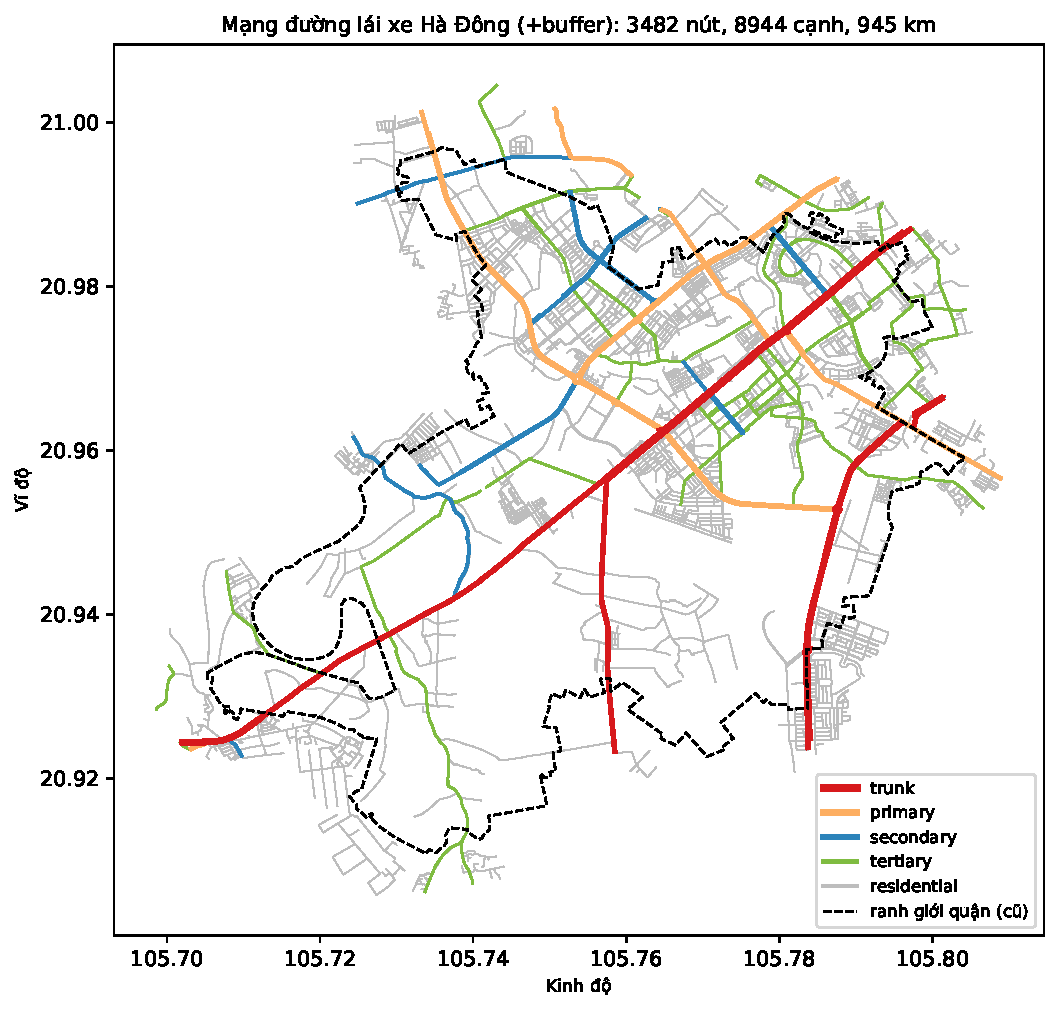
\includegraphics[width=0.72\linewidth]{graph_map.pdf}
\caption{Mạng đường lái xe quận Hà Đông (cộng vùng đệm 500 m) theo nhóm đường; nét đứt là ranh giới quận cũ.}
\label{fig:graph}
\end{figure}

\subsubsection{Mô hình vận tốc 24 khung giờ}\label{sec:method:speed}

Với mỗi cạnh $e$ và mỗi khung giờ $h\in\{0,1,\dots,23\}$, vận tốc nền được xác định bởi một \emph{mức ùn} $c(e,h)\in[0,c_{\max}]$:
\begin{equation}
v(e,h) = \max\Bigl(v_{\text{free}}(e)\bigl(1-c(e,h)\bigr),\; v_{\min}\Bigr),
\label{eq:speed}
\end{equation}
\begin{equation}
\begin{aligned}
c(e,h) = \operatorname{clip}\Bigl(\,&p(h)\cdot s(g_e)\cdot \eta(e,h)\cdot \delta(e,h) + \xi(e,h),\\
&0,\; c_{\max}\Bigr),
\end{aligned}
\label{eq:congestion}
\end{equation}
với $c_{\max}=0{,}85$ và $v_{\min}=5$ km/h. Các thành phần được thiết kế để mỗi thành phần phản ánh một hiện tượng giao
thông có thật:

\textbf{Profile theo giờ $p(h)$} là tổng các hàm Gaussian \emph{tuần hoàn} chu kỳ 24 giờ, bảo đảm tính lặp lại hằng ngày
($p(0)=p(24)$):
\begin{equation}
p(h) = b + \sum_{j} a_j \sum_{k\in\{-1,0,1\}} \exp\!\left(-\frac{(h-\mu_j+24k)^2}{2\sigma_j^2}\right),
\label{eq:profile}
\end{equation}
với các đỉnh sáng ($\mu=8$), trưa ($\mu=12{,}5$), chiều ($\mu=18$), tối ($\mu=21$) và một ``trũng'' ban đêm (biên độ âm,
$\mu=3$); tham số đầy đủ ở Phụ lục.

\textbf{Độ nhạy theo loại đường $s(g)$} phản ánh việc trục chính chịu ùn nặng hơn đường nhánh: trunk 1,0; primary 0,95;
secondary 0,8; tertiary 0,65; residential 0,4.

\textbf{Hệ số trục nóng $\eta(e,h)$} lấy từ tệp \texttt{hotspots.yaml} (Phụ lục): mỗi điểm nóng có hệ số nhân và khung giờ
ảnh hưởng; cạnh được khớp theo tên đường không dấu (loại trừ các ngõ/ngách mang tên trục), theo mã đường (ví dụ QL.6)
hoặc theo bán kính quanh toạ độ nút giao (Cầu Am, Mai Lĩnh, Bến xe Yên Nghĩa).

\textbf{Hệ số hướng $\delta(e,h)$} làm ùn nặng hơn theo hướng vào trung tâm buổi sáng và hướng ra buổi chiều:
\begin{equation}
\delta(e,h) = 1 + \beta\, a_e\,\bigl(w_{\text{sáng}}(h)-w_{\text{chiều}}(h)\bigr), \qquad
a_e = \cos\angle\bigl(\vec{e},\, \vec{c}-\vec{m}_e\bigr),
\label{eq:direction}
\end{equation}
trong đó $\vec{c}$ là toạ độ Ngã Tư Sở (tâm tham chiếu), $\vec{m}_e$ là trung điểm cạnh, $w_{\text{sáng}}, w_{\text{chiều}}$
là các Gaussian tuần hoàn quanh 8h và 18h, $\beta=0{,}3$.

\textbf{Nhiễu không gian $\xi(e,h)$} được tạo bằng cách làm mượt nhiễu Gaussian $k$ lần qua ma trận kề cạnh--cạnh chuẩn
hoá theo hàng $\hat{A}$ (hai cạnh kề nếu chung đầu mút), sau đó chuẩn hoá về độ lệch chuẩn $\sigma_\xi$:
\begin{equation}
\Xi^{(k)} = \hat{A}^{\,k}\,\Xi^{(0)}, \qquad \Xi^{(0)}_{e,h}\sim\mathcal{N}(0,1),
\label{eq:smooth}
\end{equation}
cộng thêm một thành phần nhỏ phụ thuộc ``seed ngày'' để mỗi ngày khác nhau nhưng vẫn cùng quy luật.

\textbf{Nội suy theo phút.} Với $t$ phút, đặt $h=\lfloor (t \bmod 1440)/60\rfloor$ và $\phi=((t\bmod 1440)-60h)/60$; vận tốc
được nội suy tuyến tính (vòng 24 giờ):
\begin{equation}
v_e(t) = (1-\phi)\,v(e,h) + \phi\, v\bigl(e,(h+1)\bmod 24\bigr).
\label{eq:interp}
\end{equation}

\textbf{Bảo đảm FIFO cho vận tốc nền.} Trong một khung giờ, nếu vận tốc tăng tuyến tính từ $v_\ell$ lên $v_u$ thì
$\tau_e(t)=L_e/v_e(t)$ giảm với tốc độ lớn nhất tại đầu mút có vận tốc thấp:
\begin{equation}
\max_t\left(-\frac{d\tau_e}{dt}\right) = \frac{L_e\,(v_u-v_\ell)}{60\,v_\ell^{2}}.
\label{eq:slope}
\end{equation}
Chúng tôi yêu cầu đại lượng này không vượt quá $\kappa=0{,}9<1$ (biên an toàn cho điều kiện \eqref{eq:fifo-deriv}).
Nếu vi phạm, vận tốc đầu mút thấp được nâng lên giá trị nhỏ nhất thoả mãn, tức nghiệm dương của
\begin{equation}
60\kappa\, x^2 + L_e\, x - L_e\, v_u = 0 \;\Longrightarrow\;
x = \frac{-L_e + \sqrt{L_e^2 + 240\kappa L_e v_u}}{120\kappa},
\label{eq:fifo-fix}
\end{equation}
và thủ tục lặp tới khi mọi đoạn thoả mãn (Bổ đề~\ref{bd:fifofix}). Với $V_{\text{base}}$ của Hà Đông, độ dốc lớn nhất
đo được là \FifoSlope{} nên không ô nào cần sửa.

\textbf{Sự cố.} Một sự cố trên cạnh $e$ bắt đầu lúc $t_s$, kéo dài $D$ phút, mức độ $\rho\in[0{,}1;0{,}4]$, nhân vận tốc
với hệ số
\begin{equation}
f(t)=\begin{cases}
1-(1-\rho)\dfrac{t-t_s}{r_{\text{in}}}, & t_s\le t<t_s+r_{\text{in}},\\[2mm]
\rho, & t_s+r_{\text{in}}\le t\le t_s+D,\\[1mm]
\rho+(1-\rho)\dfrac{t-t_s-D}{r_{\text{out}}}, & t_s+D<t<t_s+D+r_{\text{out}},\\[2mm]
1, & \text{ngược lại},
\end{cases}
\label{eq:incident}
\end{equation}
với $r_{\text{in}}=5$ phút (dốc vào) và $r_{\text{out}}=15$ phút (giải toả). Khi sự cố kết thúc, vận tốc tăng nhanh có thể
phá vỡ FIFO. Vì vậy hàm đến của cạnh bị sự cố được tính trên lưới 1 phút rồi \emph{FIFO hoá}:
\begin{equation}
\tilde{a}_e(t) = \min_{t'\ge t} a_e(t'),
\label{eq:fifoize}
\end{equation}
và nội suy tuyến tính giữa các điểm lưới. Về mặt vật lý, \eqref{eq:fifoize} tương ứng với việc xe đến cạnh sớm ``đợi''
ngầm để không về muộn hơn xe đến sau; Mệnh đề~\ref{md:fifoize} chứng minh tính FIFO tuyệt đối của kết quả.

\begin{figure}[H]
\centering
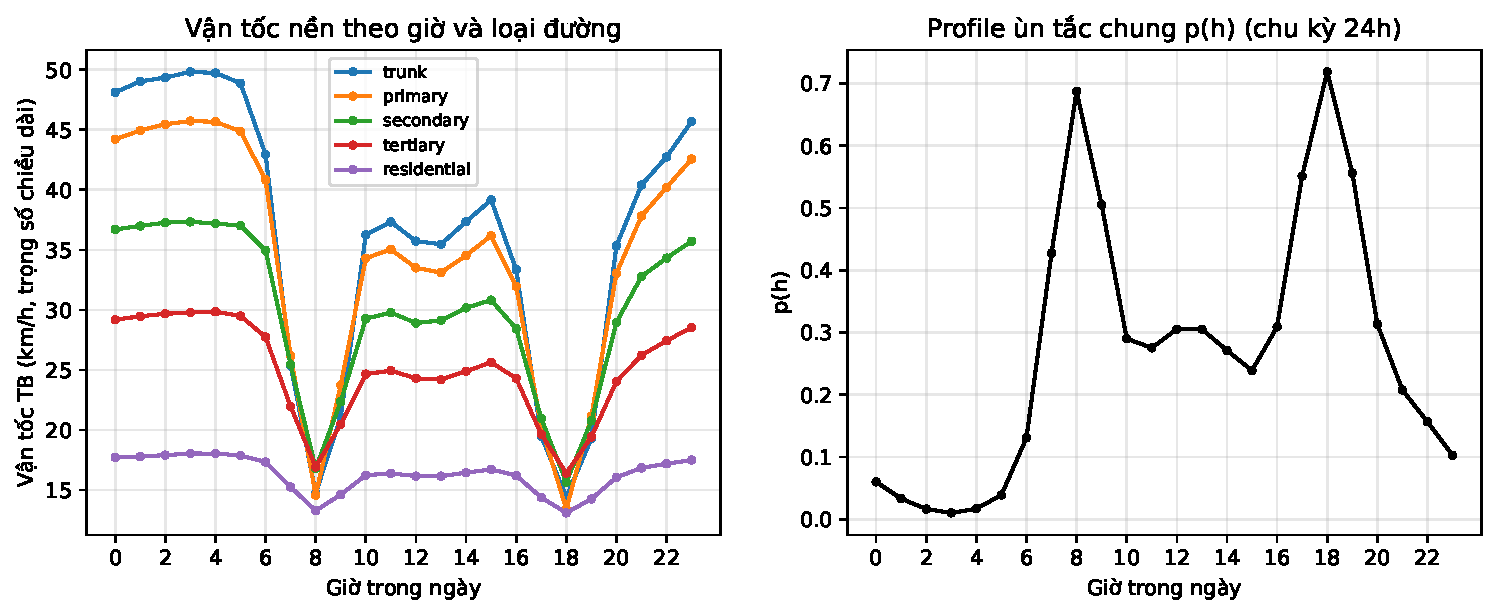
\includegraphics[width=\linewidth]{speed_curves.pdf}
\caption{Vận tốc nền trung bình theo giờ và nhóm đường (trái); profile ùn tắc chung $p(h)$ (phải).}
\label{fig:speedcurves}
\end{figure}

\begin{figure}[H]
\centering
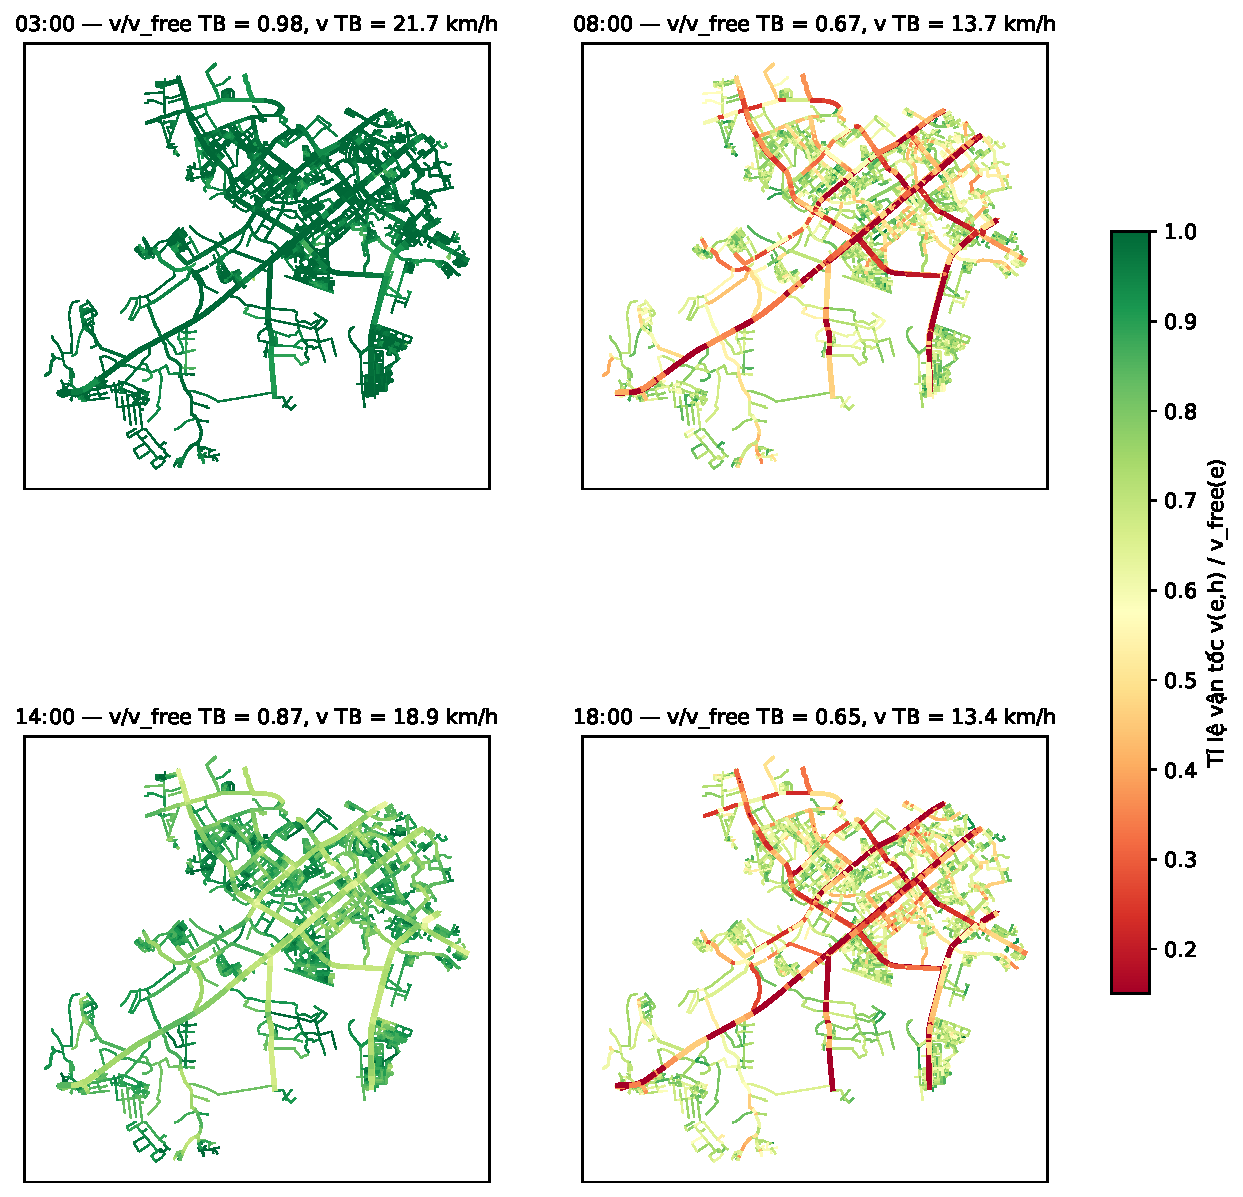
\includegraphics[width=0.82\linewidth]{speed_maps.pdf}
\caption{Tỉ lệ $v/v_{\text{free}}$ trên toàn mạng lúc 3h, 8h, 14h và 18h.}
\label{fig:speedmaps}
\end{figure}

Hình~\ref{fig:speedcurves} và Hình~\ref{fig:speedmaps} cho thấy mô hình tái hiện đúng các hiện tượng mong muốn: vận tốc
trung bình (trọng số theo chiều dài) là \VThree{} km/h lúc 3h, \VEight{} km/h lúc 8h, \VFourteen{} km/h lúc 14h và
\VEighteen{} km/h lúc 18h; vào giờ cao điểm các trục chính chuyển sang màu đỏ.

\subsubsection{Môi trường thực với nhiễu tương quan}\label{sec:method:noise}

Môi trường thực của mỗi truy vấn được sinh từ vận tốc nền và một trường nhiễu nhân:
\begin{equation}
V_{\text{real}} = \mathcal{F}\Bigl(V_{\text{base}}\odot \exp\bigl(\sigma Z\bigr)\Bigr),
\label{eq:vreal}
\end{equation}
trong đó $\mathcal{F}$ là thủ tục sửa FIFO \eqref{eq:fifo-fix}, $\odot$ là tích từng phần tử, $\sigma$ là mức nhiễu của
truy vấn (nhận một trong các giá trị $0{,}05$; $0{,}15$; $0{,}30$). Trường $Z$ có phân phối biên chuẩn tắc $\mathcal{N}(0,1)$ nên hệ số $\varepsilon=e^{\sigma Z}$
tuân theo phân phối LogNormal$(0,\sigma)$; nhưng khác với nhiễu độc lập, $Z$ có \emph{tương quan không gian--thời gian}:
\begin{equation}
Z_{\cdot,h} = \rho\, Z_{\cdot,h-1} + \sqrt{1-\rho^2}\; \hat{A}^{\,k} W_{\cdot,h}, \qquad W_{e,h}\sim\mathcal{N}(0,1),
\label{eq:ar1}
\end{equation}
sau đó chuẩn hoá và trộn với một phần nhiễu độc lập:
\begin{equation}
Z \leftarrow \sqrt{1-\gamma}\; Z + \sqrt{\gamma}\; U, \qquad U_{e,h}\sim\mathcal{N}(0,1),
\label{eq:mix}
\end{equation}
với $\rho=\NoiseRho$, $k=4$, $\gamma=\NoiseIid$. Đo trên trường mẫu, tương quan giữa hai giờ liền kề là \NoiseLagCorr{}
và giữa hai cạnh nối tiếp là \NoiseAdjCorr. Tương quan này là điều kiện để quan sát ở hiện tại và ở lân cận mang thông
tin về tương lai gần và về các cạnh chưa quan sát --- tiền đề của dự báo ngắn hạn ở Mục~\ref{sec:method:gcn}.

\subsubsection{Tìm kiếm phụ thuộc thời gian và heuristic}\label{sec:method:search}

\textbf{TD-Dijkstra} gán cho mỗi nút nhãn $\text{arr}(v)$ là thời điểm đến sớm nhất đã biết. Khi lấy nút $u$ ra khỏi hàng
đợi, mỗi cạnh $e=(u,v)$ được ``nới lỏng'':
\begin{equation}
\text{arr}(v) \leftarrow \min\Bigl(\text{arr}(v),\; \text{arr}(u) + \tau_e\bigl(\text{arr}(u)\bigr)\Bigr).
\label{eq:relax}
\end{equation}
\textbf{TD-A*} ưu tiên các nút theo khoá
\begin{equation}
f(v) = \text{arr}(v) + h(v),
\label{eq:astar-key}
\end{equation}
với $h(v)$ là cận dưới của thời gian còn lại tới đích (Thuật toán~\ref{alg:tdastar}). Chúng tôi cài đặt ba heuristic:

\emph{Heuristic chim bay.} Với $v_{\max}$ là vận tốc lớn nhất toàn cục của mô hình (\VMaxGlobal{} km/h với $V_{\text{base}}$):
\begin{equation}
h_{\text{eu}}(v) = 0{,}995\cdot\frac{\text{dist}(v,d)}{v_{\max}}.
\label{eq:h-eu}
\end{equation}

\emph{Heuristic cận dưới chính xác (LB).} Với mỗi cạnh, thời gian nhỏ nhất qua cạnh trong mọi khung giờ là
\begin{equation}
\tau_{\min}(e) = \frac{L_e}{\max_{h} v(e,h)} \le \tau_e(t)\quad\forall t,
\label{eq:taumin}
\end{equation}
(sự cố chỉ làm chậm nên bất đẳng thức vẫn đúng), và heuristic là khoảng cách ngắn nhất trên đồ thị trọng số $\tau_{\min}$:
\begin{equation}
h_{\text{LB}}(v) = d_{\tau_{\min}}(v,d),
\label{eq:h-lb}
\end{equation}
tính bằng một lần Dijkstra ngược từ đích. Đây là heuristic tĩnh chặt nhất có thể xây từ cận dưới theo từng cạnh.

\emph{Heuristic ALT}~\cite{goldberg2005alt}. Chọn $\mathcal{L}$ gồm 8 điểm mốc theo chiến lược ``điểm xa nhất'' trên đồ
thị $\tau_{\min}$, tiền tính $d(\ell,\cdot)$ và $d(\cdot,\ell)$; heuristic theo bất đẳng thức tam giác:
\begin{equation}
h_{\text{ALT}}(v) = \max_{\ell\in\mathcal{L}} \max\Bigl(d(v,\ell)-d(d,\ell),\; d(\ell,d)-d(\ell,v),\; 0\Bigr).
\label{eq:h-alt}
\end{equation}

\emph{Biên dịch JIT.} Cùng thuật toán TD-A* được viết lại cho Numba~\cite{lam2015numba}, chạy trực tiếp trên mảng CSR và
ma trận vận tốc, cho kết quả và số nút mở rộng trùng khớp với bản Python (đã kiểm chứng bằng kiểm thử đơn vị).
Contraction Hierarchies không được cài đặt: ở quy mô vài nghìn nút, TD-A* biên dịch đã chạy dưới một mili-giây mỗi truy
vấn; CH chỉ thật sự cần thiết khi mở rộng ra toàn thành phố.

\subsubsection{Tái lập kế hoạch}\label{sec:method:replan}

\textbf{Replan.} Tại mỗi giao lộ $u$ ở thời điểm $t$, xe đo độ lệch giữa thời gian thực và dự báo cho mọi cạnh trong bán
kính $r=\ReplanRadius$ m:
\begin{equation}
\delta_e = \tau^{\text{real}}_e(t) - \tau^{\text{base}}_e(t), \qquad e\in\mathcal{N}_r(u),
\label{eq:delta}
\end{equation}
ghi nhớ các độ lệch đã đo, giả định chúng \emph{duy trì} trong tương lai gần và lập lại kế hoạch bằng TD-A* trên mô hình
\begin{equation}
\tau^{\text{obs}}_e(t') = \max\Bigl(\tau^{\text{base}}_e(t') + \delta_e,\; \frac{L_e}{v_{\max}}\Bigr).
\label{eq:tau-obs}
\end{equation}
Cộng một hằng số vào hàm thời gian giữ nguyên tính FIFO, còn cận dưới $L_e/v_{\max}$ giữ heuristic chim bay chấp nhận
được. Xe đi cạnh đầu tiên của kế hoạch mới rồi lặp lại (Thuật toán~\ref{alg:replan}).

\textbf{Replan lười.} Chỉ chạy lại tìm kiếm khi có ít nhất một cạnh quan sát mà độ lệch thay đổi đáng kể so với lúc lập
kế hoạch gần nhất:
\begin{equation}
\exists\, e\in\mathcal{N}_r(u):\quad \bigl|\delta_e^{\text{mới}} - \delta_e^{\text{lúc lập}}\bigr| > \theta\,\tau^{\text{base}}_e(t),
\label{eq:lazy}
\end{equation}
với $\theta=\LazyTheta$; ngược lại xe tiếp tục đi theo kế hoạch cũ.

\textbf{D* Lite với chi phí snapshot.} D* Lite~\cite{koenig2002} tìm kiếm ngược từ đích và duy trì hai giá trị cho mỗi nút:
$g(v)$ và giá trị nhìn trước
\begin{equation}
\text{rhs}(v) = \min_{e=(v,w)} \bigl(c(e) + g(w)\bigr), \qquad \text{rhs}(d)=0,
\label{eq:rhs}
\end{equation}
cùng khoá ưu tiên (với $s$ là vị trí hiện tại và $k_m$ là bù trừ tích luỹ khi xe di chuyển)
\begin{equation}
\text{key}(v) = \Bigl(\min\bigl(g(v),\text{rhs}(v)\bigr) + h(s,v) + k_m,\; \min\bigl(g(v),\text{rhs}(v)\bigr)\Bigr).
\label{eq:dstar-key}
\end{equation}
Vì D* Lite đòi hỏi chi phí tĩnh, ta dùng chi phí \emph{snapshot} $c(e)=\tau^{\text{obs}}_e(t_{\text{snap}})$; giữa hai lần
dựng lại, chỉ các cạnh có quan sát mới được cập nhật và D* Lite chỉ sửa phần lời giải bị ảnh hưởng. Toàn bộ chi phí được
dựng lại sau mỗi \DstarRefresh{} phút di chuyển. Đánh đổi: nhanh hơn TD-A* lặp nhưng bỏ qua biến thiên vận tốc trong
tương lai gần.

\subsubsection{Dự báo ngắn hạn bằng mạng tích chập đồ thị}\label{sec:method:gcn}

Giả định có \SensorFrac\% số cạnh được gắn cảm biến (hoặc có xe thăm dò), gồm mọi trục trunk/primary và một phần ngẫu
nhiên các cạnh khác (tổng cộng \NSensors{} cạnh). Tại thời điểm $t$, ta quan sát log-tỉ số vận tốc
\begin{equation}
r_e(t) = \log\frac{v^{\text{real}}_e(t)}{v^{\text{base}}_e(t)} = \log\frac{\tau^{\text{base}}_e(t)}{\tau^{\text{real}}_e(t)}
\label{eq:logratio}
\end{equation}
trên các cạnh có cảm biến và các cạnh trong bán kính quan sát. Đặc trưng đầu vào của cạnh $e$ là
$x_e=[\,r_e\mathbf{1}_e,\ \mathbf{1}_e,\ \text{onehot}(g_e),\ \sin\omega t,\ \cos\omega t,\ c(e,h)\,]$ với $\mathbf{1}_e$ là cờ
``đã quan sát''. Mạng tích chập đồ thị~\cite{kipf2017gcn} trên đồ thị cạnh--cạnh gồm
\begin{equation}
H^{(0)} = \operatorname{ReLU}\bigl(XW_0\bigr), \qquad
H^{(\ell+1)} = \operatorname{ReLU}\Bigl(\hat{A}H^{(\ell)}W_1^{(\ell)} + H^{(\ell)}W_2^{(\ell)}\Bigr),
\label{eq:gcn}
\end{equation}
với 3 lớp ẩn kích thước 32, đầu ra $\hat{y}_e\in\mathbb{R}^2$ là log-tỉ số dự đoán tại hai mốc giờ $h$ và $h+1$. Hàm mất mát
là sai số bình phương trung bình trên mọi cạnh:
\begin{equation}
\mathcal{L}_{\text{GCN}} = \frac{1}{2m}\sum_{e\in E}\bigl\|\hat{y}_e - y_e\bigr\|_2^2,
\label{eq:gcn-loss}
\end{equation}
huấn luyện bằng Adam trên các ``ngày'' mô phỏng có seed độc lập với tập kiểm tra. Với các mốc giờ xa hơn, dự báo tắt dần
theo hệ số tự tương quan:
\begin{equation}
\hat{r}_e(h+k) = \rho^{\,k-1}\,\hat{y}_{e,2}, \qquad k\ge 2,
\label{eq:decay}
\end{equation}
rồi ma trận vận tốc dự báo $V_{\text{base}}\odot e^{\hat r}$ được đưa vào TD-A*. Hai cách dùng: \emph{plan-once + GCN}
(dự báo một lần lúc xuất phát) và \emph{replan + GCN} (cập nhật GCN mỗi \GcnRecompute{} phút; các cạnh vừa quan sát vẫn
dùng độ lệch đo trực tiếp \eqref{eq:delta}). Đối chứng \emph{plan-once + cảm biến} chỉ dùng độ lệch trên chính các cạnh
có cảm biến mà không lan truyền sang cạnh khác.

\subsubsection{Định tuyến theo rủi ro (P90)}\label{sec:method:risk}

Một ``ngân hàng kịch bản'' gồm $M=\RiskM$ ma trận vận tốc được sinh từ cùng mô hình nhiễu \eqref{eq:vreal} với seed độc
lập với tập kiểm tra. Tập ứng viên $\mathcal{C}$ gồm $\RiskK$ tuyến của thuật toán Yen theo thời gian qua cạnh tại giờ xuất
phát, cộng tuyến TD-A* theo dự báo. Phân vị 90\% của mỗi ứng viên được ước lượng bằng phân vị thực nghiệm trên các kịch bản
và chọn
\begin{equation}
\hat{P} = \arg\min_{P\in\mathcal{C}}\; \widehat{Q}_{0.9}\Bigl\{T^{(j)}(P,t_0)\Bigr\}_{j=1}^{M},
\label{eq:risk-est}
\end{equation}
trong đó $T^{(j)}(P,t_0)$ là thời gian đi tuyến $P$ trong kịch bản $j$, được tính vector hoá đồng thời cho cả $M$ kịch bản.

\subsubsection{Học tăng cường}\label{sec:method:rl}

\textbf{Môi trường.} Môi trường chuẩn Gymnasium: tác tử đứng tại một nút và chọn một trong $K=\MaxOutDeg$ khe cạnh ra
(khe trống bị che bằng mặt nạ). Mỗi tập lấy một cặp điểm đi--đến của tập huấn luyện, với giờ xuất phát, seed nhiễu và sự
cố được sinh \emph{mới} để tác tử không học thuộc. Quan sát \emph{cục bộ} gồm vị trí tương đối tới đích (chuẩn hoá 8 km),
khoảng cách chim bay, $\sin/\cos$ của giờ, tỉ lệ số bước đã dùng; và với mỗi khe cạnh ra: cờ hợp lệ, vận tốc quan sát
hiện tại (nhiễu 5\%) chia 60 km/h, chiều dài chia 500 m, cosin góc giữa cạnh và hướng tới đích, cờ ``nút cuối đã thăm''.

\textbf{Phần thưởng.} Khi đi cạnh $e$ mất $\tau$ phút từ nút $u$ tới nút $u'$:
\begin{equation}
\begin{aligned}
r = -\tau + \lambda\,F(u,u') &+ R_{\text{goal}}\,\mathbf{1}[u'=d] \\
&- R_{\text{rev}}\,\mathbf{1}[u'\ \text{đã thăm}] - R_{\text{out}}\,\mathbf{1}[\text{quá số bước}],
\end{aligned}
\label{eq:reward}
\end{equation}
với $R_{\text{goal}}=10$, $R_{\text{rev}}=1$, $R_{\text{out}}=10$, giới hạn số bước bằng $3\times$ số cạnh của tuyến tham chiếu
cộng 20. Thành phần định hình $F$ có hai dạng: theo khoảng cách chim bay (quy ra phút ở 30 km/h), hoặc \emph{theo thế
năng cost-to-go}~\cite{ng1999}:
\begin{equation}
F(u,u') = \Phi(u') - \Phi(u), \qquad \Phi(u) = -\,\text{ctg}_{\text{tự do}}(u),
\label{eq:shaping}
\end{equation}
trong đó $\text{ctg}_{\text{tự do}}(u)$ là thời gian tự do ngắn nhất từ $u$ tới đích. Thông tin toàn cục này chỉ nằm trong
\emph{phần thưởng} lúc huấn luyện; chính sách không quan sát được nó (Mệnh đề~\ref{md:shaping}).

\textbf{Thuật toán học.} MaskablePPO (sb3-contrib) tối ưu hàm mục tiêu cắt xén của PPO~\cite{schulman2017}:
\begin{equation}
\begin{gathered}
\mathcal{L}^{\text{CLIP}}(\theta) = \mathbb{E}_t\Bigl[\min\bigl(\varrho_t(\theta)\hat{A}_t,\;
\operatorname{clip}(\varrho_t(\theta),1-\epsilon,1+\epsilon)\hat{A}_t\bigr)\Bigr],\\[1mm]
\varrho_t(\theta)=\frac{\pi_\theta(a_t\mid o_t)}{\pi_{\theta_{\text{old}}}(a_t\mid o_t)},
\end{gathered}
\label{eq:ppo}
\end{equation}
với $\hat{A}_t$ là ước lượng lợi thế GAE, $\epsilon=0{,}2$, hệ số chiết khấu $0{,}995$; xác suất của hành động bị che bằng
mặt nạ được đặt bằng 0 trước khi chuẩn hoá~\cite{huang2022}. Huấn luyện theo chương trình ba mức~\cite{bengio2009}: mức 1
(cặp điểm gần dưới 2,5 km, không nhiễu) tới 20\% số bước; mức 2 (mọi cặp, có nhiễu) tới 50\%; mức 3 (thêm sự cố).

\textbf{Các biến thể} (Bảng~\ref{tab:rl-variants}):
\begin{itemize}
    \item \emph{RL cục bộ} --- đúng đặc tả ban đầu: quan sát cục bộ, định hình theo khoảng cách chim bay.
    \item \emph{RL + ctg (quan sát)} --- thí nghiệm đối chứng: thêm cost-to-go tự do (thông tin toàn cục tĩnh) vào quan sát.
    \item \emph{RL + định hình ctg} --- quan sát cục bộ, định hình thưởng theo \eqref{eq:shaping}.
    \item \emph{RL cây-GNN} --- quan sát cây lân cận \TreeDepth{} bước ($K+K^2+K^3$ khe, mỗi khe thêm cờ ngõ cụt, cờ quay đầu,
    tiến độ tới đích). Bộ trích đặc trưng truyền thông điệp từ lá lên gốc với trọng số dùng chung giữa các khe cùng tầng:
    \begin{equation}
    \begin{gathered}
    m_D(j) = \phi_D\bigl(x_D(j)\bigr),\\[1mm]
    m_d(j) = \phi_d\Bigl(\bigl[\,x_d(j)\ \|\ \max_{c\in\text{con}(j)} m_{d+1}(c)\,\bigr]\Bigr),\quad d=D-1,\dots,1,
    \end{gathered}
    \label{eq:tree-gnn}
    \end{equation}
    và vector đặc trưng đưa vào chính sách là $[\psi(x_{\text{glob}}),\, m_1(1),\dots,m_1(K)]$ --- mỗi nhánh tầng 1 ứng với
    một hành động, nên chính sách ``nhìn'' được phía sau mỗi cạnh ra tới $D$ bước.
    \item \emph{RL LSTM} --- RecurrentPPO với LSTM~\cite{hochreiter1997lstm} có 128 đơn vị ẩn. Vì sb3-contrib không hỗ trợ mặt nạ
    cho RecurrentPPO, hành động $a$ được ánh xạ thành $a \bmod \deg^+(u)$.
    \item \emph{RL cây-GNN + BC} --- trước khi chạy PPO, chính sách được học bắt chước từ oracle. Dữ liệu thu theo kiểu DAgger
    nhẹ~\cite{ross2011dagger}: thực thi hành động ngẫu nhiên với xác suất 20\%, còn nhãn luôn là cạnh tiếp theo của tuyến
    oracle tính lại từ trạng thái hiện tại. Hàm mất mát là log-likelihood âm:
    \begin{equation}
    \mathcal{L}_{\text{BC}}(\theta) = -\frac{1}{|\mathcal{D}|}\sum_{(o,a^\ast,\mu)\in\mathcal{D}} \log \pi_\theta\bigl(a^\ast\mid o,\mu\bigr),
    \label{eq:bc}
    \end{equation}
    với $\mu$ là mặt nạ hành động; sau đó tinh chỉnh bằng PPO với tốc độ học nhỏ hơn ($10^{-4}$).
    \item \emph{RL lai (RL + tìm kiếm)} --- hành động là hệ số $\beta\in\{0;\,0{,}5;\,1;\,2;\,4\}$ thể hiện mức tin vào quan sát;
    TD-A* lập kế hoạch trên
    \begin{equation}
    \tau^{(\beta)}_e(t) = \max\Bigl(\tau^{\text{base}}_e(t) + \beta\,\delta_e,\; \frac{L_e}{v_{\max}}\Bigr)
    \label{eq:hybrid}
    \end{equation}
    và xe đi cạnh đầu tiên. $\beta=1$ chính là replan, $\beta=0$ là chỉ dùng dự báo, $\beta>1$ là né vùng chậm mạnh tay hơn;
    quan sát gồm 12 đặc trưng tóm tắt (khoảng cách, giờ, thống kê độ lệch quan sát, độ trễ so với kế hoạch). Vì TD-A* luôn
    tìm được đường trên đồ thị liên thông mạnh, tác tử \emph{luôn} tới đích.
\end{itemize}

\begin{table}[H]
\centering\small
\renewcommand{\arraystretch}{1.2}
\caption{Các biến thể học tăng cường (mỗi biến thể huấn luyện với 3 seed).}
\label{tab:rl-variants}
\begin{tabularx}{\linewidth}{>{\raggedright\arraybackslash}p{3.2cm}>{\raggedright\arraybackslash}p{3.3cm}>{\raggedright\arraybackslash}p{2.6cm}X}
\toprule
\textbf{Biến thể} & \textbf{Quan sát} & \textbf{Thuật toán} & \textbf{Điểm khác biệt} \\
\midrule
RL cục bộ & cục bộ ($K$ cạnh ra) & MaskablePPO & đặc tả gốc, định hình chim bay \\
RL + ctg (quan sát) & cục bộ + cost-to-go & MaskablePPO & đối chứng có thông tin toàn cục \\
RL + định hình ctg & cục bộ & MaskablePPO & định hình thưởng theo thế năng \\
RL cây-GNN & cây \TreeDepth{} bước & MaskablePPO + GNN & quan sát rộng hơn \\
RL LSTM & cục bộ & RecurrentPPO & bộ nhớ (không có mặt nạ) \\
RL cây-GNN + BC & cây \TreeDepth{} bước & MaskablePPO + GNN & học bắt chước oracle trước \\
RL lai & 12 đặc trưng tóm tắt & MaskablePPO & RL chọn $\beta$, TD-A* tìm đường \\
\bottomrule
\end{tabularx}
\end{table}

\subsubsection{Chọn giờ xuất phát}\label{sec:method:departure}

Tác tử quyết định ``đi ngay'' hay ``chờ thêm \WaitStep{} phút'' (tối đa \MaxWaits{} lần). Trạng thái gồm khung 30 phút
trong ngày, số lần đã chờ, nhóm khoảng cách và nhóm mức ùn \emph{dự báo} của chính cặp điểm đi--đến
($T^{\text{dự báo}}(t)/T^{\text{tự do}}$) --- thông tin có sẵn tại thời điểm quyết định. Q-learning dạng bảng~\cite{watkins1992}
cập nhật
\begin{equation}
Q(s,a) \leftarrow Q(s,a) + \alpha\Bigl[r + \gamma\max_{a'}Q(s',a') - Q(s,a)\Bigr],
\label{eq:qlearning}
\end{equation}
với phần thưởng $r=-w\Delta$ khi chờ và $r=-T^{\text{oracle}}(t)$ khi đi. Vì $Q$ khởi tạo bằng 0 trong khi mọi phần thưởng
đều âm, các ô ít được ghé sẽ trông ``lạc quan''; khi ra quyết định chúng tôi chỉ tin $Q$ ở những ô đã được cập nhật ít
nhất \DepMinVisits{} lần, ngược lại mặc định đi ngay.

\subsubsection{Mô phỏng nhiều xe}\label{sec:method:multi}

Mỗi tác tử đại diện cho 20 xe, xuất phát ngẫu nhiên trong khung 7:30--8:00. Tải dẫn đường trên mỗi cạnh trong từng khung
15 phút làm chậm cạnh theo hàm BPR \eqref{eq:bpr} với $\alpha=0{,}5$, $\beta=2$ và năng lực theo nhóm đường. Hai chiến lược:
\emph{dẫn đường giống nhau} (mọi xe chạy TD-A* trên dự báo, không biết xe khác) và \emph{phối hợp tuần tự} (lập kế hoạch
lần lượt theo giờ xuất phát, mỗi xe thấy tải của các xe đã lập trước). Thời gian đi thực tế được tính bằng lặp điểm bất
động giữa tải và lịch trình trên các tuyến cố định.

\subsubsection{Ứng dụng minh hoạ và đóng gói}\label{sec:method:app}

Ứng dụng Streamlit (Hình~\ref{fig:app}) cho phép nhấp bản đồ để đặt điểm đi/đến hoặc vị trí sự cố, chọn giờ và phương
pháp (Dijkstra, TD-A*, replan, D* Lite, P90 và các biến thể RL đã huấn luyện), hiển thị bảng thời gian dự kiến/thực tế
cùng các phân vị P10/P50/P90 trên ngân hàng kịch bản, $k$ tuyến thay thế, lớp màu vận tốc (gộp theo 5 lớp màu, có chú
thích), đường cong thời gian đi theo 24 giờ xuất phát kèm dải P10--P90, và một thẻ vẽ toàn bộ \NEdges{} cạnh bằng WebGL.
Toàn bộ dự án được đóng gói bằng Docker (PyTorch bản CPU) và đã được kiểm tra chạy trong container.

\begin{figure}[H]
\centering
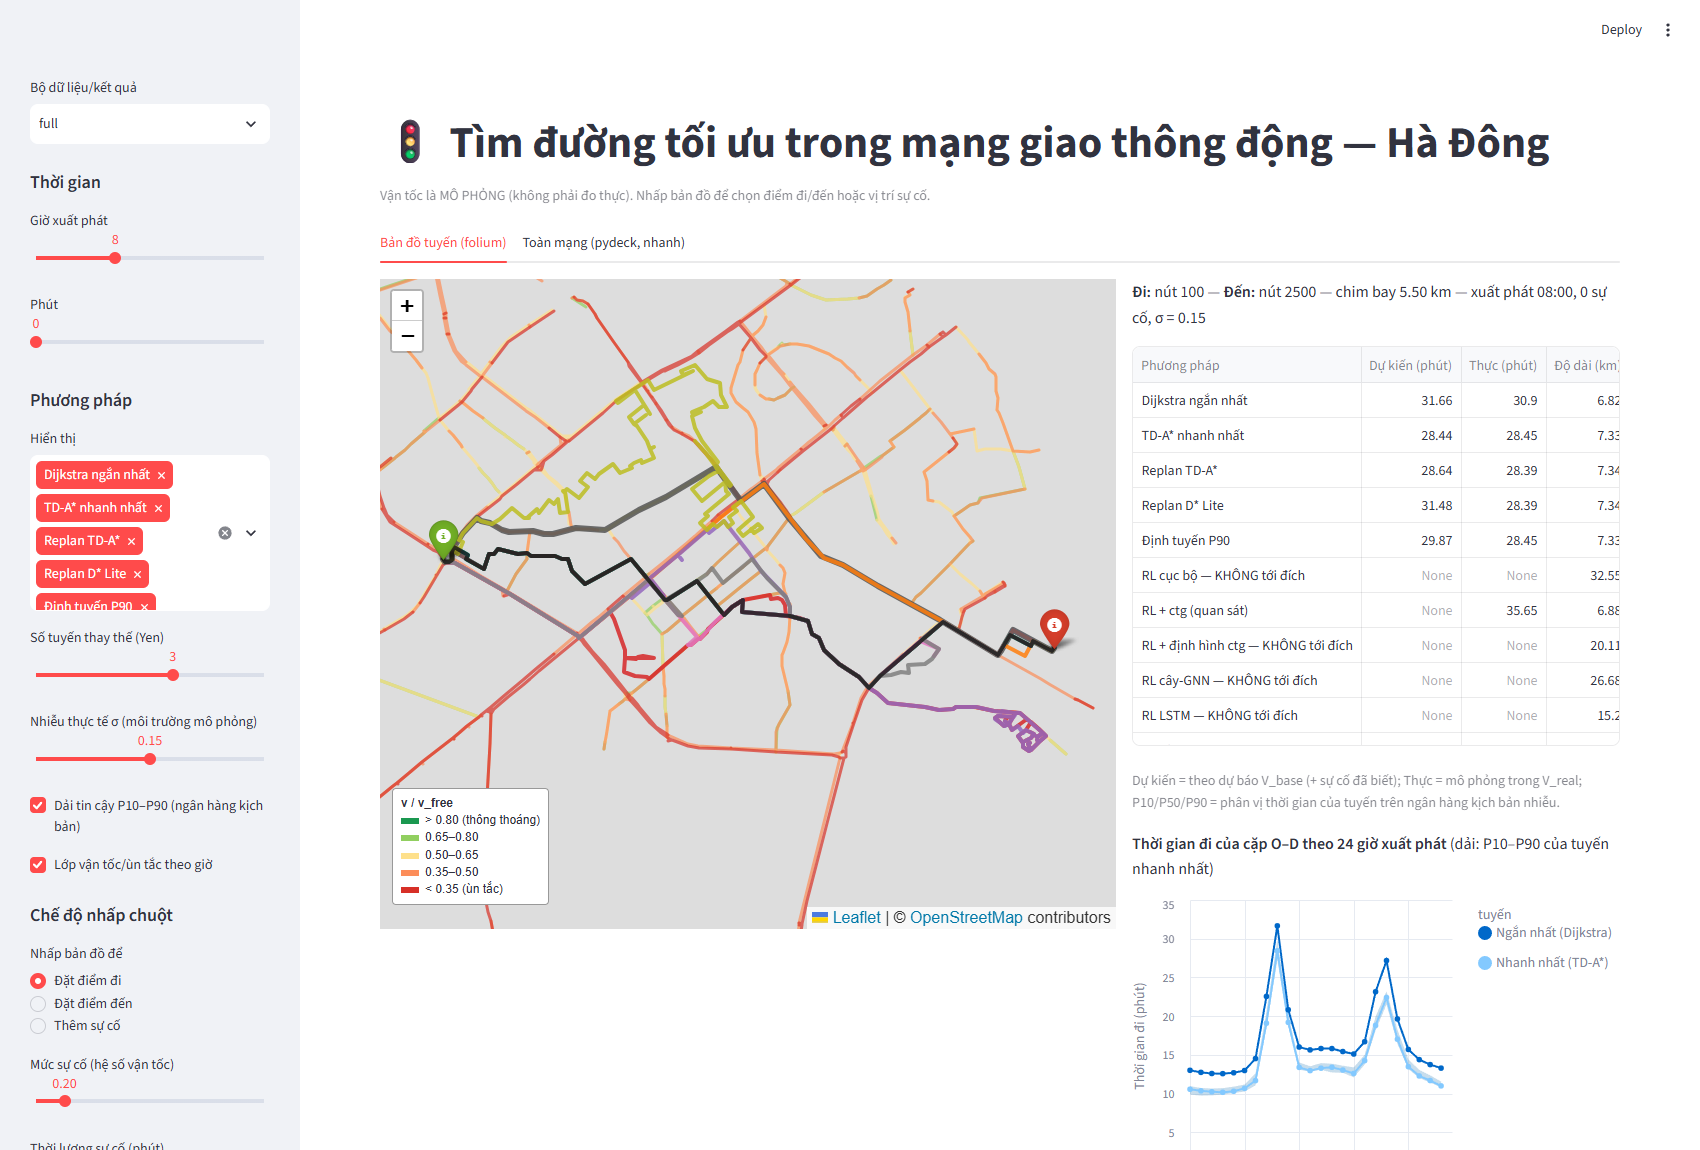
\includegraphics[width=\linewidth]{app_screenshot.png}
\caption{Giao diện ứng dụng minh hoạ (chụp tự động; nền bản đồ không tải trong trình duyệt chạy ẩn).}
\label{fig:app}
\end{figure}

\subsection{Phân tích độ phức tạp / tính đúng đắn}\label{sec:method:correct}

\begin{dl}\label{dl:tdd}
Nếu mọi hàm đến $a_e$ không giảm (FIFO) và $\tau_e(t)>0$, TD-Dijkstra trả về thời điểm đến sớm nhất tại $d$ khi xuất phát từ
$s$ lúc $t_0$.
\end{dl}
\begin{cm}
Gọi $T^\ast(v)$ là thời điểm đến sớm nhất tại $v$. Trước hết, nhờ FIFO, mỗi tiền tố của một đường tối ưu có thể chọn là
tối ưu: nếu đường tối ưu tới $v$ đi qua $x$ ở thời điểm $t_x>T^\ast(x)$, thay tiền tố tới $x$ bằng đường đến $x$ lúc $T^\ast(x)$
rồi đi tiếp cùng dãy cạnh; do mọi $a_e$ không giảm, thời điểm đến $v$ không muộn hơn. Bây giờ quy nạp theo thứ tự lấy nút
ra khỏi hàng đợi: giả sử mọi nút đã đóng có nhãn bằng $T^\ast$. Khi lấy $u$ ra, xét đường tối ưu tới $u$ và nút $y$ đầu tiên
trên đó chưa đóng, với nút liền trước $x$ đã đóng. Khi đóng $x$, cạnh $(x,y)$ đã được nới lỏng nên
$\text{arr}(y)\le a_{xy}(T^\ast(x))=T^\ast(y)\le T^\ast(u)$, bất đẳng thức cuối do $\tau>0$. Vì $u$ được chọn trước $y$ nên
$\text{arr}(u)\le\text{arr}(y)\le T^\ast(u)$; mặt khác $\text{arr}(u)\ge T^\ast(u)$ theo định nghĩa. Vậy $\text{arr}(u)=T^\ast(u)$.
\end{cm}

\begin{md}\label{md:heur}
Các heuristic $h_{\text{eu}}$ \eqref{eq:h-eu}, $h_{\text{LB}}$ \eqref{eq:h-lb} và $h_{\text{ALT}}$ \eqref{eq:h-alt} đều chấp nhận được
và nhất quán: $h(u)\le\tau_e(t)+h(v)$ với mọi $e=(u,v)$ và mọi $t$. Do đó TD-A* trả về lời giải tối ưu và mỗi nút được mở
rộng tối đa một lần.
\end{md}
\begin{cm}
Từ \eqref{eq:taumin} và việc chiều dài cạnh được ép không nhỏ hơn khoảng cách hai đầu:
$\tau_e(t)\ge\tau_{\min}(e)\ge L_e/v_{\max}\ge \text{dist}(u,v)/v_{\max}$. Với $h_{\text{eu}}$: bất đẳng thức tam giác cho
$\text{dist}(u,d)\le\text{dist}(u,v)+\text{dist}(v,d)$. Với $h_{\text{LB}}$: theo định nghĩa khoảng cách ngắn nhất,
$d_{\tau_{\min}}(u,d)\le\tau_{\min}(e)+d_{\tau_{\min}}(v,d)$. Với $h_{\text{ALT}}$: mỗi số hạng trong \eqref{eq:h-alt} là cận dưới
nhất quán theo bất đẳng thức tam giác trên đồ thị $\tau_{\min}$~\cite{goldberg2005alt}, và cực đại của các heuristic nhất
quán vẫn nhất quán. Hệ số an toàn nhỏ hơn 1 chỉ làm $h$ nhỏ đi. Cuối cùng, với $h$ nhất quán, hàng đợi theo khoá
\eqref{eq:astar-key} tương đương TD-Dijkstra trên trọng số rút gọn không âm, nên Định lý~\ref{dl:tdd} áp dụng được.
\end{cm}

\begin{bd}\label{bd:fifofix}
Thủ tục \eqref{eq:fifo-fix} chỉ làm tăng vận tốc, dừng sau hữu hạn bước, và kết quả thoả $-d\tau_e/dt\le\kappa<1$ trên mọi
đoạn, do đó thoả FIFO.
\end{bd}
\begin{cm}
Với $v_u$ cố định, vế phải của \eqref{eq:slope} giảm ngặt khi $v_\ell$ tăng, nên giá trị $x$ trong \eqref{eq:fifo-fix} là
vận tốc nhỏ nhất làm độ dốc bằng $\kappa$; thay $v_\ell$ bằng $\max(v_\ell,x)$ chỉ làm vận tốc tăng. Mỗi lần sửa có thể làm
đoạn kề phía trước vi phạm, nhưng dãy vận tốc ở mỗi ô là không giảm và bị chặn trên bởi vận tốc lớn nhất của các ô kề,
nên thủ tục hội tụ. Khi không còn vi phạm, $-\tau'\le\kappa<1$, tức \eqref{eq:fifo-deriv} thoả.
\end{cm}

\begin{md}\label{md:fifoize}
Hàm $\tilde a$ trong \eqref{eq:fifoize} không giảm, $\tilde a\le a$, và $\tilde a(t)=a(t)$ tại mọi $t$ mà $a$ đã không giảm trên $[t,\infty)$.
\end{md}
\begin{cm}
Với $t_1\le t_2$, tập $\{t'\ge t_2\}\subseteq\{t'\ge t_1\}$ nên $\tilde a(t_1)\le\tilde a(t_2)$. Chọn $t'=t$ cho
$\tilde a(t)\le a(t)$. Nếu $a$ không giảm trên $[t,\infty)$ thì cực tiểu đạt tại $t'=t$. Nội suy tuyến tính giữa các điểm lưới
của một dãy không giảm vẫn là hàm không giảm.
\end{cm}

\begin{md}\label{md:shaping}
Định hình \eqref{eq:shaping} là định hình theo thế năng nên (với hệ số chiết khấu xấp xỉ 1) không làm thay đổi tập chính
sách tối ưu~\cite{ng1999}; tổng định hình trên mọi quỹ đạo từ $s$ tới đích bằng $\lambda\,\text{ctg}_{\text{tự do}}(s)$, không
phụ thuộc đường đi.
\end{md}
\begin{cm}
Tổng $\sum_k \bigl(\Phi(u_{k+1})-\Phi(u_k)\bigr)$ là tổng lồng nhau, bằng $\Phi(d)-\Phi(s)=\text{ctg}(s)$ vì $\text{ctg}(d)=0$.
Hằng số này chỉ phụ thuộc trạng thái đầu nên không làm thay đổi thứ tự giữa các chính sách. Tính chất này được kiểm
chứng bằng kiểm thử đơn vị.
\end{cm}

\textbf{Độ phức tạp.} Với hàng đợi nhị phân và việc tính $\tau_e(t)$ mất $O(1)$, độ phức tạp của các thành phần chính được
tổng hợp trong Bảng~\ref{tab:complexity} (ở đây $m/n\approx\MeanOutDeg$; $L$ là số điểm mốc; $S$ là số giao lộ trên tuyến;
$\ell$, $H$ là số lớp và kích thước lớp ẩn của GCN; $M$, $k$ là số kịch bản và số ứng viên; $N$ là số xe; $I$ là số vòng
lặp điểm bất động).

\begin{table}[H]
\centering\small
\renewcommand{\arraystretch}{1.25}
\caption{Độ phức tạp thời gian và bộ nhớ của các thành phần.}
\label{tab:complexity}
\begin{tabularx}{\linewidth}{>{\raggedright\arraybackslash}p{4.2cm}>{\raggedright\arraybackslash}X>{\raggedright\arraybackslash}p{3.2cm}}
\toprule
\textbf{Thành phần} & \textbf{Thời gian} & \textbf{Bộ nhớ} \\
\midrule
TD-Dijkstra / TD-A* & $O((n+m)\log n)$ mỗi truy vấn & $O(n+m)$ \\
Heuristic LB & $+\,O((n+m)\log n)$ mỗi đích & $O(n)$ \\
Heuristic ALT & tiền xử lý $O(L(n+m)\log n)$; mỗi $h(v)$ là $O(L)$ & $O(Ln)$ \\
Replan / replan lười & $O(S(n+m)\log n)$ / $O(S'(n+m)\log n)$, $S'\le S$ & $O(n+m)$ \\
D* Lite & dựng lại $O((n+m)\log n)$; cập nhật tăng dần chỉ các nút đổi khoá & $O(n+m)$ \\
Suy luận GCN & $O(\ell\cdot\text{nnz}(\hat{A})\cdot H)$ & $O(mH)$ \\
Định tuyến P90 & $O(k\cdot\text{Yen} + M\,k\,|P|)$ & $O(M\,m\cdot 24)$ \\
Mô phỏng nhiều xe & $O(N\cdot\text{TD-A*} + I\,N\,|P|)$ & $O(m\cdot \#\text{khung})$ \\
Chính sách RL & $O(|P|)$ lượt suy luận mạng; biến thể lai thêm một TD-A* mỗi bước & số tham số mạng \\
\bottomrule
\end{tabularx}
\end{table}

\subsection{Lược đồ hoặc sơ đồ minh hoạ}\label{sec:method:diagram}

Hình~\ref{fig:pipeline} là sơ đồ khối luồng dữ liệu của toàn hệ thống. Thuật toán~\ref{alg:tdastar} và
Thuật toán~\ref{alg:replan} là mã giả của hai thành phần tìm kiếm cốt lõi; Thuật toán~\ref{alg:bc} mô tả quy trình huấn
luyện biến thể RL cây-GNN + BC.

\begin{figure}[H]
\centering
\begin{adjustbox}{max width=\linewidth}
\begin{tikzpicture}[font=\footnotesize,
  box/.style={draw, rounded corners, align=center, minimum height=11mm, text width=3.0cm, fill=#1!12},
  box/.default=blue, arr/.style={-{Stealth[length=2mm]}, thick}]
\node[box=gray] (osm)   at (0,0)    {OpenStreetMap\\(OSMnx, Overpass)};
\node[box]      (graph) at (3.8,0)  {Đồ thị CSR\\làm sạch, chuẩn hoá};
\node[box]      (speed) at (7.6,0)  {Vận tốc 24 khung giờ\\$V_{\text{base}}$ + FIFO};
\node[box]      (scen)  at (11.4,0) {Kịch bản cố định\\train / val / test};
\node[box=orange] (real) at (7.6,-2) {Môi trường thực\\nhiễu tương quan + sự cố};
\node[box=green] (search) at (3.8,-4)  {TD-A* (chim bay/LB/\\ALT/Numba), replan,\\lười, D* Lite};
\node[box=green] (fc)     at (7.6,-4)  {Dự báo GCN\\(cảm biến), P90};
\node[box=red]   (rl)     at (11.4,-4) {RL: cục bộ, cây-GNN,\\LSTM, BC, lai $\beta$};
\node[box=red]    (dep)  at (0,-6)    {Chọn giờ (Q-learning)\\nhiều xe (BPR)};
\node[box=violet] (eval) at (7.6,-6)  {Đánh giá: regret, CI,\\Wilcoxon, đơn luồng};
\node[box=violet] (out)  at (7.6,-8)  {Hình, bảng LaTeX, macro,\\báo cáo, ứng dụng};
\draw[arr] (osm) -- (graph);
\draw[arr] (graph) -- (speed);
\draw[arr] (speed) -- (scen);
\draw[arr] (speed) -- (real);
\draw[arr] (real) -- (search);
\draw[arr] (real) -- (fc);
\draw[arr] (real) -- (rl);
\draw[arr] (search) -- (dep);
\draw[arr] (search) -- (eval);
\draw[arr] (fc) -- (eval);
\draw[arr] (rl) -- (eval);
\draw[arr] (dep) -- (eval);
\draw[arr] (scen.east) -- ++(0.35,0) |- (eval.east);
\draw[arr] (eval) -- (out);
\end{tikzpicture}
\end{adjustbox}
\caption{Sơ đồ khối của hệ thống: luồng dữ liệu từ OpenStreetMap tới đánh giá và báo cáo.}
\label{fig:pipeline}
\end{figure}

\begin{algorithm}[H]
\caption{TD-A* (nhãn là thời điểm đến)}\label{alg:tdastar}
\begin{algorithmic}[1]
\Require Đồ thị $G$, nguồn $s$, đích $d$, giờ $t_0$, hàm $\tau_e(t)$, heuristic nhất quán $h$
\Ensure Tuyến đến sớm nhất và thời điểm đến
\State $\text{arr}[s]\gets t_0$; $Q\gets\{(t_0+h(s),s)\}$; $C\gets\emptyset$
\While{$Q\neq\emptyset$}
  \State $(\cdot,u)\gets$ \Call{PopMin}{$Q$}; \textbf{if} $u\in C$ \textbf{then continue}
  \State $C\gets C\cup\{u\}$; \textbf{if} $u=d$ \textbf{then return} truy vết$(\text{pred},d)$, $\text{arr}[d]$
  \For{$e=(u,v)\in\text{out}(u)$ với $v\notin C$}
    \State $t'\gets\text{arr}[u]+\tau_e(\text{arr}[u])$ \Comment{nới lỏng \eqref{eq:relax}}
    \If{$t'<\text{arr}[v]$}
      \State $\text{arr}[v]\gets t'$; $\text{pred}[v]\gets e$; \Call{Push}{$Q,(t'+h(v),v)$}
    \EndIf
  \EndFor
\EndWhile
\end{algorithmic}
\end{algorithm}

\begin{algorithm}[H]
\caption{Replan (tuỳ chọn lười) với quan sát cục bộ và dự báo GCN}\label{alg:replan}
\begin{algorithmic}[1]
\Require $s,d,t_0$; dự báo $\tau^{\text{base}}$; môi trường thực $\tau^{\text{real}}$; bán kính $r$; ngưỡng $\theta$ (chế độ lười)
\State $u\gets s$; $t\gets t_0$; $\Delta\gets\{\}$; $P\gets[\,]$
\While{$u\neq d$}
  \State cần $\gets (P=[\,])$ \Comment{chế độ đầy đủ: luôn đặt cần $\gets$ true}
  \For{mỗi cạnh $e$ có nút đầu cách $u$ không quá $r$}
    \State $\delta\gets\tau^{\text{real}}_e(t)-\tau^{\text{base}}_e(t)$ \Comment{\eqref{eq:delta}}
    \If{$|\delta-\Delta_{\text{lúc lập}}[e]|>\theta\,\tau^{\text{base}}_e(t)$} cần $\gets$ true \EndIf \Comment{\eqref{eq:lazy}}
    \State $\Delta[e]\gets\delta$
  \EndFor
  \If{cần}
    \State $\tau^{\text{base}}\gets$ GCN(cảm biến, quan sát) nếu dùng dự báo GCN \Comment{\eqref{eq:gcn}}
    \State $P\gets$ TD-A*$(u,d,t)$ trên $\tau^{\text{obs}}$ \Comment{\eqref{eq:tau-obs}}
  \EndIf
  \State $e\gets$ \Call{PopFront}{$P$}; $t\gets t+\tau^{\text{real}}_e(t)$; $u\gets\text{head}(e)$
\EndWhile
\State \Return $t-t_0$
\end{algorithmic}
\end{algorithm}

\begin{algorithm}[H]
\caption{Huấn luyện RL cây-GNN + BC}\label{alg:bc}
\begin{algorithmic}[1]
\Require Tập cặp điểm huấn luyện; số tập thu thập $N_{\text{BC}}$; xác suất khám phá $p$
\Ensure Chính sách $\pi_\theta$ (checkpoint tốt nhất theo tập kiểm định)
\State $\mathcal{D}\gets\emptyset$
\For{$i=1,\dots,N_{\text{BC}}$}
  \State Sinh tập mới (cặp điểm, giờ, nhiễu, sự cố); $P\gets$ TD-A* trên $V_{\text{real}}$ \Comment{oracle}
  \While{chưa kết thúc}
    \State $a^\ast\gets$ chỉ số cạnh đầu của $P$; $\mathcal{D}\gets\mathcal{D}\cup\{(o,a^\ast,\mu)\}$
    \State thực thi $a\gets$ ngẫu nhiên hợp lệ với xác suất $p$, ngược lại $a^\ast$
    \State \textbf{if} $a\neq a^\ast$ \textbf{then} $P\gets$ TD-A* lại từ trạng thái mới \textbf{else} bỏ cạnh đầu của $P$
  \EndWhile
\EndFor
\State Cực tiểu $\mathcal{L}_{\text{BC}}$ \eqref{eq:bc} bằng Adam trên $\mathcal{D}$
\State Tinh chỉnh bằng MaskablePPO \eqref{eq:ppo} theo chương trình 3 mức; đánh giá định kỳ trên tập kiểm định, lưu checkpoint tốt nhất
\end{algorithmic}
\end{algorithm}

% !TEX root = main.tex
\section{Kết quả thực nghiệm}\label{sec:exp}

\subsection{Cấu hình thực nghiệm}\label{sec:exp:setup}

\textbf{Môi trường chạy.} Toàn bộ thực nghiệm chạy trên một máy tính xách tay chỉ dùng CPU; cấu hình phần cứng và phần
mềm được liệt kê ở Bảng~\ref{tab:env}. Mã nguồn viết bằng Python, phần lõi tìm kiếm dùng \texttt{heapq} trên cấu trúc
CSR (thư viện NetworkX chỉ dùng để đối chiếu kết quả trong kiểm thử đơn vị).

\begin{table}[H]
\centering\small
\renewcommand{\arraystretch}{1.2}
\caption{Môi trường phần cứng và phần mềm.}
\label{tab:env}
\begin{tabularx}{\linewidth}{>{\raggedright\arraybackslash}p{4.2cm}X}
\toprule
\textbf{Thành phần} & \textbf{Cấu hình} \\
\midrule
Phần cứng & Laptop Intel 16 luồng, chỉ CPU (không dùng GPU) \\
Hệ điều hành & Windows 11; kiểm tra lại trong container Docker Linux \\
Ngôn ngữ & Python 3.13 \\
Dữ liệu bản đồ & OSMnx 2.1, GeoPandas, Shapely \\
Tính toán số & NumPy, SciPy, Numba 0.68 \\
Học tăng cường & Gymnasium 1.4, Stable-Baselines3 / sb3-contrib 2.9, PyTorch 2.10 \\
Trực quan, giao diện & Matplotlib, Seaborn, Streamlit, Folium, pydeck \\
Kiểm thử & pytest (55 kiểm thử đơn vị) \\
\bottomrule
\end{tabularx}
\end{table}

\textbf{Cách chọn tham số và số lần lặp.} Seed toàn cục là \Seed{}; mọi seed con (nhiễu của từng truy vấn, môi trường RL,
khởi tạo mạng) được dẫn xuất tất định từ seed này. Các tham số mô phỏng (biên độ cao điểm, độ nhạy loại đường, hệ số
hướng, mức nhiễu) được chọn theo hiểu biết chung về giao thông đô thị và hiệu chỉnh sơ bộ để vận tốc trung bình hợp lý; các
tham số thuật toán (bán kính quan sát, ngưỡng lười, số điểm mốc, hệ số thưởng) được thử sơ bộ trên tập kiểm định và
\emph{cố định trước khi chạy tập kiểm tra}. Mỗi biến thể RL được huấn luyện với \RlNSeeds{} seed; ngân sách số bước từ 60
nghìn (biến thể lai) tới 1 triệu (định hình ctg), xem Bảng~\ref{tab:tab_rl_seeds}. Chính sách được đánh giá định kỳ trên 100
truy vấn kiểm định và lưu checkpoint có điểm cao nhất theo
\begin{equation}
\text{score} = \text{tỉ lệ tới đích} - 0{,}002\times\text{regret}\ (\%),
\label{eq:score}
\end{equation}
và bảng chính dùng seed tốt nhất theo tập kiểm định (không chọn theo tập kiểm tra). Thời gian tính được đo \emph{đơn luồng}
(một tiến trình, tuần tự, sau khi làm nóng bộ nhớ đệm và JIT) trên \RuntimeNQ{} truy vấn kiểm tra. Bảng tham số đầy đủ ở
Phụ lục (Bảng~\ref{tab:tab_config}).

\subsection{Phương pháp baseline để so sánh}\label{sec:exp:baseline}

\begin{itemize}
    \item \textbf{Dijkstra ngắn nhất}~\cite{dijkstra1959}: tuyến ngắn nhất theo chiều dài. Ưu điểm: đơn giản, rất nhanh;
    nhược điểm: không biết giờ cao điểm. Đây là mốc ``không dùng thông tin giao thông''.
    \item \textbf{A* theo thời gian tự do}~\cite{hart1968}: tuyến nhanh nhất khi đường thông thoáng; biết loại đường nhưng không
    biết ùn tắc theo giờ.
    \item \textbf{Plan-once TD-A*}~\cite{dreyfus1969,kaufman1993}: tối ưu theo dự báo lúc xuất phát, không thích nghi trong khi đi.
    \item \textbf{Oracle TD-A*}: chạy TD-A* trên chính $V_{\text{real}}$ (biết trước tương lai) --- không khả thi trong thực tế,
    chỉ dùng làm cận dưới để tính regret \eqref{eq:regret}.
    \item \textbf{Tham lam cục bộ}: chọn cạnh có cosin hướng đích lớn nhất, phạt nút đã thăm; dùng \emph{cùng} quan sát với RL
    cục bộ nên là mốc dưới tự nhiên cho các chính sách RL.
    \item \textbf{Replan TD-A*}: baseline thích nghi chính, dùng để đánh giá các phương pháp mới (replan lười, D* Lite, GCN, RL lai).
\end{itemize}

\subsection{Các bộ dữ liệu sử dụng}\label{sec:exp:data}

\textbf{Dữ liệu thực (real-world).} Mạng đường OpenStreetMap của quận Hà Đông cộng vùng đệm 500~m: \NNodes{} nút,
\NEdges{} cạnh, \TotalKm{} km (Bảng~\ref{tab:tab_graph_groups}); toạ độ các điểm nóng lấy từ Nominatim.

\textbf{Dữ liệu tổng hợp (synthetic).} Vận tốc 24 khung giờ được mô phỏng theo Mục~\ref{sec:method:speed}; môi trường thực
theo Mục~\ref{sec:method:noise}. Tập truy vấn gồm 1000 truy vấn được sinh với các ràng buộc: khoảng cách chim bay giữa hai
điểm ít nhất 1 km, giờ xuất phát lấy mẫu có trọng số ưu tiên cao điểm, mức nhiễu $\sigma\in\{0{,}05;0{,}15;0{,}30\}$, số sự
cố $\{0,1,2,3\}$ với xác suất $0{,}35/0{,}30/0{,}20/0{,}15$. Tập được chia \NTrain/\NVal/\NTest{} (huấn luyện/kiểm
định/kiểm tra) \emph{theo cặp điểm đi--đến}, không có cặp nào xuất hiện ở hai tập; các cạnh có sự cố trong tập kiểm tra
chưa từng xuất hiện trong tập huấn luyện. Tập kiểm tra có khoảng cách chim bay trung bình \TestMeanDistKm{} km và trung bình
\TestMeanInc{} sự cố mỗi truy vấn.

\textbf{Hai bộ sự cố trên cùng truy vấn.} Mỗi truy vấn kiểm tra có hai bộ sự cố cùng số lượng, cùng thời điểm và cùng mức
độ, chỉ khác vị trí: \emph{tập chính} đặt sự cố ngẫu nhiên trên hành lang 600~m quanh đoạn thẳng nối hai điểm, không thiên
vị phương pháp nào; \emph{tập stress} đặt sự cố lên tuyến dự kiến của plan-once với xác suất \StressProb, cố ý gây bất lợi
cho plan-once để kiểm tra sức chịu đựng. GCN được huấn luyện trên các ``ngày'' mô phỏng có seed riêng, độc lập với mọi tập
truy vấn.

\subsection{Các tiêu chí đánh giá}\label{sec:exp:metrics}

\begin{itemize}
    \item \textbf{Thời gian di chuyển thực tế} (trung bình, trung vị, phân vị 90\%): mục tiêu trực tiếp của người lái;
    phân vị 90\% phản ánh độ tin cậy.
    \item \textbf{Regret so với oracle} \eqref{eq:regret}: chuẩn hoá theo độ khó của từng truy vấn, cho phép so sánh giữa
    chuyến ngắn và chuyến dài.
    \item \textbf{Tỉ lệ tới đích}: chính sách RL chọn từng cạnh có thể không tới đích trong giới hạn số bước; thời gian và
    regret chỉ tính trên các chuyến tới đích nên luôn phải đọc kèm tỉ lệ này.
    \item \textbf{Số nút mở rộng và thời gian tính đơn luồng}: chi phí tính toán, lần lượt độc lập phần cứng và thực tế.
    \item \textbf{Ý nghĩa thống kê.} Vì mọi phương pháp chạy trên cùng truy vấn, chúng tôi so sánh \emph{ghép cặp}. Với hiệu
    $D_i=T^A_i-T^B_i$ trên $n$ truy vấn, khoảng tin cậy bootstrap~\cite{efron1993} 95\% của $\bar{D}$ là
    \begin{equation}
    \mathrm{CI}_{95\%} = \Bigl[\widehat{q}_{0.025}\bigl(\bar{D}^{\ast(b)}\bigr),\; \widehat{q}_{0.975}\bigl(\bar{D}^{\ast(b)}\bigr)\Bigr]_{b=1}^{B},
    \label{eq:bootstrap}
    \end{equation}
    với $\bar{D}^{\ast(b)}$ là trung bình của mẫu lấy lại có hoàn lại thứ $b$ và $B=5000$. Kiểm định Wilcoxon
    signed-rank~\cite{wilcoxon1945} dùng thống kê
    \begin{equation}
    W = \sum_{i:\,D_i\neq 0} \operatorname{sgn}(D_i)\, R_i,
    \label{eq:wilcoxon}
    \end{equation}
    trong đó $R_i$ là hạng của $|D_i|$; kiểm định không giả định phân phối chuẩn, phù hợp với phân phối lệch của regret.
    \item \textbf{Riêng cho từng thí nghiệm.} Dự báo GCN dùng sai số căn quân phương trên các cạnh chưa quan sát:
    \begin{equation}
    \mathrm{RMSE} = \sqrt{\frac{1}{|U|}\sum_{e\in U}\bigl(\hat{r}_e - r_e\bigr)^2},
    \label{eq:rmse}
    \end{equation}
    với $U$ là tập cạnh không có quan sát. Định tuyến P90 dùng trung bình và phân vị 90\% trên 100 kịch bản độc lập; chọn
    giờ xuất phát dùng chi phí \eqref{eq:departure}; mô phỏng nhiều xe dùng thời gian đi trung bình khi có tải \eqref{eq:bpr}.
\end{itemize}

\subsection{Phân tích kết quả}\label{sec:exp:results}

\subsubsection{Kết quả tổng hợp: tìm kiếm, tái lập kế hoạch, dự báo}

Bảng~\ref{tab:tab_main_classic} và Hình~\ref{fig:box} trình bày kết quả trên tập kiểm tra chính (\NTest{} truy vấn). Kết
quả xác nhận giả thuyết H1: chỉ riêng việc tính đến sự phụ thuộc thời gian đã giảm regret trung bình từ \DijRegret\% (Dijkstra
ngắn nhất) và \FfRegret\% (A* theo thời gian tự do) xuống \PoRegret\% (plan-once TD-A*). Tái lập kế hoạch tiếp tục đưa
regret về \RpRegret\%; replan lười đạt \RpLazyRegret\% và D* Lite đạt \RpDstarRegret\%. Phương pháp tốt nhất là replan kết hợp
dự báo GCN với regret \RpGnnRegret\%. Ở chế độ lập kế hoạch một lần, sử dụng cảm biến mà không lan truyền cho
\PoSenRegret\%, còn khi lan truyền bằng GCN cho \PoGnnRegret\%. Định tuyến P90 cho \RiskRegret\%. Mọi phương pháp tìm kiếm
đều tới đích 100\%.

\begin{table}[!htbp]
\centering
\small
\caption{Kết quả các phương pháp tìm kiếm và dự báo trên tập kiểm tra chính (200 truy vấn, sự cố đặt ngẫu nhiên) trong môi trường thực; regret tính so với oracle.}
\label{tab:tab_main_classic}
\begin{adjustbox}{max width=\linewidth}
\begin{tabular}{lrrrrrrrr}
\toprule
Phương pháp & Tới đích (\%) & TB (phút) & Trung vị & P90 & Regret TB (\%) & Regret TV (\%) & Regret P90 (\%) & Dài (km) \\
\midrule
Dijkstra (ngắn nhất) & 100{,}00 & 19{,}01 & 16{,}05 & 33{,}12 & 11{,}03 & 7{,}63 & 26{,}73 & 6{,}26 \\
A* (thời gian tự do) & 100{,}00 & 18{,}33 & 14{,}96 & 31{,}42 & 5{,}21 & 0{,}19 & 16{,}49 & 6{,}64 \\
Plan-once TD-A* & 100{,}00 & 17{,}51 & 14{,}51 & 31{,}05 & 1{,}29 & 0{,}00 & 4{,}64 & 6{,}62 \\
Plan-once + cảm biến & 100{,}00 & 17{,}43 & 14{,}51 & 30{,}89 & 0{,}92 & 0{,}00 & 2{,}85 & 6{,}60 \\
Plan-once + GCN & 100{,}00 & 17{,}39 & 14{,}47 & 31{,}04 & 0{,}59 & 0{,}00 & 1{,}22 & 6{,}58 \\
Định tuyến P90 & 100{,}00 & 17{,}53 & 14{,}62 & 31{,}08 & 1{,}47 & 0{,}00 & 4{,}75 & 6{,}63 \\
Replan TD-A* & 100{,}00 & 17{,}35 & 14{,}47 & 30{,}89 & 0{,}47 & 0{,}00 & 1{,}18 & 6{,}63 \\
Replan lười & 100{,}00 & 17{,}36 & 14{,}47 & 30{,}89 & 0{,}48 & 0{,}00 & 1{,}18 & 6{,}64 \\
Replan D* Lite & 100{,}00 & 17{,}37 & 14{,}47 & 31{,}04 & 0{,}44 & 0{,}00 & 1{,}44 & 6{,}62 \\
Replan + GCN & 100{,}00 & 17{,}31 & 14{,}47 & 31{,}04 & 0{,}19 & 0{,}00 & 0{,}01 & 6{,}61 \\
Oracle TD-A* & 100{,}00 & 17{,}26 & 14{,}47 & 30{,}89 & 0{,}00 & 0{,}00 & 0{,}00 & 6{,}64 \\
\bottomrule
\end{tabular}
\end{adjustbox}
\end{table}


\begin{figure}[H]
\centering
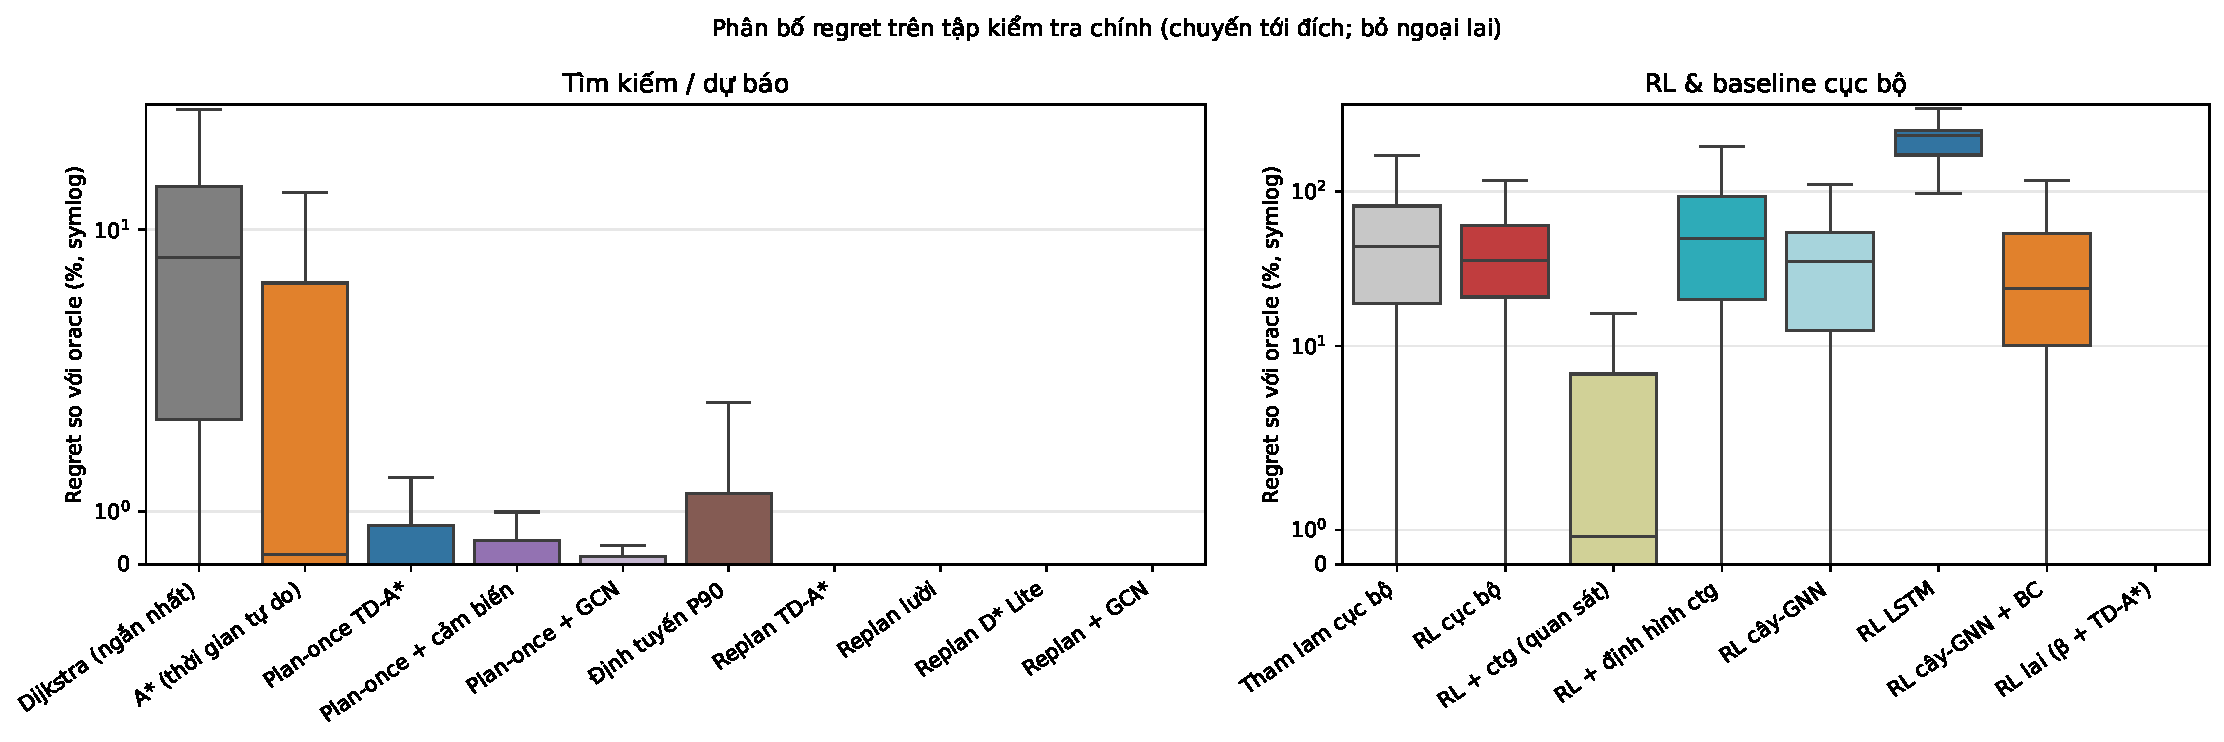
\includegraphics[width=\linewidth]{boxplot_methods.pdf}
\caption{Phân bố regret theo phương pháp trên tập kiểm tra chính (chuyến tới đích; trục tung dạng symlog).}
\label{fig:box}
\end{figure}

\textbf{Kiểm định thống kê} (Bảng~\ref{tab:tab_stat_tests}). Với mỗi cặp (A, B), chúng tôi báo cáo hiệu thời gian trung
bình $\bar{D}=\overline{T^A-T^B}$ (giá trị âm nghĩa là A nhanh hơn), khoảng tin cậy bootstrap 95\% \eqref{eq:bootstrap} và
giá trị $p$ của kiểm định Wilcoxon \eqref{eq:wilcoxon}:
\begin{itemize}
    \item Plan-once so với Dijkstra: $\bar{D}=\DiffPlanOnceDijkstraLength$ phút mỗi chuyến, khoảng tin cậy
    \CiPlanOnceDijkstraLength, $p$ \PPlanOnceDijkstraLength.
    \item Replan so với plan-once: $\bar{D}=\DiffReplanPlanOnce$ phút, khoảng tin cậy \CiReplanPlanOnce, $p$ \PReplanPlanOnce.
    \item Replan + GCN so với replan: $\bar{D}=\DiffReplanGnnReplan$ phút, khoảng tin cậy \CiReplanGnnReplan, $p$ \PReplanGnnReplan.
    \item Plan-once + GCN so với plan-once: $\bar{D}=\DiffPlanOnceGnnPlanOnce$ phút, khoảng tin cậy \CiPlanOnceGnnPlanOnce,
    $p$ \PPlanOnceGnnPlanOnce.
    \item Replan lười so với replan: $\bar{D}=\DiffReplanLazyReplan$ phút, khoảng tin cậy \CiReplanLazyReplan{} --- thực tế
    không khác biệt; D* Lite so với replan: $\bar{D}=\DiffReplanDstarReplan$ phút, khoảng tin cậy \CiReplanDstarReplan{} chứa 0.
    \item Định tuyến P90 so với plan-once: $\bar{D}=\DiffRiskPPlanOnce$ phút, khoảng tin cậy \CiRiskPPlanOnce, $p$
    \PRiskPPlanOnce{} --- định tuyến P90 hơi \emph{chậm hơn}.
\end{itemize}
Các khác biệt tính bằng phút là nhỏ vì phần lớn truy vấn không chịu ảnh hưởng của sự cố, nhưng nhất quán (khoảng tin cậy
không chứa 0) ở các cặp chính.

\begin{table}[!htbp]
\centering
\small
\caption{So sánh ghép cặp trên các truy vấn cả hai phương pháp cùng tới đích: khoảng tin cậy bootstrap 95\% của hiệu trung bình thời gian và kiểm định Wilcoxon signed-rank.}
\label{tab:tab_stat_tests}
\begin{adjustbox}{max width=\linewidth}
\begin{tabular}{lrrrrrrr}
\toprule
Cặp (A − B) & n & Hiệu TB (phút) & CI 95\% thấp & CI 95\% cao & Hiệu TB (\%) & A tốt hơn (\%) & p (Wilcoxon) \\
\midrule
Plan-once TD-A* − Dijkstra (ngắn nhất) & 200 & -1{,}499 & -1{,}738 & -1{,}270 & -7{,}974 & 78{,}000 & $<10^{-4}$ \\
Replan TD-A* − Plan-once TD-A* & 200 & -0{,}159 & -0{,}250 & -0{,}084 & -0{,}726 & 36{,}500 & $<10^{-4}$ \\
Oracle TD-A* − Replan TD-A* & 200 & -0{,}090 & -0{,}142 & -0{,}050 & -0{,}440 & 18{,}500 & $<10^{-4}$ \\
Replan lười − Replan TD-A* & 200 & 0{,}002 & 0{,}000 & 0{,}004 & 0{,}007 & 0{,}500 & 0{,}0687 \\
Replan D* Lite − Replan TD-A* & 200 & 0{,}015 & -0{,}036 & 0{,}077 & -0{,}020 & 3{,}500 & 0{,}3037 \\
Replan + GCN − Replan TD-A* & 200 & -0{,}048 & -0{,}105 & 0{,}005 & -0{,}250 & 10{,}500 & 0{,}0186 \\
Plan-once + cảm biến − Plan-once TD-A* & 200 & -0{,}081 & -0{,}155 & -0{,}013 & -0{,}316 & 16{,}000 & 0{,}0297 \\
Plan-once + GCN − Plan-once TD-A* & 200 & -0{,}124 & -0{,}199 & -0{,}055 & -0{,}635 & 26{,}000 & $<10^{-4}$ \\
Plan-once + GCN − Plan-once + cảm biến & 200 & -0{,}043 & -0{,}093 & 0{,}008 & -0{,}308 & 21{,}500 & 0{,}0002 \\
Định tuyến P90 − Plan-once TD-A* & 200 & 0{,}015 & -0{,}010 & 0{,}038 & 0{,}188 & 6{,}000 & 0{,}0027 \\
RL lai (β + TD-A*) − Replan TD-A* & 200 & 0{,}013 & 0{,}004 & 0{,}025 & 0{,}082 & 0{,}000 & 0{,}0009 \\
RL cây-GNN + BC − Plan-once TD-A* & 154 & 5{,}527 & 4{,}473 & 6{,}798 & 35{,}788 & 3{,}896 & $<10^{-4}$ \\
RL + ctg (quan sát) − A* (thời gian tự do) & 200 & -0{,}001 & -0{,}079 & 0{,}063 & 0{,}096 & 7{,}000 & 0{,}0002 \\
\bottomrule
\end{tabular}
\end{adjustbox}
\end{table}


\subsubsection{Chi phí tính toán}

Bảng~\ref{tab:tab_runtime_single} và Hình~\ref{fig:exp} so sánh chi phí tính toán đơn luồng. A* giảm \AstarReduction\% số nút
mở rộng so với Dijkstra. Với tìm kiếm phụ thuộc thời gian, heuristic chim bay chỉ giảm \TdAstarReduction\% so với TD-Dijkstra
vì phải chia cho $v_{\max}$ lớn (vận tốc tự do lớn nhất) trong khi vận tốc thực tế, nhất là giờ cao điểm, thấp hơn nhiều.
Heuristic cận dưới chính xác giảm \LbReduction\% (ít hơn heuristic chim bay \LbVsEuclid\%) nhưng tốn \LbPrep{} ms tiền xử lý
mỗi đích; ALT giảm \AltReduction\% với \AltPrep{} ms để tính heuristic mỗi truy vấn (tiền xử lý điểm mốc chỉ làm một lần).
TD-A* biên dịch Numba nhanh gấp \NumbaSpeedup{} lần bản Python với cùng số nút mở rộng. Replan tốn \RtRp{} ms mỗi chuyến
(\RpReplans{} lần tìm kiếm); replan lười nhanh gấp \LazySpeedup{} lần (\RpLazyReplans{} lần tìm kiếm); D* Lite nhanh gấp
\DstarSpeedup{} lần (\RpDstarExpanded{} nút mở rộng so với \RpExpanded{} của replan). Suy luận chính sách RL (PyTorch, từng
bước) tốn \RtRl{}--\RtRlTreeBc{} ms mỗi chuyến, chậm hơn TD-A* nhiều lần trên đồ thị cỡ này.

\begin{table}[!htbp]
\centering
\small
\caption{Chi phí tính toán đơn luồng (một tiến trình, tuần tự, 50 truy vấn kiểm tra, sau khi làm nóng). Với RL, cột nút mở rộng là số bước chính sách.}
\label{tab:tab_runtime_single}
\begin{adjustbox}{max width=\linewidth}
\begin{tabular}{lrrrr}
\toprule
Phương pháp & Nút mở rộng / bước TB & Thời gian TB (ms) & P90 (ms) & Tiền xử lý / truy vấn (ms) \\
\midrule
Dijkstra (ngắn nhất) & 1759 & 1{,}91 & 2{,}91 & -- \\
A* (ngắn nhất) & 524 & 0{,}65 & 1{,}39 & -- \\
A* (thời gian tự do) & 742 & 0{,}80 & 1{,}46 & -- \\
TD-Dijkstra (V\_base) & 1734 & 2{,}94 & 4{,}57 & -- \\
TD-A* (chim bay) = plan-once & 1101 & 1{,}77 & 3{,}03 & -- \\
TD-A* + heuristic LB & 498 & 0{,}83 & 1{,}88 & 3{,}24 \\
TD-A* + ALT & 884 & 1{,}36 & 2{,}83 & 1{,}55 \\
TD-A* (Numba) & 1101 & 0{,}32 & 0{,}50 & 0{,}00 \\
Oracle TD-A* & 1334 & 2{,}73 & 4{,}71 & -- \\
Plan-once + cảm biến & 1097 & 2{,}19 & 3{,}67 & -- \\
Plan-once + GCN & 1092 & 21{,}77 & 24{,}66 & -- \\
Định tuyến P90 & 1101 & 214{,}83 & 398{,}02 & -- \\
Replan TD-A* & 28424 & 53{,}16 & 123{,}52 & -- \\
Replan lười & 11996 & 27{,}10 & 67{,}91 & -- \\
Replan D* Lite & 2244 & 35{,}31 & 53{,}96 & -- \\
Replan + GCN & 27618 & 124{,}38 & 240{,}06 & -- \\
Tham lam cục bộ & 125 & 31{,}37 & 45{,}90 & -- \\
RL cục bộ & 121 & 75{,}85 & 120{,}16 & -- \\
RL + ctg (quan sát) & 47 & 43{,}51 & 53{,}69 & -- \\
RL + định hình ctg & 109 & 72{,}52 & 119{,}55 & -- \\
RL cây-GNN & 86 & 102{,}03 & 219{,}35 & -- \\
RL LSTM & 163 & 127{,}95 & 169{,}26 & -- \\
RL cây-GNN + BC & 86 & 108{,}22 & 215{,}29 & -- \\
RL lai (β + TD-A*) & 47 & 104{,}62 & 202{,}55 & -- \\
\bottomrule
\end{tabular}
\end{adjustbox}
\end{table}


\begin{figure}[H]
\centering
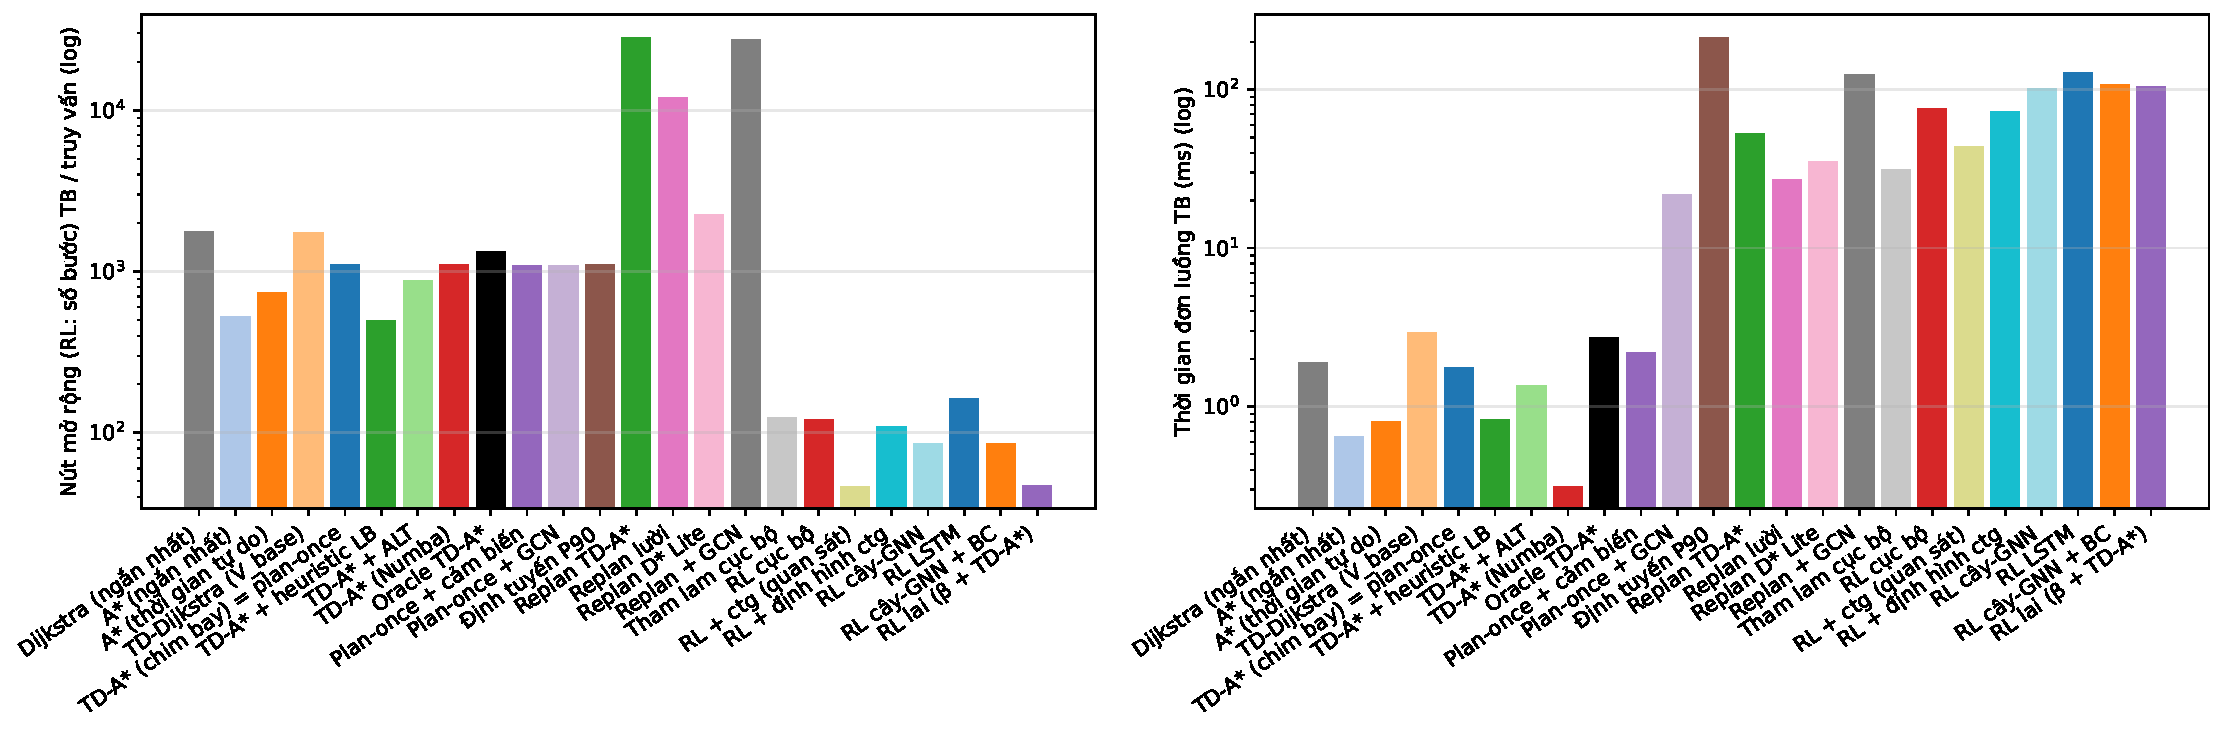
\includegraphics[width=\linewidth]{expansions_runtime.pdf}
\caption{Số nút mở rộng (trái) và thời gian tính đơn luồng (phải) trung bình mỗi truy vấn, thang logarit.}
\label{fig:exp}
\end{figure}

\subsubsection{Vai trò của sự cố và tập stress}

Theo số sự cố trên tập chính (Bảng~\ref{tab:tab_by_incidents}): khi không có sự cố, regret của plan-once chỉ \PoRegretZeroInc\%
và của replan \RpRegretZeroInc\%; với \MaxInc{} sự cố, các con số tương ứng là \PoRegretMaxInc\% và \RpRegretMaxInc\%. Trên tập
stress (Bảng~\ref{tab:tab_stress}), khi sự cố được đặt ưu tiên trên tuyến dự kiến, regret của plan-once tăng lên
\SPoRegret\% trong khi replan giữ \SRpRegret\% và replan + GCN \SRpGnnRegret\%; Dijkstra ngắn nhất \SDijRegret\%. Kết quả xác
nhận giả thuyết H2: tái lập kế hoạch có giá trị chủ yếu khi dự báo sai \emph{cục bộ và lớn}. Bảng~\ref{tab:tab_results_noinc}
cho thấy trên tập con không có sự cố, plan-once đã rất gần oracle, nên lợi ích của TD-A* so với Dijkstra là thật chứ không
do cách đặt sự cố.

\begin{table}[!htbp]
\centering
\small
\caption{Regret trung bình (\%) so với oracle theo số sự cố (chuyến tới đích).}
\label{tab:tab_by_incidents}
\begin{adjustbox}{max width=\linewidth}
\begin{tabular}{lrrrrrrrr}
\toprule
Nhóm & n & Dijkstra (ngắn nhất) & Plan-once TD-A* & Plan-once + GCN & Replan TD-A* & Replan + GCN & RL lai (β + TD-A*) & RL cây-GNN + BC \\
\midrule
0 & 81 & 10{,}48 & 0{,}83 & 0{,}37 & 0{,}35 & 0{,}17 & 0{,}44 & 38{,}50 \\
1 & 57 & 10{,}30 & 1{,}25 & 0{,}44 & 0{,}39 & 0{,}27 & 0{,}55 & 35{,}67 \\
2 & 38 & 12{,}04 & 1{,}16 & 1{,}10 & 0{,}53 & 0{,}25 & 0{,}53 & 35{,}52 \\
3 & 24 & 13{,}05 & 3{,}10 & 0{,}84 & 1{,}00 & 0{,}02 & 1{,}02 & 41{,}69 \\
\bottomrule
\end{tabular}
\end{adjustbox}
\end{table}

\begin{table}[!htbp]
\centering
\small
\caption{Kết quả trên tập stress (sự cố được ưu tiên đặt trên tuyến dự kiến với xác suất 0.7): cùng 200 truy vấn, cùng thời điểm/mức độ sự cố.}
\label{tab:tab_stress}
\begin{adjustbox}{max width=\linewidth}
\begin{tabular}{lrrrrrrrr}
\toprule
Phương pháp & Tới đích (\%) & TB (phút) & Trung vị & P90 & Regret TB (\%) & Regret TV (\%) & Regret P90 (\%) & Dài (km) \\
\midrule
Dijkstra (ngắn nhất) & 100{,}00 & 19{,}38 & 16{,}45 & 33{,}60 & 11{,}38 & 8{,}39 & 26{,}36 & 6{,}26 \\
A* (thời gian tự do) & 100{,}00 & 18{,}80 & 15{,}79 & 33{,}10 & 6{,}38 & 1{,}50 & 19{,}05 & 6{,}64 \\
Plan-once TD-A* & 100{,}00 & 18{,}10 & 15{,}47 & 31{,}84 & 3{,}37 & 0{,}23 & 11{,}44 & 6{,}62 \\
Plan-once + GCN & 100{,}00 & 17{,}88 & 15{,}46 & 31{,}84 & 2{,}10 & 0{,}00 & 5{,}99 & 6{,}58 \\
Định tuyến P90 & 100{,}00 & 18{,}11 & 15{,}56 & 31{,}85 & 3{,}51 & 0{,}52 & 11{,}73 & 6{,}63 \\
Replan TD-A* & 100{,}00 & 17{,}71 & 15{,}28 & 31{,}84 & 0{,}67 & 0{,}00 & 1{,}93 & 6{,}67 \\
Replan lười & 100{,}00 & 17{,}71 & 15{,}28 & 31{,}84 & 0{,}67 & 0{,}00 & 1{,}93 & 6{,}67 \\
Replan D* Lite & 100{,}00 & 17{,}72 & 15{,}28 & 31{,}84 & 0{,}66 & 0{,}00 & 2{,}20 & 6{,}65 \\
Replan + GCN & 100{,}00 & 17{,}64 & 15{,}14 & 31{,}84 & 0{,}31 & 0{,}00 & 0{,}28 & 6{,}64 \\
RL lai (β + TD-A*) & 100{,}00 & 17{,}73 & 15{,}28 & 31{,}84 & 0{,}80 & 0{,}00 & 2{,}33 & 6{,}66 \\
RL cây-GNN + BC & 77{,}50 & 21{,}91 & 18{,}53 & 38{,}82 & 40{,}77 & 26{,}96 & 75{,}24 & 7{,}64 \\
Oracle TD-A* & 100{,}00 & 17{,}57 & 15{,}02 & 31{,}71 & 0{,}00 & 0{,}00 & 0{,}00 & 6{,}66 \\
\bottomrule
\end{tabular}
\end{adjustbox}
\end{table}

\begin{table}[!htbp]
\centering
\small
\caption{Kết quả trên tập con kiểm tra không có sự cố (81 truy vấn).}
\label{tab:tab_results_noinc}
\begin{adjustbox}{max width=\linewidth}
\begin{tabular}{lrrrrrrrr}
\toprule
Phương pháp & Tới đích (\%) & TB (phút) & Trung vị & P90 & Regret TB (\%) & Regret TV (\%) & Regret P90 (\%) & Dài (km) \\
\midrule
Dijkstra (ngắn nhất) & 100{,}00 & 20{,}24 & 15{,}96 & 40{,}92 & 10{,}48 & 7{,}45 & 26{,}73 & 6{,}20 \\
A* (thời gian tự do) & 100{,}00 & 19{,}61 & 14{,}92 & 44{,}10 & 4{,}17 & 0{,}32 & 13{,}68 & 6{,}57 \\
Plan-once TD-A* & 100{,}00 & 18{,}66 & 14{,}77 & 38{,}74 & 0{,}83 & 0{,}00 & 2{,}62 & 6{,}57 \\
Plan-once + GCN & 100{,}00 & 18{,}57 & 14{,}39 & 37{,}68 & 0{,}37 & 0{,}00 & 0{,}97 & 6{,}49 \\
Replan TD-A* & 100{,}00 & 18{,}56 & 14{,}43 & 38{,}49 & 0{,}35 & 0{,}00 & 1{,}58 & 6{,}58 \\
Replan + GCN & 100{,}00 & 18{,}51 & 14{,}39 & 37{,}62 & 0{,}17 & 0{,}00 & 0{,}00 & 6{,}55 \\
RL lai (β + TD-A*) & 100{,}00 & 18{,}57 & 14{,}43 & 38{,}49 & 0{,}44 & 0{,}00 & 1{,}66 & 6{,}58 \\
Oracle TD-A* & 100{,}00 & 18{,}47 & 14{,}39 & 37{,}62 & 0{,}00 & 0{,}00 & 0{,}00 & 6{,}59 \\
\bottomrule
\end{tabular}
\end{adjustbox}
\end{table}


\subsubsection{Mức nhiễu, dự báo GCN và định tuyến P90}

GCN giảm RMSE \eqref{eq:rmse} của log-tỉ số vận tốc trên các cạnh chưa quan sát từ \GcnRmseZero{} (dự báo nền) xuống
\GcnRmse{}, tức giảm \GcnImprove\% (Bảng~\ref{tab:tab_forecast}, Hình~\ref{fig:gcn}). Lợi ích này chuyển thành chất lượng tuyến
và tăng theo mức nhiễu (Hình~\ref{fig:noise}, Bảng~\ref{tab:tab_noise_sweep}): với $\sigma=\NoiseMaxSigma$ và không có sự cố,
regret của plan-once là \NoisePoMax\%, plan-once + GCN \NoisePoGnnMax\%, replan \NoiseRpMax\%, replan + GCN \NoiseRpGnnMax\% và
Dijkstra \NoiseDijMax\%. Điều này chỉ xảy ra vì nhiễu có tương quan không gian--thời gian; với nhiễu độc lập (phiên bản đầu
của dự án) quan sát không mang thông tin về các cạnh khác nên không có gì để lan truyền.

\begin{table}[!htbp]
\centering
\small
\caption{Sai số dự báo log-tỉ số vận tốc (mốc $h$ và $h+1$) trên 20 trường kiểm định độc lập; 1341 cảm biến (15\% cạnh) + cạnh trong bán kính quan sát.}
\label{tab:tab_forecast}
\begin{adjustbox}{max width=\linewidth}
\begin{tabular}{lrr}
\toprule
Mô hình & RMSE cạnh chưa quan sát & RMSE mọi cạnh \\
\midrule
Dự báo nền V\_base (log-tỉ số = 0) & 0{,}1959 & 0{,}1965 \\
GCN chưa huấn luyện & 0{,}2375 & 0{,}2381 \\
GCN đã huấn luyện & 0{,}1602 & 0{,}1526 \\
\bottomrule
\end{tabular}
\end{adjustbox}
\end{table}


\begin{figure}[H]
\centering
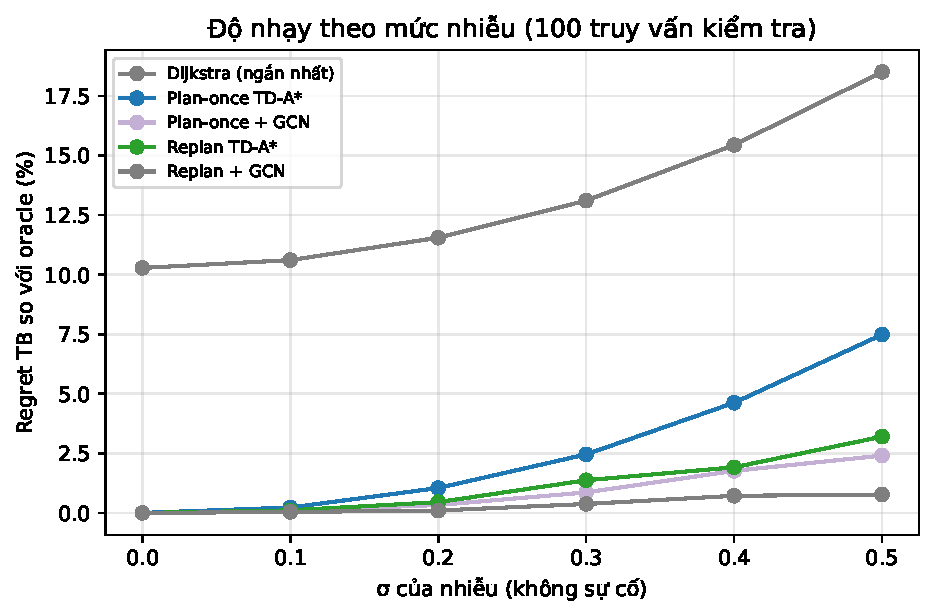
\includegraphics[width=0.49\linewidth]{noise_sensitivity.pdf}\hfill
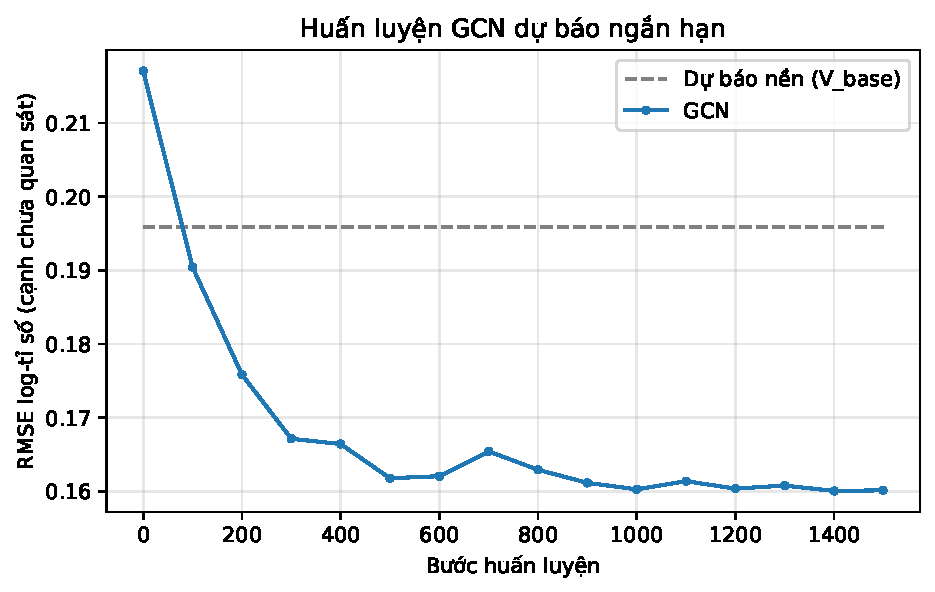
\includegraphics[width=0.49\linewidth]{gcn_training.pdf}
\caption{Trái: regret theo mức nhiễu $\sigma$ khi không có sự cố. Phải: RMSE trên cạnh chưa quan sát trong quá trình huấn
luyện GCN.}
\label{fig:noise}\label{fig:gcn}
\end{figure}

\begin{table}[!htbp]
\centering
\small
\caption{Regret trung bình (\%) theo mức nhiễu $\sigma$ khi không có sự cố.}
\label{tab:tab_noise_sweep}
\begin{adjustbox}{max width=\linewidth}
\begin{tabular}{lrrrrr}
\toprule
$\sigma$ & Dijkstra (ngắn nhất) & Plan-once TD-A* & Plan-once + GCN & Replan TD-A* & Replan + GCN \\
\midrule
0{,}00 & 10{,}28 & 0{,}00 & 0{,}00 & 0{,}00 & 0{,}00 \\
0{,}10 & 10{,}61 & 0{,}23 & 0{,}09 & 0{,}11 & 0{,}04 \\
0{,}20 & 11{,}55 & 1{,}05 & 0{,}33 & 0{,}45 & 0{,}10 \\
0{,}30 & 13{,}11 & 2{,}46 & 0{,}86 & 1{,}37 & 0{,}38 \\
0{,}40 & 15{,}44 & 4{,}62 & 1{,}77 & 1{,}92 & 0{,}72 \\
0{,}50 & 18{,}51 & 7{,}49 & 2{,}41 & 3{,}20 & 0{,}77 \\
\bottomrule
\end{tabular}
\end{adjustbox}
\end{table}


\textbf{Định tuyến P90 không mang lại lợi ích.} Trên \RiskEvalNQ{} truy vấn, mỗi tuyến được đánh giá trên 100 kịch bản độc
lập (Bảng~\ref{tab:tab_risk}). Tuyến P90 khác tuyến plan-once ở \RiskChangedPct\% số truy vấn, nhưng ở các truy vấn đó phân vị
90\% thực tế thay đổi trung bình \RiskDiffPnChanged{} phút (dương nghĩa là tệ hơn) và chỉ tốt hơn ở \RiskBetterPnPct\% số truy
vấn. Có hai nguyên nhân: (i) với $M=\RiskM$ kịch bản, phân vị ước lượng có sai số đáng kể, nên việc chọn ứng viên có phân vị
\emph{ước lượng} nhỏ nhất dẫn đến hiện tượng ``lời nguyền người thắng'' --- ứng viên được chọn thường là ứng viên được ước
lượng thấp hơn thực tế; (ii) trong mô phỏng, các tuyến ứng viên chồng lấp nhiều và nhiễu tương quan không gian khiến chúng
chịu rủi ro gần như nhau, nên không tồn tại tuyến ``an toàn'' rõ rệt.

\begin{table}[!htbp]
\centering
\small
\caption{Độ tin cậy tuyến trên 100 kịch bản nhiễu độc lập cho mỗi truy vấn (100 truy vấn kiểm tra, không sự cố). Tuyến P90 khác tuyến plan-once ở 20\% truy vấn.}
\label{tab:tab_risk}
\begin{adjustbox}{max width=\linewidth}
\begin{tabular}{lrrr}
\toprule
Tuyến & TB thời gian (phút) & P90 (phút) & Độ lệch chuẩn \\
\midrule
Plan-once TD-A* & 16{,}787 & 17{,}691 & 0{,}709 \\
Định tuyến P90 & 16{,}798 & 17{,}708 & 0{,}710 \\
\bottomrule
\end{tabular}
\end{adjustbox}
\end{table}


\subsubsection{Theo giờ xuất phát và khoảng cách}

Regret của tuyến ngắn nhất \emph{thấp hơn} vào giờ cao điểm (\DijRegretPeak\%) so với thấp điểm (\DijRegretOff\%)
(Bảng~\ref{tab:tab_by_peak}, Hình~\ref{fig:hour}). Phân tích tuyến nhanh nhất so với tuyến ngắn nhất trên vận tốc nền
(Hình~\ref{fig:saving}, Bảng~\ref{tab:tab_saving_by_hour}) xác nhận: tuyến nhanh nhất tiết kiệm \SavingThree\% lúc 3h nhưng chỉ
\SavingEight\% lúc 8h và \SavingEighteen\% lúc 18h. Nguyên nhân nằm ở mô hình: trục chính có độ nhạy và hệ số trục nóng cao
nhất nên vào cao điểm chậm gần bằng đường nhánh (Hình~\ref{fig:speedcurves}); lợi thế ``đi đường lớn dù xa hơn'' biến mất và
tuyến nhanh nhất hội tụ về tuyến ngắn. Đây là hệ quả của giả định mô phỏng và cần được kiểm chứng với dữ liệu thật; về
tuyệt đối, chuyến đi vẫn dài hơn nhiều vào cao điểm (tuyến ngắn nhất \TTShortEight{} phút lúc 8h so với \TTShortThree{} phút
lúc 3h). Theo khoảng cách (Bảng~\ref{tab:tab_by_distance}), regret tương đối của plan-once giảm khi chuyến đi dài hơn vì một
sự cố chiếm tỉ trọng nhỏ hơn trong tổng thời gian.

\begin{figure}[H]
\centering
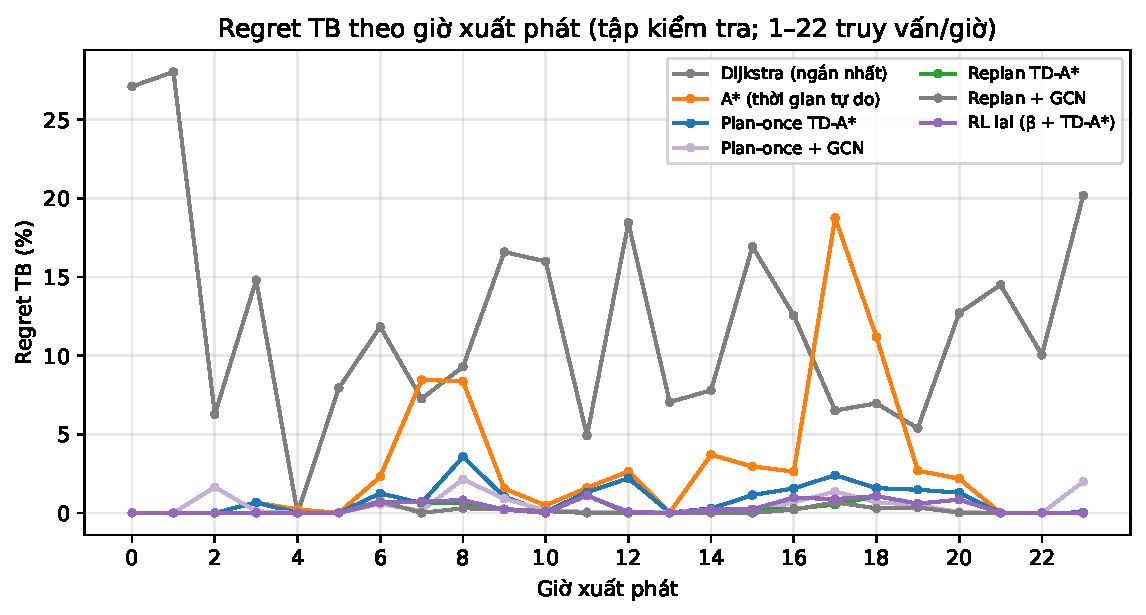
\includegraphics[width=0.49\linewidth]{regret_by_hour.pdf}\hfill
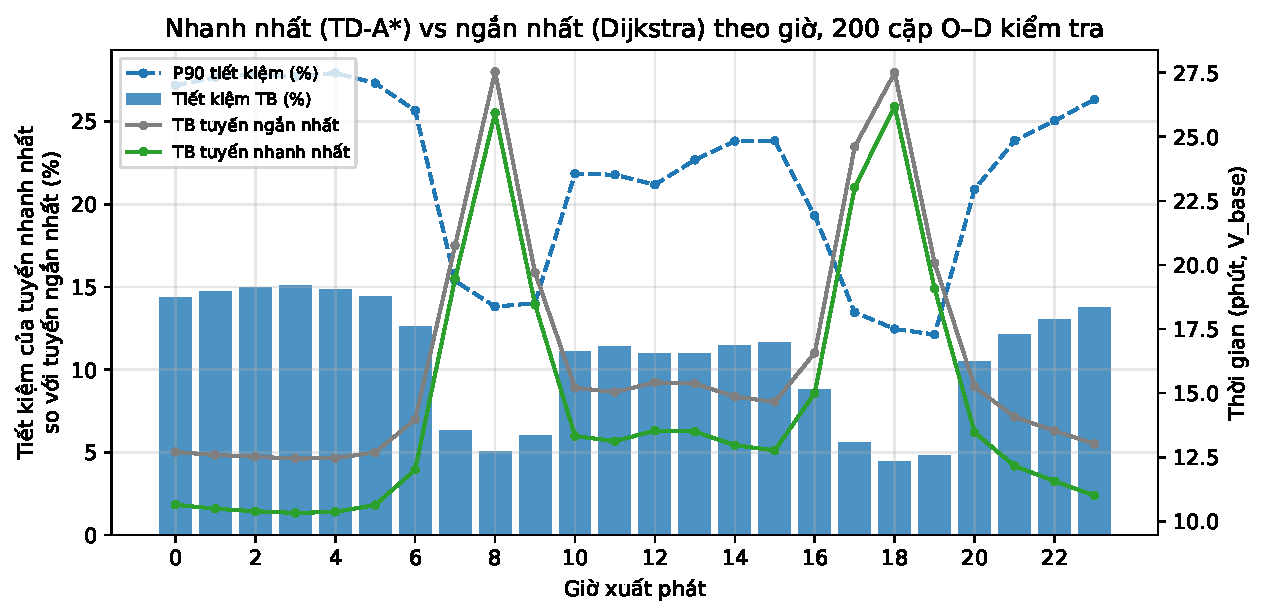
\includegraphics[width=0.49\linewidth]{saving_by_hour.pdf}
\caption{Trái: regret theo giờ xuất phát. Phải: tiết kiệm của tuyến nhanh nhất so với tuyến ngắn nhất theo giờ.}
\label{fig:hour}\label{fig:saving}
\end{figure}

\begin{table}[!htbp]
\centering
\small
\caption{Regret trung bình (\%) so với oracle theo giờ xuất phát (cao điểm: 7h, 8h, 17h, 18h) (chuyến tới đích).}
\label{tab:tab_by_peak}
\begin{adjustbox}{max width=\linewidth}
\begin{tabular}{lrrrrrrrr}
\toprule
Nhóm & n & Dijkstra (ngắn nhất) & Plan-once TD-A* & Plan-once + GCN & Replan TD-A* & Replan + GCN & RL lai (β + TD-A*) & RL cây-GNN + BC \\
\midrule
cao điểm & 74 & 7{,}46 & 1{,}91 & 0{,}98 & 0{,}76 & 0{,}29 & 0{,}88 & 28{,}20 \\
thấp điểm & 126 & 13{,}13 & 0{,}92 & 0{,}36 & 0{,}31 & 0{,}14 & 0{,}37 & 42{,}46 \\
\bottomrule
\end{tabular}
\end{adjustbox}
\end{table}

\begin{table}[!htbp]
\centering
\small
\caption{Regret trung bình (\%) so với oracle theo khoảng cách O–D (chuyến tới đích).}
\label{tab:tab_by_distance}
\begin{adjustbox}{max width=\linewidth}
\begin{tabular}{lrrrrrrrr}
\toprule
Nhóm & n & Dijkstra (ngắn nhất) & Plan-once TD-A* & Plan-once + GCN & Replan TD-A* & Replan + GCN & RL lai (β + TD-A*) & RL cây-GNN + BC \\
\midrule
ngan (<2.5km) & 42 & 10{,}18 & 1{,}39 & 0{,}34 & 0{,}31 & 0{,}11 & 0{,}48 & 37{,}09 \\
trung binh (2.5-4.5km) & 67 & 10{,}86 & 1{,}32 & 0{,}88 & 0{,}60 & 0{,}32 & 0{,}66 & 35{,}11 \\
xa (>4.5km) & 91 & 11{,}56 & 1{,}21 & 0{,}48 & 0{,}45 & 0{,}14 & 0{,}51 & 39{,}63 \\
\bottomrule
\end{tabular}
\end{adjustbox}
\end{table}

\begin{table}[!htbp]
\centering
\small
\caption{Regret trung bình (\%) so với oracle theo mức nhiễu $\sigma$ (chuyến tới đích).}
\label{tab:tab_by_sigma}
\begin{adjustbox}{max width=\linewidth}
\begin{tabular}{lrrrrrrrr}
\toprule
Nhóm & n & Dijkstra (ngắn nhất) & Plan-once TD-A* & Plan-once + GCN & Replan TD-A* & Replan + GCN & RL lai (β + TD-A*) & RL cây-GNN + BC \\
\midrule
0.05 & 76 & 10{,}84 & 0{,}46 & 0{,}54 & 0{,}04 & 0{,}04 & 0{,}04 & 36{,}15 \\
0.15 & 56 & 8{,}49 & 0{,}61 & 0{,}30 & 0{,}25 & 0{,}13 & 0{,}26 & 39{,}16 \\
0.3 & 68 & 13{,}34 & 2{,}77 & 0{,}88 & 1{,}14 & 0{,}41 & 1{,}38 & 37{,}38 \\
\bottomrule
\end{tabular}
\end{adjustbox}
\end{table}

\begin{table}[!htbp]
\centering
\small
\caption{Tiết kiệm thời gian của tuyến nhanh nhất so với tuyến ngắn nhất (trên vận tốc nền) theo giờ xuất phát.}
\label{tab:tab_saving_by_hour}
\begin{adjustbox}{max width=\linewidth}
\begin{tabular}{lrrrrr}
\toprule
Giờ & Ngắn nhất (phút) & Nhanh nhất (phút) & Tiết kiệm TB (\%) & P90 (\%) & Dài thêm (\%) \\
\midrule
0 & 12{,}70 & 10{,}64 & 14{,}38 & 27{,}19 & 6{,}1 \\
3 & 12{,}45 & 10{,}33 & 15{,}06 & 27{,}72 & 6{,}1 \\
6 & 13{,}96 & 12{,}01 & 12{,}61 & 25{,}67 & 5{,}4 \\
7 & 20{,}76 & 19{,}47 & 6{,}30 & 15{,}37 & 3{,}7 \\
8 & 27{,}53 & 25{,}93 & 5{,}06 & 13{,}81 & 3{,}9 \\
9 & 19{,}70 & 18{,}46 & 6{,}01 & 14{,}02 & 4{,}2 \\
12 & 15{,}42 & 13{,}54 & 10{,}96 & 21{,}18 & 4{,}9 \\
14 & 14{,}86 & 12{,}97 & 11{,}44 & 23{,}82 & 5{,}0 \\
16 & 16{,}57 & 15{,}00 & 8{,}81 & 19{,}31 & 4{,}1 \\
17 & 24{,}61 & 23{,}03 & 5{,}61 & 13{,}47 & 5{,}9 \\
18 & 27{,}50 & 26{,}18 & 4{,}45 & 12{,}46 & 6{,}0 \\
19 & 20{,}07 & 19{,}07 & 4{,}81 & 12{,}12 & 3{,}3 \\
21 & 14{,}07 & 12{,}16 & 12{,}15 & 23{,}83 & 5{,}3 \\
\bottomrule
\end{tabular}
\end{adjustbox}
\end{table}


\begin{figure}[H]
\centering
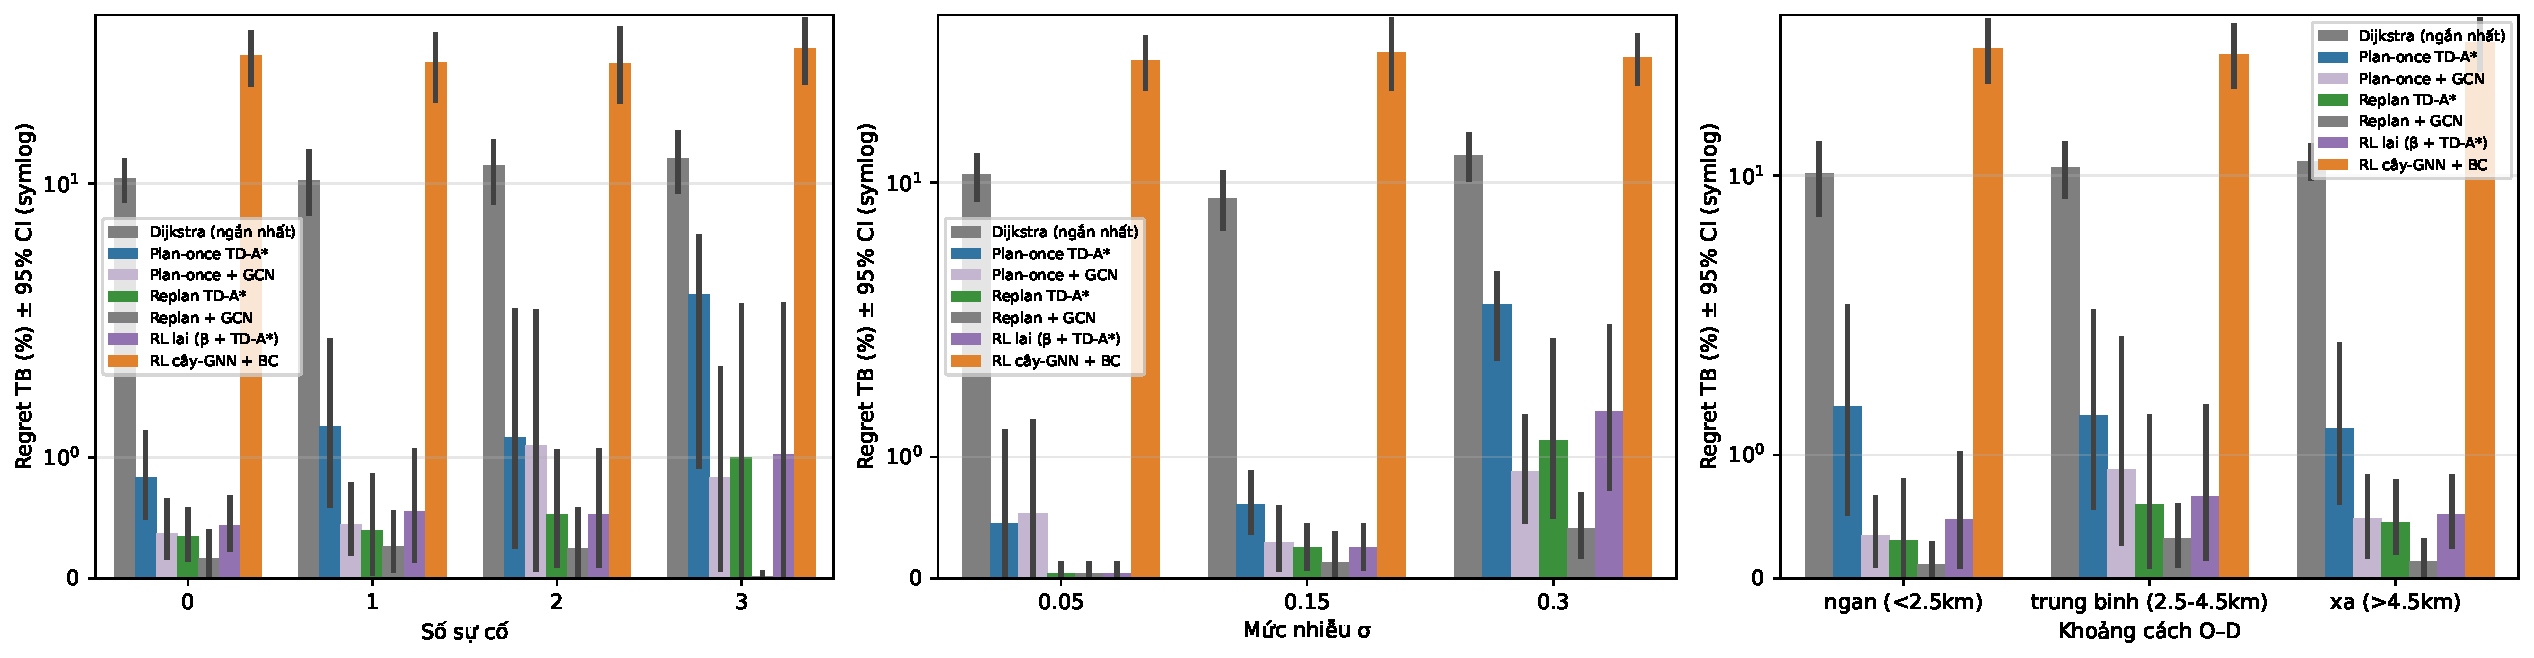
\includegraphics[width=\linewidth]{regret_breakdowns.pdf}
\caption{Regret theo số sự cố, mức nhiễu và khoảng cách (thanh lỗi: khoảng tin cậy bootstrap 95\%; trục symlog).}
\label{fig:breakdown}
\end{figure}

\subsubsection{Học tăng cường}

Bảng~\ref{tab:tab_main_rl} (seed tốt nhất theo tập kiểm định), Bảng~\ref{tab:tab_rl_seeds} (mọi seed) và Hình~\ref{fig:rl}
trình bày kết quả RL. Tỉ lệ tới đích trên tập kiểm tra, trung bình qua 3 seed: RL cục bộ \RlSeedSucc\%, RL + định hình ctg
\RlShapeSeedSucc\%, RL cây-GNN \RlTreeSeedSucc\%, RL cây-GNN + BC \RlTreeBcSeedSucc\%, RL LSTM \RlLstmSeedSucc\%; baseline tham
lam thủ công đạt \GrSuccess\%.

\begin{table}[!htbp]
\centering
\small
\caption{Kết quả các biến thể học tăng cường (seed tốt nhất theo tập kiểm định) và baseline tham lam trên cùng tập kiểm tra; thời gian và regret chỉ tính trên các chuyến tới đích.}
\label{tab:tab_main_rl}
\begin{adjustbox}{max width=\linewidth}
\begin{tabular}{lrrrrrrrr}
\toprule
Phương pháp & Tới đích (\%) & TB (phút) & Trung vị & P90 & Regret TB (\%) & Regret TV (\%) & Regret P90 (\%) & Dài (km) \\
\midrule
Tham lam cục bộ & 37{,}50 & 21{,}02 & 17{,}56 & 38{,}70 & 62{,}88 & 43{,}80 & 135{,}28 & 6{,}75 \\
RL cục bộ & 35{,}00 & 22{,}27 & 18{,}83 & 42{,}88 & 63{,}24 & 35{,}74 & 90{,}16 & 7{,}17 \\
RL + ctg (quan sát) & 100{,}00 & 18{,}32 & 15{,}23 & 31{,}52 & 5{,}19 & 0{,}82 & 17{,}79 & 6{,}64 \\
RL + định hình ctg & 57{,}00 & 24{,}18 & 20{,}50 & 43{,}68 & 76{,}11 & 49{,}93 & 183{,}88 & 7{,}87 \\
RL cây-GNN & 67{,}00 & 20{,}55 & 18{,}60 & 35{,}43 & 39{,}38 & 35{,}44 & 87{,}93 & 7{,}31 \\
RL LSTM & 2{,}50 & 22{,}83 & 23{,}23 & 29{,}17 & 219{,}06 & 230{,}42 & 307{,}75 & 6{,}36 \\
RL cây-GNN + BC & 77{,}00 & 21{,}59 & 17{,}74 & 40{,}35 & 37{,}36 & 23{,}74 & 73{,}33 & 7{,}57 \\
RL lai (β + TD-A*) & 100{,}00 & 17{,}37 & 14{,}47 & 30{,}89 & 0{,}56 & 0{,}00 & 1{,}67 & 6{,}63 \\
Replan TD-A* & 100{,}00 & 17{,}35 & 14{,}47 & 30{,}89 & 0{,}47 & 0{,}00 & 1{,}18 & 6{,}63 \\
Oracle TD-A* & 100{,}00 & 17{,}26 & 14{,}47 & 30{,}89 & 0{,}00 & 0{,}00 & 0{,}00 & 6{,}64 \\
\bottomrule
\end{tabular}
\end{adjustbox}
\end{table}


\begin{figure}[H]
\centering
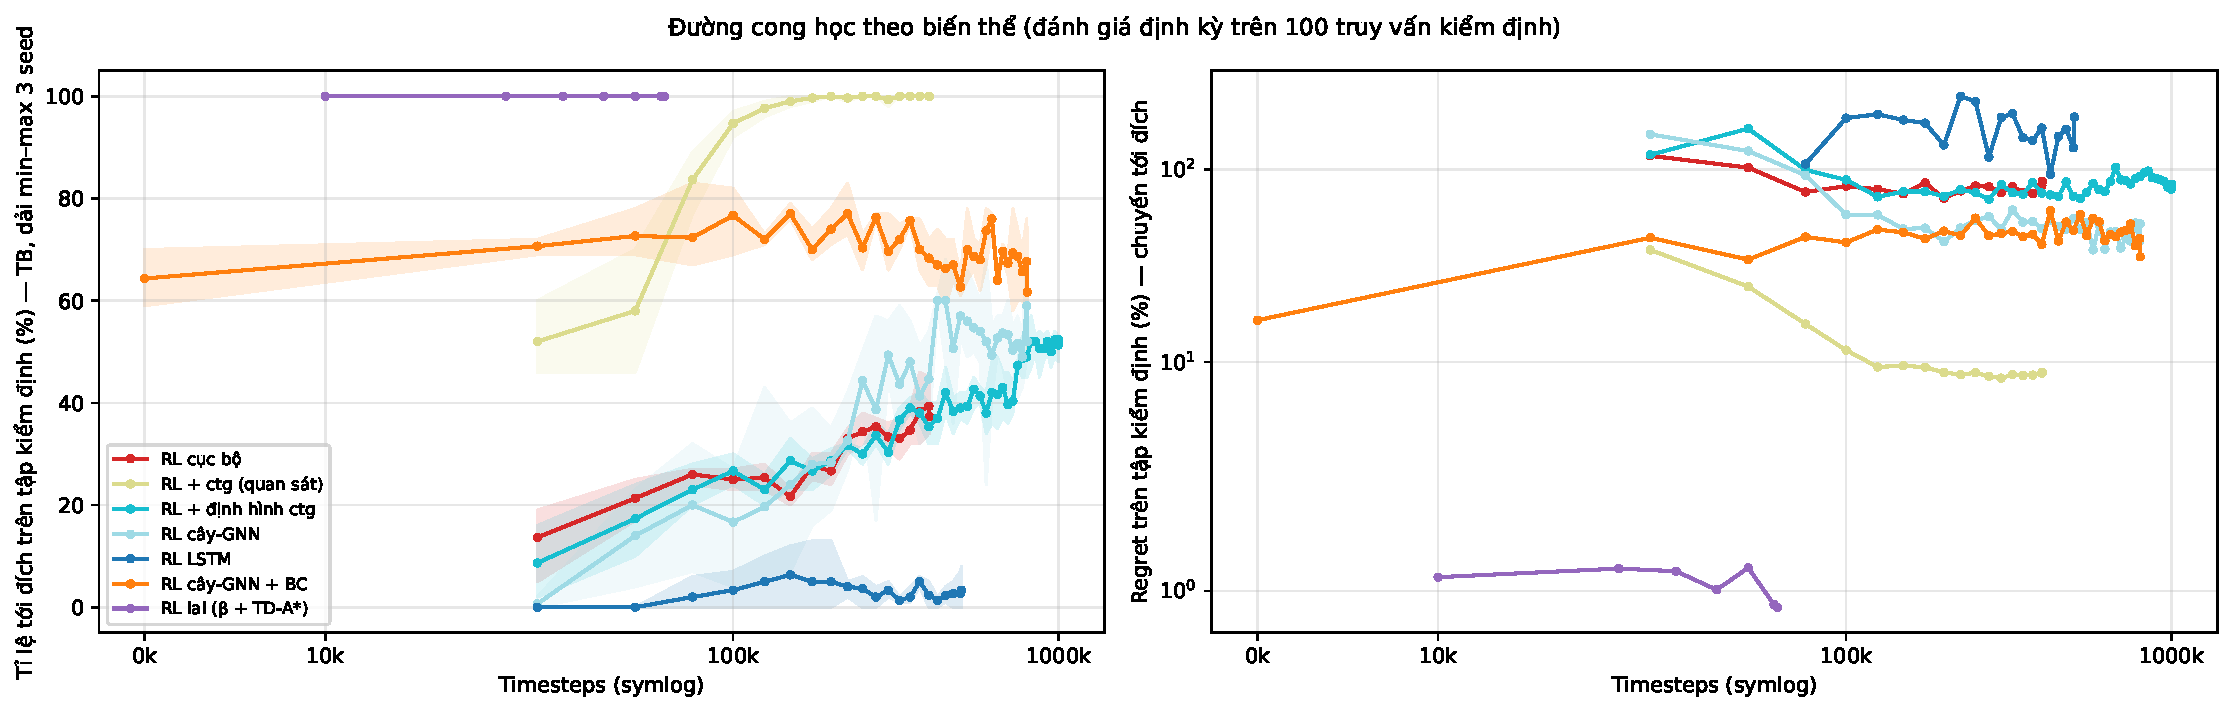
\includegraphics[width=\linewidth]{rl_learning_curves.pdf}
\caption{Đường cong học trên tập kiểm định: trung bình và dải min--max qua 3 seed (trục hoành symlog).}
\label{fig:rl}
\end{figure}

\textbf{Cải tiến nào có tác dụng?}
\begin{itemize}
    \item \emph{Quan sát rộng hơn có tác dụng lớn nhất trong nhóm chọn từng cạnh.} Cây lân cận \TreeDepth{} bước với GNN nâng
    tỉ lệ tới đích từ \RlSuccess\% lên \RlTreeSuccess\% và giảm regret từ \RlRegret\% xuống \RlTreeRegret\%: tác tử nhìn thấy ngõ
    cụt phía trước (\DeadEndPct\% số nút là ngõ cụt) thay vì chỉ thấy hướng chim bay. Đường cong học vẫn đang đi lên ở cuối ngân
    sách, nên huấn luyện lâu hơn có thể còn cải thiện.
    \item \emph{Học bắt chước cho kết quả tốt nhất.} Chỉ riêng giai đoạn BC đã đạt độ chính xác bắt chước \RlTreeBcBcAcc\% và
    \RlTreeBcAfterBc\% tới đích trên tập kiểm định (trung bình 3 seed) trước khi chạy PPO; seed được chọn đạt \RlTreeBcSuccess\%
    trên tập kiểm tra (regret \RlTreeBcRegret\%). Tuy nhiên PPO tinh chỉnh \emph{không} cải thiện thêm mà làm chính sách dao động
    và giảm dần (Hình~\ref{fig:rl}); checkpoint tốt nhất thường xuất hiện sớm. Đây là hiện tượng thường gặp khi tinh chỉnh bằng
    gradient chính sách với phần thưởng thưa sau giai đoạn bắt chước.
    \item \emph{Định hình theo cost-to-go} tăng tỉ lệ tới đích (\RlShapeSuccess\% so với \RlSuccess\%) nhưng regret trên các
    chuyến tới đích không giảm (\RlShapeRegret\%): định hình chỉ hướng tác tử về đích mà không dạy nó tránh đoạn chậm.
    \item \emph{Bộ nhớ LSTM thất bại} (\RlLstmSuccess\%): RecurrentPPO không có mặt nạ hành động nên phải ánh xạ $a\bmod\deg^+(u)$,
    làm ý nghĩa của mỗi đầu ra thay đổi theo bậc của nút; cộng với tốc độ học chậm hơn nhiều, chính sách không thoát khỏi việc
    đi lòng vòng.
    \item \emph{Thí nghiệm đối chứng có thông tin toàn cục} (cost-to-go trong quan sát) tới đích \RlcSuccess\% với regret
    \RlcRegret\%, nhưng tuyến của nó trùng hệt tuyến A* thời gian tự do ở \RouteSameRlcFf\% số truy vấn và thời gian không khác
    biệt so với A* tự do (Bảng~\ref{tab:tab_stat_tests}): chính sách chủ yếu bám theo gradient của cost-to-go tĩnh.
    \item \emph{RL lai đạt 100\% tới đích với regret \RlHybRegret\%} nhưng không vượt được replan thuần (\RpRegret\%): hiệu
    \DiffRlHybridReplan{} phút mỗi chuyến, khoảng tin cậy \CiRlHybridReplan, Wilcoxon $p$ \PRlHybridReplan. Tác tử học được
    $\bar\beta=\HybMeanBeta$, gần với $\beta=1$ của replan, và tuyến trùng replan ở \RouteSameRlHybRp\% số truy vấn. Giá trị của RL
    ở đây là \emph{giữ được} bảo đảm tới đích và chất lượng của tìm kiếm, chứ chưa tạo thêm lợi ích.
\end{itemize}
Mọi biến thể RL chọn từng cạnh vẫn kém plan-once rất xa: biến thể tốt nhất (cây-GNN + BC) chậm hơn plan-once
\DiffRlTreeBcPlanOnce{} phút mỗi chuyến trên các truy vấn nó tới đích (\CiRlTreeBcPlanOnce) và chỉ tốt hơn ở
\BetterRlTreeBcPlanOnce\% số truy vấn. Kết quả xác nhận giả thuyết H3.

\begin{table}[!htbp]
\centering
\small
\caption{Kết quả học tăng cường theo từng seed (checkpoint tốt nhất theo tập kiểm định; cột Chọn đánh dấu seed dùng cho bảng chính).}
\label{tab:tab_rl_seeds}
\begin{adjustbox}{max width=\linewidth}
\begin{tabular}{lrrrrrrrc}
\toprule
Biến thể & Seed & Bước & Val tới đích (\%) & Tốt nhất tại & Test tới đích (\%) & Test regret (\%) & Huấn luyện (phút) & Chọn \\
\midrule
RL cục bộ & 0 & 401408 & 46{,}0 & 375000 & 35{,}0 & 63{,}24 & 21{,}5 & x \\
RL cục bộ & 1 & 401408 & 39{,}0 & 400000 & 37{,}0 & 62{,}18 & 19{,}4 &  \\
RL cục bộ & 2 & 401408 & 37{,}0 & 375000 & 38{,}0 & 66{,}14 & 19{,}8 &  \\
RL + ctg (quan sát) & 0 & 401408 & 100{,}0 & 275000 & 99{,}0 & 5{,}34 & 21{,}1 &  \\
RL + ctg (quan sát) & 1 & 401408 & 100{,}0 & 400000 & 100{,}0 & 5{,}19 & 21{,}1 & x \\
RL + ctg (quan sát) & 2 & 401408 & 100{,}0 & 300000 & 99{,}5 & 5{,}16 & 14{,}9 &  \\
RL + định hình ctg & 0 & 1003520 & 57{,}0 & 825000 & 57{,}0 & 76{,}11 & 50{,}7 & x \\
RL + định hình ctg & 1 & 1003520 & 52{,}0 & 925000 & 49{,}5 & 63{,}25 & 50{,}6 &  \\
RL + định hình ctg & 2 & 1003520 & 53{,}0 & 1000000 & 58{,}5 & 72{,}94 & 51{,}4 &  \\
RL cây-GNN & 0 & 802816 & 68{,}0 & 600000 & 67{,}0 & 39{,}38 & 153{,}9 & x \\
RL cây-GNN & 1 & 802816 & 65{,}0 & 475000 & 74{,}0 & 54{,}33 & 153{,}5 &  \\
RL cây-GNN & 2 & 802816 & 60{,}0 & 800000 & 63{,}0 & 42{,}31 & 155{,}5 &  \\
RL LSTM & 0 & 503808 & 1{,}0 & 450000 & 2{,}5 & 219{,}06 & 169{,}7 & x \\
RL LSTM & 1 & 503808 & 13{,}0 & 175000 & 8{,}5 & 175{,}38 & 138{,}6 &  \\
RL LSTM & 2 & 503808 & 2{,}0 & 425000 & 1{,}0 & 280{,}42 & 138{,}5 &  \\
RL cây-GNN + BC & 0 & 802816 & 82{,}0 & 100000 & 77{,}0 & 37{,}36 & 160{,}7 & x \\
RL cây-GNN + BC & 1 & 802816 & 83{,}0 & 225000 & 86{,}0 & 42{,}94 & 160{,}9 &  \\
RL cây-GNN + BC & 2 & 802816 & 77{,}0 & 625000 & 76{,}5 & 45{,}54 & 161{,}2 &  \\
RL lai (β + TD-A*) & 0 & 61440 & 100{,}0 & 30000 & 100{,}0 & 0{,}56 & 11{,}5 & x \\
RL lai (β + TD-A*) & 1 & 61440 & 100{,}0 & 61440 & 100{,}0 & 0{,}90 & 11{,}4 &  \\
RL lai (β + TD-A*) & 2 & 61440 & 100{,}0 & 60000 & 100{,}0 & 0{,}50 & 11{,}2 &  \\
\bottomrule
\end{tabular}
\end{adjustbox}
\end{table}

\begin{table}[!htbp]
\centering
\small
\caption{Độ trùng tuyến giữa các cặp phương pháp trên tập kiểm tra chính.}
\label{tab:tab_route_overlap}
\begin{adjustbox}{max width=\linewidth}
\begin{tabular}{lrrr}
\toprule
Cặp phương pháp & n & Tuyến giống hệt (\%) & Jaccard cạnh TB (\%) \\
\midrule
RL + ctg (quan sát) vs A* (thời gian tự do) & 200 & 64{,}0 & 91{,}7 \\
RL cây-GNN + BC vs Oracle TD-A* & 200 & 3{,}5 & 32{,}1 \\
RL cây-GNN + BC vs Plan-once TD-A* & 200 & 2{,}5 & 31{,}6 \\
RL lai (β + TD-A*) vs Replan TD-A* & 200 & 93{,}5 & 98{,}1 \\
Plan-once TD-A* vs Oracle TD-A* & 200 & 57{,}5 & 84{,}1 \\
Replan TD-A* vs Oracle TD-A* & 200 & 81{,}5 & 91{,}0 \\
Replan lười vs Replan TD-A* & 200 & 96{,}0 & 99{,}1 \\
Replan D* Lite vs Replan TD-A* & 200 & 88{,}0 & 94{,}9 \\
Replan + GCN vs Replan TD-A* & 200 & 86{,}5 & 92{,}2 \\
Định tuyến P90 vs Plan-once TD-A* & 200 & 77{,}5 & 94{,}6 \\
A* (thời gian tự do) vs Dijkstra (ngắn nhất) & 200 & 12{,}5 & 47{,}1 \\
\bottomrule
\end{tabular}
\end{adjustbox}
\end{table}


\begin{figure}[H]
\centering
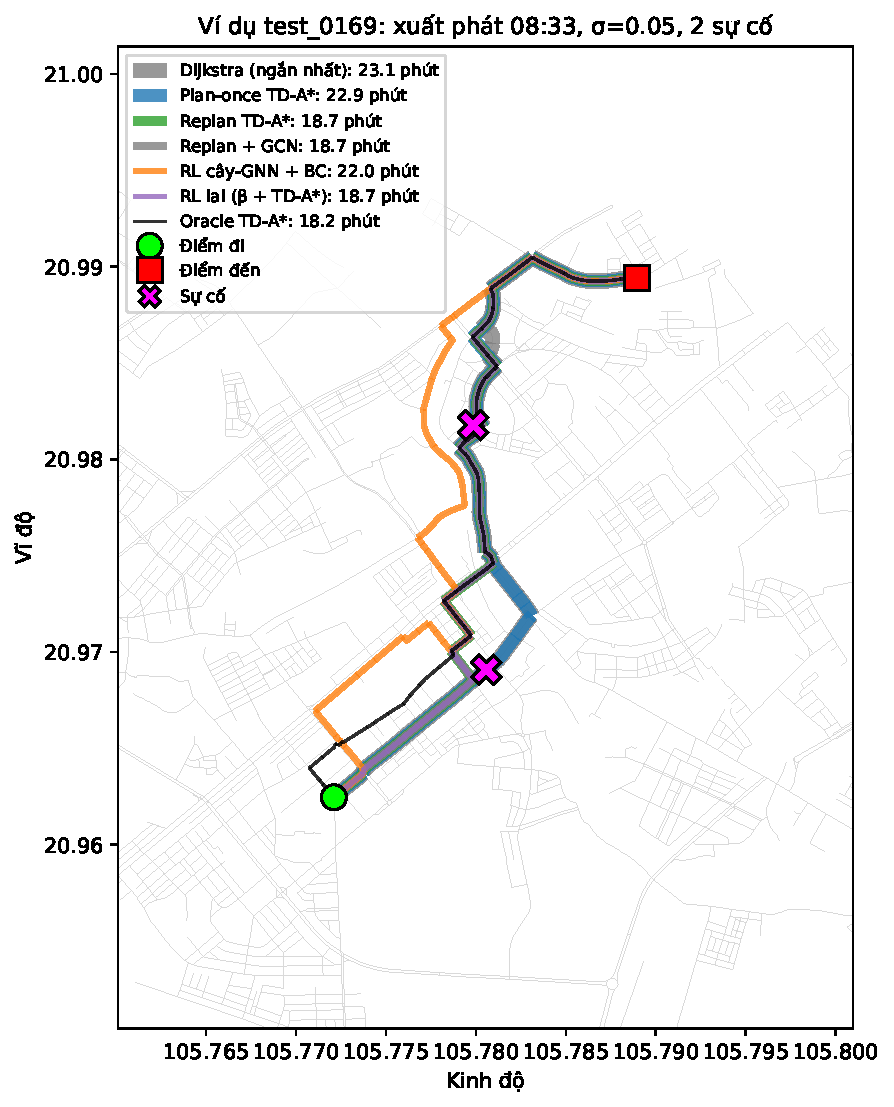
\includegraphics[width=0.66\linewidth]{route_example.pdf}
\caption{Ví dụ truy vấn \ExampleQuery{} (truy vấn có sự cố với chênh lệch giữa plan-once và replan lớn nhất).}
\label{fig:route}
\end{figure}

\subsubsection{Chọn giờ xuất phát}

Bảng~\ref{tab:tab_departure} và Hình~\ref{fig:dep} trình bày kết quả. Khi tính đủ thời gian chờ ($w=1$), chờ không bao giờ
có lợi trên tập kiểm tra (lời giải vét cạn chọn chờ ở \DepOptWOneWait\% số truy vấn) và Q-learning học đúng chính sách ``đi
ngay''. Khi chờ rẻ hơn ($w=\DepLowW$), lời giải vét cạn chọn chờ ở \DepOptWLowWait\% số truy vấn và giảm chi phí trung bình
từ \DepGoWLowCost{} xuống \DepOptWLowCost{} phút --- có truy vấn tiết kiệm tới \DepMaxSaving{} phút nhờ tránh cao điểm --- nhưng
Q-learning dạng bảng \emph{không} nhận diện được các truy vấn đó: chi phí \DepQWLowCost{} phút, regret \DepQWLowRegret{} phút
so với \DepGoWLowRegret{} phút của ``đi ngay''. Trong lần chạy đầu, việc khởi tạo $Q=0$ (lạc quan vì mọi phần thưởng đều âm)
khiến tác tử chờ quá nhiều ở các trạng thái hiếm gặp; quy tắc chỉ tin $Q$ ở ô đã cập nhật đủ \DepMinVisits{} lần
(Mục~\ref{sec:method:departure}) đã khắc phục phần lớn vấn đề này.

\begin{table}[!htbp]
\centering
\small
\caption{Kết quả thí nghiệm chọn giờ xuất phát trên tập kiểm tra (bước chờ 10 phút, tối đa 6 lần).}
\label{tab:tab_departure}
\begin{adjustbox}{max width=\linewidth}
\begin{tabular}{llrrrrr}
\toprule
w & Chính sách & Chi phí TB (phút) & Đi TB (phút) & Chờ+đi TB (phút) & Tỉ lệ chờ & Regret (phút) \\
\midrule
0{,}25 & Đi ngay & 17{,}26 & 17{,}26 & 17{,}26 & 0{,}000 & 0{,}183 \\
0{,}25 & Giờ tối ưu (vét cạn) & 17{,}08 & 16{,}62 & 18{,}47 & 0{,}050 & 0{,}000 \\
0{,}25 & Q-learning & 17{,}73 & 16{,}75 & 20{,}65 & 0{,}160 & 0{,}649 \\
0{,}50 & Đi ngay & 17{,}26 & 17{,}26 & 17{,}26 & 0{,}000 & 0{,}007 \\
0{,}50 & Giờ tối ưu (vét cạn) & 17{,}26 & 17{,}18 & 17{,}33 & 0{,}010 & 0{,}000 \\
0{,}50 & Q-learning & 17{,}55 & 17{,}10 & 18{,}00 & 0{,}060 & 0{,}294 \\
1{,}00 & Đi ngay & 17{,}26 & 17{,}26 & 17{,}26 & 0{,}000 & 0{,}000 \\
1{,}00 & Giờ tối ưu (vét cạn) & 17{,}26 & 17{,}26 & 17{,}26 & 0{,}000 & 0{,}000 \\
1{,}00 & Q-learning & 17{,}26 & 17{,}26 & 17{,}26 & 0{,}000 & 0{,}000 \\
\bottomrule
\end{tabular}
\end{adjustbox}
\end{table}


\begin{figure}[H]
\centering
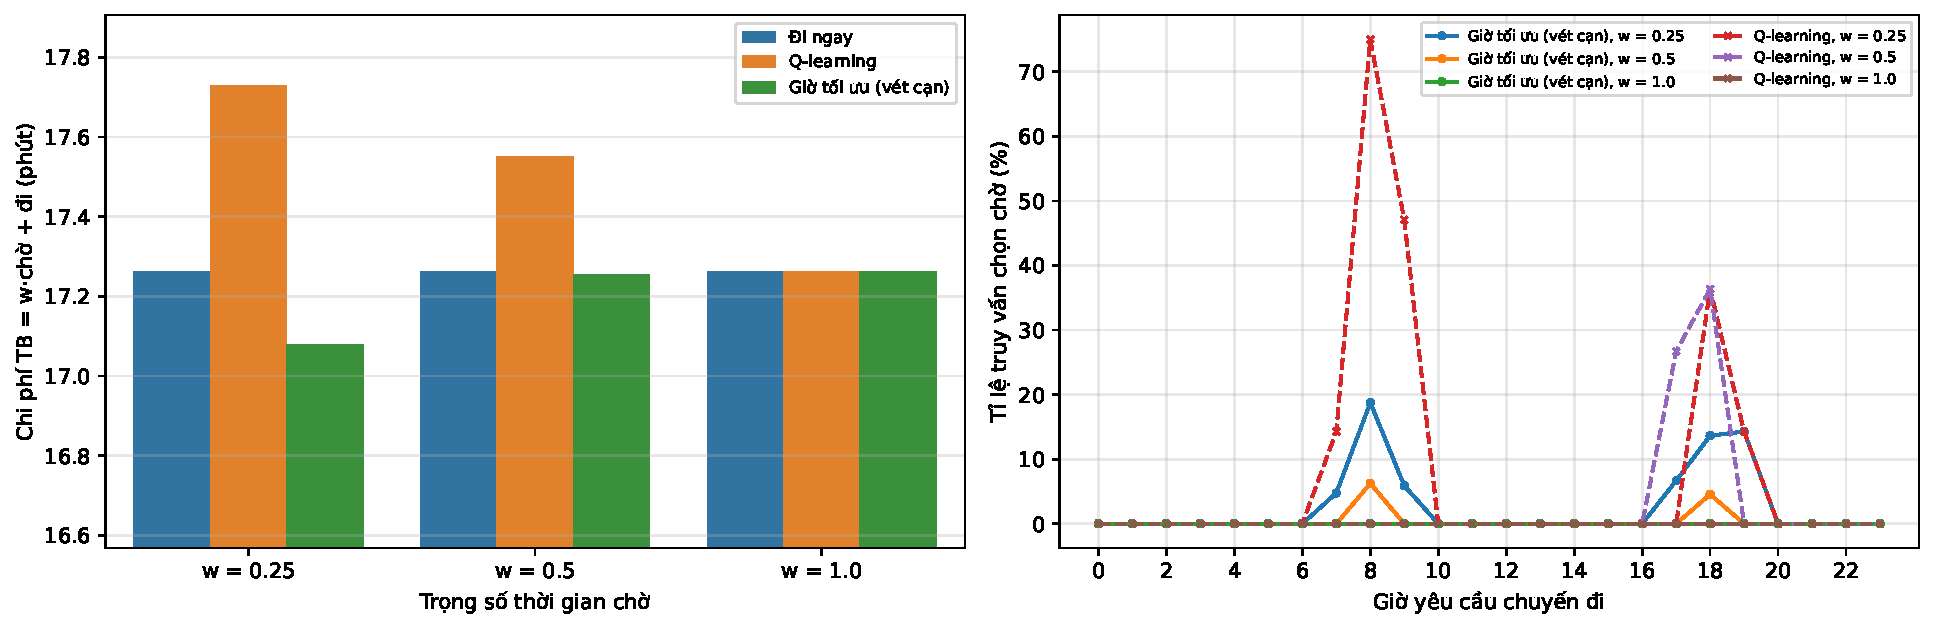
\includegraphics[width=\linewidth]{departure_time.pdf}
\caption{Chọn giờ xuất phát: chi phí trung bình theo chính sách (trái) và tỉ lệ chọn chờ theo giờ (phải).}
\label{fig:dep}
\end{figure}

\subsubsection{Nhiều xe cùng được dẫn đường}

Khi \MaVeh{} xe khởi hành trong khung 7:30--8:00 cùng làm theo một chỉ dẫn TD-A* trên dự báo, thời gian đi trung bình tăng từ
\MaFree{} phút (nếu các xe không ảnh hưởng nhau) lên \MaNaive{} phút, tức tăng \MaNaiveInc\% (Bảng~\ref{tab:tab_multiagent},
Hình~\ref{fig:ma}): tải dồn vào cùng các trục ``nhanh nhất'' với tỉ số lưu lượng/năng lực lớn nhất tới \MaVcNaive. Phối hợp tuần
tự (mỗi xe thấy tải của các xe đã lập trước) giảm thời gian còn \MaCoord{} phút, tốt hơn \MaCoordGain\% so với dẫn đường giống
nhau. Kết quả xác nhận giả thuyết H4: dẫn đường cá nhân tối ưu có thể làm hệ thống tệ đi khi tỉ lệ xe dùng nó lớn, và cần phân
bổ có tính đến tải (cân bằng Wardrop~\cite{wardrop1952} hoặc tối ưu hệ thống).

\begin{table}[!htbp]
\centering
\small
\caption{Thời gian đi trung bình (phút) khi nhiều xe được dẫn đường cùng lúc; V/C là tỉ số lớn nhất giữa lưu lượng dẫn đường và năng lực.}
\label{tab:tab_multiagent}
\begin{adjustbox}{max width=\linewidth}
\begin{tabular}{lrrrrr}
\toprule
Số xe & Không tương tác & Naive & Phối hợp & V/C max (naive) & V/C max (phối hợp) \\
\midrule
1000 & 28{,}45 & 29{,}26 & 29{,}18 & 0{,}80 & 0{,}80 \\
2000 & 28{,}52 & 31{,}35 & 30{,}69 & 2{,}13 & 1{,}87 \\
4000 & 27{,}78 & 31{,}49 & 30{,}38 & 2{,}67 & 1{,}87 \\
8000 & 27{,}45 & 34{,}83 & 32{,}56 & 4{,}53 & 2{,}40 \\
16000 & 27{,}04 & 43{,}46 & 36{,}80 & 8{,}00 & 3{,}20 \\
\bottomrule
\end{tabular}
\end{adjustbox}
\end{table}


\begin{figure}[H]
\centering
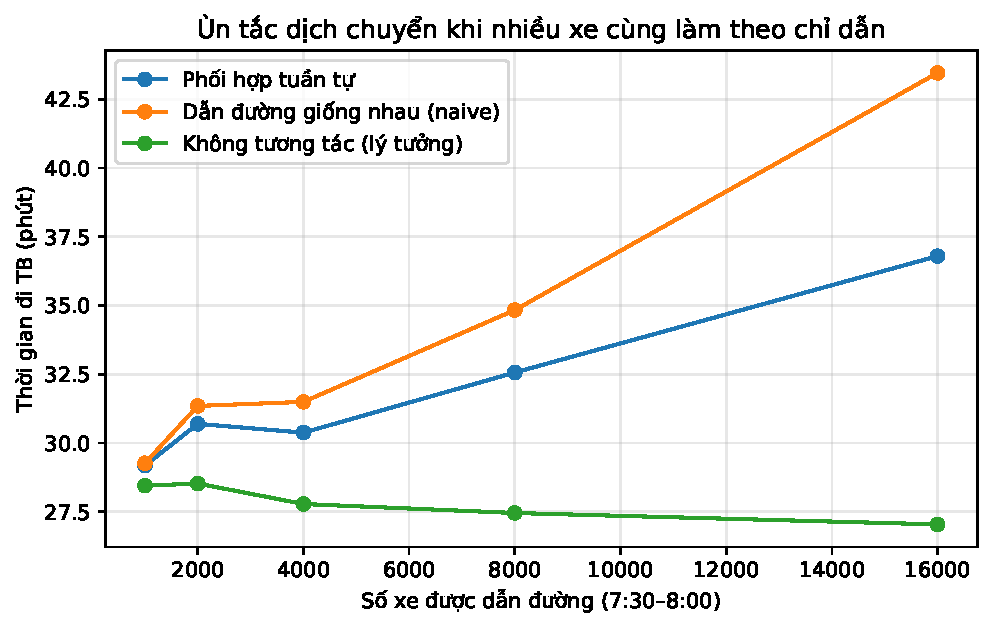
\includegraphics[width=0.66\linewidth]{multiagent.pdf}
\caption{Thời gian đi trung bình theo số xe được dẫn đường cùng lúc.}
\label{fig:ma}
\end{figure}

\subsubsection{Khi nào phương pháp đề xuất tốt hơn, và tại sao}

\begin{enumerate}[label=(\arabic*)]
    \item \textbf{TD-A* thay cho tuyến tĩnh} luôn có lợi khi vận tốc biến thiên theo giờ: regret giảm từ \DijRegret\% xuống
    \PoRegret\%. Lợi ích tương đối nhỏ hơn vào cao điểm vì trong mô hình mọi trục đều tắc.
    \item \textbf{Replan} có lợi khi dự báo sai cục bộ và lớn (sự cố, nhiễu cao); khi dự báo tốt, plan-once đã gần tối ưu.
    \textbf{Replan lười} cho cùng chất lượng và nhanh gấp \LazySpeedup{} lần; \textbf{D* Lite} nhanh hơn nhưng dùng chi phí
    snapshot nên có thể lệch nhẹ --- trên đồ thị cỡ này mọi biến thể đều đủ nhanh cho ứng dụng tương tác.
    \item \textbf{Dự báo GCN} có lợi khi nhiễu có tương quan không gian--thời gian và có mạng cảm biến: replan + GCN là phương
    pháp tốt nhất (\RpGnnRegret\%), và lợi ích tăng theo mức nhiễu. Với nhiễu độc lập, không có gì để lan truyền.
    \item \textbf{Định tuyến P90} không có lợi trong mô phỏng này do ước lượng phân vị từ ít mẫu và các ứng viên có rủi ro gần
    nhau; cần ngân hàng kịch bản lớn hơn hoặc mô hình rủi ro có cấu trúc.
    \item \textbf{RL} chỉ tiến gần được tìm kiếm khi được cung cấp thêm cấu trúc: thông tin toàn cục (cost-to-go), quan sát
    nhiều bước kết hợp học bắt chước, hoặc giao phần tìm đường cho TD-A* (RL lai). RL chọn từng cạnh với quan sát cục bộ không
    bảo đảm tới đích và còn kém một heuristic thủ công; RL lai bảo đảm tới đích nhưng chưa vượt replan. RL có thể có lợi khi
    không có mô hình chuyển trạng thái tường minh, khi mô hình sai lệch có hệ thống mà dữ liệu trải nghiệm phản ánh được, hoặc
    ở các quyết định cấp cao --- những điều kiện không có trong mô phỏng hiện tại.
\end{enumerate}

% !TEX root = main.tex
\section{Kết luận}\label{sec:conclusion}

\subsection{Tóm tắt kết quả chính}\label{sec:conclusion:summary}

Đề tài đã xây dựng một khung thực nghiệm hoàn chỉnh cho bài toán tìm đường trong mạng giao thông động trên mạng đường
OpenStreetMap của quận Hà Đông (\NNodes{} nút, \NEdges{} cạnh, \TotalKm{} km), với vận tốc 24 khung giờ được mô phỏng và môi
trường thực có nhiễu tương quan cùng sự cố. Trên \NTest{} truy vấn kiểm tra, các kết quả chính là:
\begin{enumerate}[label=(\arabic*)]
    \item Tính đến sự phụ thuộc thời gian bằng TD-A* giảm regret từ \DijRegret\% (tuyến ngắn nhất) xuống \PoRegret\% (RQ1).
    \item Tái lập kế hoạch đưa regret xuống \RpRegret\%, và replan kết hợp dự báo GCN đạt \RpGnnRegret\% --- tốt nhất trong mọi
    phương pháp khả thi. Replan lười giữ nguyên chất lượng với tốc độ nhanh gấp \LazySpeedup{} lần (RQ2).
    \item Heuristic cận dưới chính xác giảm \LbReduction\% số nút mở rộng so với TD-Dijkstra (heuristic chim bay chỉ giảm
    \TdAstarReduction\%); TD-A* biên dịch Numba nhanh gấp \NumbaSpeedup{} lần bản Python.
    \item RL chọn từng cạnh với quan sát cục bộ chỉ tới đích \RlSuccess\%; quan sát cây kết hợp GNN và học bắt chước nâng lên
    \RlTreeBcSuccess\% nhưng vẫn kém plan-once rõ rệt. RL lai luôn tới đích với regret \RlHybRegret\%, ngang nhưng không vượt
    replan (RQ3).
    \item Định tuyến P90 và Q-learning chọn giờ xuất phát không mang lại lợi ích trong mô phỏng; khi \MaVeh{} xe cùng làm theo
    một chỉ dẫn, thời gian đi tăng \MaNaiveInc\% và phối hợp tuần tự giảm được \MaCoordGain\% (RQ4).
\end{enumerate}

\subsection{Đóng góp của đề tài}\label{sec:conclusion:contrib}

\begin{itemize}
    \item Một khung thực nghiệm mã nguồn mở, tái lập được, chạy trên CPU, từ dữ liệu OpenStreetMap tới báo cáo, trong đó mọi
    con số được sinh tự động từ kết quả chạy.
    \item Một mô hình vận tốc 24 khung giờ có cấu trúc cho Hà Đông, bảo đảm tính FIFO có chứng minh (Bổ đề~\ref{bd:fifofix},
    Mệnh đề~\ref{md:fifoize}).
    \item Một bộ thuật toán tìm kiếm, tái lập kế hoạch, dự báo và định tuyến theo rủi ro được cài đặt hiệu quả và kiểm chứng
    bằng 55 kiểm thử đơn vị.
    \item Một so sánh công bằng giữa tìm kiếm có mô hình và sáu hướng cải tiến học tăng cường trên cùng môi trường, cùng tập
    kiểm tra, cùng chỉ số, kèm phân tích trung thực về khi nào mỗi hướng có và không có lợi.
    \item Ứng dụng minh hoạ trực quan và gói Docker để chạy lại trên máy khác.
\end{itemize}

\subsection{Hạn chế và hướng phát triển}\label{sec:conclusion:future}

\begin{itemize}
    \item \textbf{Dữ liệu tự mô phỏng.} Đây là hạn chế lớn nhất: kết luận định lượng chỉ đúng trong mô phỏng. Bước tiếp theo
    quan trọng nhất là hiệu chỉnh tệp điểm nóng, profile theo giờ, độ nhạy loại đường và mô hình nhiễu bằng dữ liệu GPS, dữ
    liệu xe công nghệ, camera hoặc dịch vụ giao thông thời gian thực.
    \item \textbf{Mạng đường.} Chưa mô hình hoá đèn tín hiệu, hạn chế rẽ trái/quay đầu và xe máy; phạm vi chỉ là quận cũ cộng
    500~m. Khi mở rộng ra toàn thành phố, cần các kỹ thuật tiền xử lý như Contraction Hierarchies phiên bản phụ thuộc thời gian.
    \item \textbf{Dự báo.} GCN hiện chỉ dùng quan sát tức thời; các mô hình không gian--thời gian như DCRNN~\cite{li2018dcrnn}
    hay STGCN~\cite{yu2018stgcn} với lịch sử nhiều bước có thể dự báo tốt hơn.
    \item \textbf{Học tăng cường.} Tinh chỉnh sau học bắt chước nên dùng DAgger đầy đủ hoặc ràng buộc khoảng cách KL với chính
    sách bắt chước để tránh suy giảm; GNN trên đồ thị lân cận thực (thay cho cây) và ngân sách huấn luyện dài hơn; ứng dụng RL
    ở cấp quyết định cao hơn (chọn hành lang, chọn giờ với đặc trưng phong phú hơn).
    \item \textbf{Nhiều xe.} Hàm BPR là mô hình đơn giản; cần mô phỏng vi mô hoặc gán luồng động và tính cân bằng người dùng.
    \item \textbf{Rủi ro.} Dùng ngân hàng kịch bản lớn hơn, mô hình sự cố có xác suất theo từng đoạn đường, hoặc mục tiêu
    trung bình--phương sai thay cho phân vị.
\end{itemize}


\newpage
\phantomsection
\renewcommand{\refname}{Tài liệu tham khảo}
\addcontentsline{toc}{section}{Tài liệu tham khảo}
\nocite{*}
\bibliographystyle{ieeetr}
\bibliography{ref}

% !TEX root = main.tex
\newpage
\appendix
\renewcommand{\thesection}{\Alph{section}}
\section{Phụ lục: Tham số cấu hình}\label{app:config}

Bảng~\ref{tab:tab_config} liệt kê các tham số chính trong tệp \texttt{configs/config.yaml}. Mọi tham số của dự án đều nằm
trong tệp này; chế độ \emph{smoke} ghi đè một số tham số để chạy nhanh.

\begin{table}[!htbp]
\centering
\footnotesize
\caption{Tham số cấu hình chính (configs/config.yaml).}
\label{tab:tab_config}
\begin{tabularx}{\linewidth}{>{\raggedright\arraybackslash}p{5.0cm}>{\raggedright\arraybackslash}X>{\raggedright\arraybackslash}p{3.0cm}}
\toprule
Khoá & Giá trị & Ý nghĩa \\
\midrule
\texttt{graph.buffer\_m} & 500 & vùng đệm quanh ranh giới quận (m) \\
\texttt{graph.free\_flow\_factor} & 0.9 & v\_free = maxspeed × hệ số \\
\texttt{speed.c\_max / v\_min} & 0.85 / 5.0 & chặn trên ùn / vận tốc tối thiểu (km/h) \\
\texttt{speed.profile.peaks} & morning: μ=8.0, σ=1.0, a=0.58; midday: μ=12.5, σ=2.5, a=0.25; evening: μ=18.0, σ=1.2, a=0.62; late\_evening: μ=21.0, σ=1.5, a=0.12 & Gaussian tuần hoàn \\
\texttt{speed.road\_sensitivity} & trunk:1.0, primary:0.95, secondary:0.8, tertiary:0.65, residential:0.4 & s(nhóm đường) \\
\texttt{speed.direction.beta} & 0.3 & biên độ hệ số hướng \\
\texttt{speed.real\_noise} & correlated, ρ=0.8, k=4, iid=0.3 & nhiễu môi trường thực \\
\texttt{speed.fifo.max\_slope} & 0.9 & giới hạn $-d\tau/dt$ \\
\texttt{speed.incidents} & hệ số [0.1, 0.4], [30, 120] phút & sự cố \\
\texttt{scenarios.n\_queries} & 1000 & số truy vấn (full) \\
\texttt{scenarios.sigma\_levels} & [0.05, 0.15, 0.3] & mức nhiễu \\
\texttt{scenarios.*on\_route\_prob} & chính 0.0, stress 0.7 & xác suất đặt sự cố trên tuyến \\
\texttt{algorithms.replan} & r=400 m, lười θ=0.15 & quan sát / replan lười \\
\texttt{algorithms.dstar.refresh\_min} & 15 & chu kỳ dựng lại D* Lite (phút) \\
\texttt{algorithms.alt.n\_landmarks} & 8 & số điểm mốc ALT \\
\texttt{algorithms.risk} & M=30, k=6, q=0.9 & định tuyến P90 \\
\texttt{forecast} & cảm biến 0.15, GCN 3×32, 1500 bước & dự báo ngắn hạn \\
\texttt{rl.ppo} & lr=0.0003, n\_steps=512×8, batch=256, γ=0.995, ent=0.01 & MaskablePPO \\
\texttt{rl.variants} & rl=400000; rl\_ctg=400000; rl\_shape=1000000; rl\_tree=800000; rl\_lstm=500000; rl\_tree\_bc=800000; rl\_hybrid=60000 & bước huấn luyện / seed \\
\texttt{rl.bc} & 1500 tập, 8 epoch, khám phá 0.2 & behavior cloning \\
\texttt{env.reward} & time\_weight=1.0, shaping=euclid, shaping\_lambda=1.0, shaping\_ref\_speed\_kmh=30, goal\_bonus=10.0, revisit\_penalty=1.0, timeout\_penalty=10.0, deadend\_penalty=10.0 & hệ số thưởng \\
\texttt{departure} & bước 10 phút ×6, w=[1.0, 0.5, 0.25] & chọn giờ xuất phát \\
\texttt{multiagent} & 20 xe/tác tử, BPR α=0.5, β=2.0 & mô phỏng nhiều xe \\
\bottomrule
\end{tabularx}
\end{table}


\section{Phụ lục: Các điểm nóng ùn tắc}\label{app:hotspots}

Các hệ số trong Bảng~\ref{tab:tab_hotspots} là \textbf{giả định} của nhóm dựa trên hiểu biết chung về giao thông khu vực Hà
Đông, không phải số đo, và cần được hiệu chỉnh theo trải nghiệm thực tế hoặc dữ liệu đo. Toạ độ các điểm nóng xác định theo
bán kính được lấy từ dịch vụ Nominatim (OpenStreetMap).

\begin{table}[!htbp]
\centering
\small
\caption{Các điểm nóng (giả định cần hiệu chỉnh) và số cạnh được khớp.}
\label{tab:tab_hotspots}
\begin{adjustbox}{max width=\linewidth}
\begin{tabular}{lrlrr}
\toprule
Điểm/trục nóng & Hệ số & Khung giờ [bắt đầu, kết thúc) & Số cạnh khớp & Chiều dài (km) \\
\midrule
Quang Trung & 1{,}30 & [[6, 10], [16, 20]] & 88 & 14{,}3 \\
Nguyen Trai & 1{,}35 & [[6, 10], [16, 20]] & 20 & 1{,}8 \\
To Huu (Le Van Luong keo dai) & 1{,}30 & [[6, 10], [16, 20]] & 29 & 4{,}7 \\
Van Khe & 1{,}20 & [[7, 9], [16, 19]] & 33 & 5{,}5 \\
Quoc lo 6 & 1{,}25 & [[6, 10], [16, 20]] & 141 & 23{,}9 \\
Cau Am & 1{,}35 & [[6, 10], [16, 20]] & 46 & 4{,}6 \\
Mai Linh & 1{,}25 & [[6, 9], [16, 19]] & 6 & 2{,}5 \\
Ben xe Yen Nghia & 1{,}30 & [[5, 9], [15, 20]] & 138 & 9{,}3 \\
Tran Phu & 1{,}25 & [[6, 10], [16, 20]] & 31 & 3{,}8 \\
Phung Hung & 1{,}20 & [[7, 9], [16, 19]] & 39 & 4{,}3 \\
\bottomrule
\end{tabular}
\end{adjustbox}
\end{table}


\end{document}
